% !TEX TS-program = pdflatex
% !TEX encoding = UTF-8 Unicode

% Example of the Memoir class, an alternative to the default LaTeX classes such as article and book, with many added features built into the class itself.

\documentclass[a4paper, oneside, justified=true, sfsidenotes]{tufte-book} % for a long document
%\documentclass[12pt,a4paper, showtrims]{memoir} % for a short document

\usepackage[utf8]{inputenc} % set input encoding to utf8
\usepackage[greek, french,english]{babel}[2005/11/23]
\usepackage{lipsum,microtype}
\usepackage{listings}
\usepackage{lineno}
\usepackage{xcolor}
\usepackage{pgf}
\usepackage{gantt}
\usepackage{booktabs}
\usepackage{goodlists}
%% Bibliography
\usepackage{natbib}

\usepackage{shapepar}


\bibliographystyle{plainnat} % note the change here
\bibpunct{(}{)}{;}{a}{,}{,}


\usepackage{amsmath}[2000/07/18] %% Displayed equations
\usepackage{amssymb}[2002/01/22] %% and additional symbols

\usepackage{alltt}[1997/06/16]   %% boilerplate, credits, license
\usepackage{epigraph}
% use courier acrobat fonts rather than the type writer font
%\usepackage{courier}
\usepackage{shapepar}
\usepackage{lettrine}
\usepackage{graphicx}

%% Use some archaic fonts for fun
\usepackage{cypriot}
\usepackage{hieroglf}
\usepackage{verbatim}
\usepackage{caption}
\DeclareCaptionFont{blue}{\color{blue}}
\captionsetup{justification=raggedright, singlelinecheck=false,font={blue,sf,small}}


\usepgflibrary{shapes.symbols}
\usetikzlibrary{positioning, shapes, arrows, chains}
\usepackage{pgfplots}
%\pgfplotsset{compat=1.3}




%overwrite tufte and have numbering
\setcounter{secnumdepth}{5}


%% Change some of the looks
%%% CHAPTER STYLES AND SECTION STYLES
\pagestyle{fancy}
\renewcommand{\chaptermark}[1]%
{\markboth{\MakeUppercase{\chaptertitlename\ \thechapter\ #1}}{}} %no dot here
\renewcommand{\sectionmark}[1]%
{\markright{\MakeUppercase{\thesection~\ #1}}}
\renewcommand{\headrulewidth}{0.5pt}
\renewcommand{\footrulewidth}{0pt}
\newcommand{\helv}{%
\fontfamily{phv}\fontseries{b}\fontsize{9}{11}\selectfont}
\fancyhf{}
\fancyhead[LE,RO]{\helv \thepage}
\fancyhead[LO]{\helv \rightmark}
\fancyhead[RE]{\helv \leftmark}

%%hyperref
\hypersetup{urlcolor=green, colorlinks=true}  % Colours hyperlinks in blue, but this can be distracting if there are many links
\urlstyle{sf}  %set url as sans-serif font (in url? find how to do with hyperref)





% Typesets the font size, leading, and measure in the form of 10/12x26 pc.
\newcommand{\measure}[3]{#1/#2$\times$\unit[#3]{pc}}

% Macros for typesetting the documentation

\newcommand{\fox}{\medskip  "The quick brown fox jumps over the lazy dog"\medskip} % mini lorem
\newcommand{\dogs}{The sentence is often mistakenly rendered as "The quick brown fox jumped over the lazy dog," which does not include an s. However, this can be corrected by typing: "The quick brown fox jumped over the lazy dogs".}


\newcommand{\hlred}[1]{\textcolor{Maroon}{#1}}% prints in red

\newcommand{\hlmaroon}[1]{\textcolor{Maroon}{#1}}%print maroon

\newcommand{\hangleft}[1]{\makebox[0pt][r]{#1}}


\newcommand{\sourceatright}[2]{{%
  \unskip\nobreak\hfil\penalty100
  \hskip#1\hbox{}\nobreak\hfil{#2}
  \parfillskip 15pt \par}}


\newcommand{\hairsp}{\hspace{1pt}}% hair space
\newcommand{\hquad}{\hskip0.5em\relax}% half quad space
\newcommand{\TODO}{\textcolor{red}{\bf TODO!}\xspace}

\newcommand{\ie}{\textit{i.\hairsp{}e.}\xspace}
\newcommand{\eg}{\textit{e.\hairsp{}g.}\xspace}


%\newcommand{\na}{\quad--}% used in tables for N/A cells

\providecommand{\XeLaTeX}{X\lower.5ex\hbox{\kern-0.15em\reflectbox{E}}\kern-0.1em\LaTeX}
\newcommand{\tXeLaTeX}{\XeLaTeX\index{XeLaTeX@\protect\XeLaTeX}}
% \index{\texttt{\textbackslash xyz}@\hangleft{\texttt{\textbackslash}}\texttt{xyz}}

%% define backsalsh
%% you can also use \textbackslash
\newcommand{\tuftebs}{\symbol{'134}}% a backslash in tt type in OT1/T1

\newcommand{\doccmdnoindex}[2][]{\texttt{\tuftebs#2}}% command name -- adds backslash automatically (and doesn't add cmd to the index)

\newcommand{\doccmddef}[2][]{%
  \hlred{\texttt{\tuftebs#2}}\label{cmd:#2}%
  \ifthenelse{\isempty{#1}}%
    {% add the command to the index
      \index{#2 command@\protect\hangleft{\texttt{\tuftebs}}\texttt{#2}}% command name
    }%
    {% add the command and package to the index
      \index{#2 command@\protect\hangleft{\texttt{\tuftebs}}\texttt{#2} (\texttt{#1} package)}% command name
      \index{#1 package@\texttt{#1} package}\index{packages!#1@\texttt{#1}}% package name
    }%
}% command name -- adds backslash automatically

%% doc commands
% % adds hem automatically to index

\newcommand{\doccmd}[2][]{%
  \texttt{\hlred{\tuftebs#2}}%
    \ifthenelse{\isempty{#1}}%
    {% add the command to the index
      \index{#2 command@\protect\hangleft{\texttt{\tuftebs}}\texttt{#2}}% command name
      % \marginpar{\hlred{#1}}
    }%
    {% add the command and package to the index
      \index{#2 command@\protect\hangleft{\texttt{\tuftebs}}\texttt{#2} (\texttt{#1} package)}% command name
     \index{#1 package@\texttt{#1} package}\index{packages!#1@\texttt{#1}}% package name
    }%
}% command name -- adds backslash automatically





\newcommand{\docclsopt}[1]{\texttt{#1}\index{#1 class option@\texttt{#1} class option}\index{class options!#1@\texttt{#1}}}% document class option name
\newcommand{\docclsoptdef}[1]{\hlred{\texttt{#1}}\label{clsopt:#1}\index{#1 class option@\texttt{#1} class option}\index{class options!#1@\texttt{#1}}}% document class option name defined
\newcommand{\docmsg}[2]{\bigskip\begin{fullwidth}\noindent\ttfamily#1\end{fullwidth}\medskip\par\noindent#2}
\newcommand{\docfilehook}[2]{\texttt{#1}\index{file hooks!#2}\index{#1@\texttt{#1}}}
\newcommand{\doccounter}[1]{\texttt{#1}\index{#1 counter@\texttt{#1} counter}}

%% margin document commands
%
\newcommand{\margindoc}[1]{\marginpar[]{\doccmd{#1}}}

\newcommand{\sidebarcolor}[1]{\textcolor{darkgray}{\sidenote[]{#1}}}

%% alias of \doccmnd
\newcommand{\cmd}[1]{\doccmd{#1} \marginpar[]{\hlred{\doccmd{#1}}}}


%% Set up the epigraph to be a bit wider
\setlength{\epigraphwidth}{8cm} 
\setlength{\epigraphrule}{0pt}
\newcommand{\theepigraph}[2]{\epigraphhead[30]{\epigraph{#1}{\textit{#2}}}}


\newcommand{\latex}{\LaTeX}
\newcommand{\tex}{\TeX}
\newcommand{\texbook}{\tex book\  }

\newcommand{\bs}{$backslash$}

\newcommand{\BC}{\textsc{bc}}
\newcommand{\AD}{\textsc{ad}}

\title{CONSTRUCTION \\ MANUAL FOR MEP}
\author{City Center Phase 3a \&3b}
\publisher{AL HABTOOR-Specon}
\date{January 2013} % Delete this line to display the current date


% Generates the index we use before the
% out
\usepackage{makeidx}
\makeindex



%%% ACTIVITY DATES
%% Define a new command for activity key-dates
%% this can be saved for shipout later
\newcommand{\keydate}[2]{#1  #2 \\}
\newcommand{\out}[2]{%
  {\index{key dates!#1}% add to index
\immediate\write\tempfile{\noexpand\keydate{ #1}{#2}}}}




%% We open the file to  to write the key-dates
%% we will use it later to import
\newwrite\tempfile
\immediate\openout\tempfile=keydates.tex

















%experimental

%\usepackage{grid}
% \IfFileExists{txfonts.sty}
%  {\usepackage{txfonts}}
%  {\usepackage{times}}

%\usepackage[fontsize=10pt,baseline=14pt,lines=53]{grid}
%\usepackage{siunitx}

\usepackage{fancyvrb}
\usepackage{float}
\usepackage{wrapfig}

%% Using amsmath and amssymbols for 
%% mathematics
%% they have better macros that those provided in LaTex or TeX
%
\usepackage{amsfonts}

\usepackage{amsmath}
\usepackage{amssymb}[2002/01/22] %% and additional symbols


%% Eventually beginning the document
%% 

\newenvironment{thecode}
{\noindent\rule{10cm}{0.1pt}\verbatim} %before
{\endverbatim\noindent\rule{10cm}{0.1pt}}   %after

\usepackage{longtable}


\begin{comment}


\end{comment}
%%% COMMENTED OUT
\usepackage{inconsolata}  % alternative tt font

%% Set some local commands and colors
\usepackage{colortbl}
\definecolor{green}{rgb}{0.1,0.1,0.1}
%\color{green!40!yellow})

\newcommand{\done}{\cellcolor{teal}done}  %{0.9}
\newcommand{\hcyan}[1]{{\color{teal} #1}}

%% Use the graphics package
% For graphics / images
\usepackage{graphicx}
\setkeys{Gin}{width=\linewidth,totalheight=\textheight,keepaspectratio}
\graphicspath{{graphics/}}


\usepackage[some]{background}
\usepackage{soul}

%% hack not to leave blank pages before chapters
%%


\makeatletter
\def\chapter{\clearpage\thispagestyle{plain}\global\@topnum
  \z@\@afterindentfalse
  \secdef\@chapter\@schapter
}
\makeatother


\definecolor{activity1}{rgb}{0,1.0,0}
\definecolor{activity2}{rgb}{0,0.9,0}
\definecolor{activity3}{rgb}{0,0.85,0}
\definecolor{activity4}{rgb}{0,0.75,0}
\definecolor{activity5}{rgb}{0,0.65,0}


%% Color helper routine
\def\getcolor#1#2{%
\def\zero{0}\def\one{1}\def\two{2}%
\if\zero#1 \gdef\statuscolor{white} \else \gdef\statuscolor{#2}\fi%
\if\two#1  \gdef\statuscolor{red} \fi%
}

\gdef\ascale{0.8}

\gdef\floor#1#2#3#4#5#6{%
\centering%
\parindent0pt%
\tikzpicture[scale=\ascale]%
\def\posx{0.6}%
\getcolor{#2}{activity1}%
\draw node [anchor=south east]{#1}; % places label
\draw[fill=\statuscolor] (0,0) rectangle (0.5,0.5); 
\getcolor{#3}{activity2}
\draw[fill=\statuscolor] (\posx,0.0) rectangle (1.1,0.5);
\getcolor{#4}{activity3}
\draw[fill=\statuscolor] (2*\posx,0.0) rectangle (1.7,0.5);
\getcolor{#5}{activity4}
\draw[fill=\statuscolor] (3*\posx,0.0) rectangle (2.3,0.5);
\getcolor{#6}{activity5}
\draw[fill=\statuscolor] (4*\posx,0.0) rectangle (2.9,0.5);
\endtikzpicture%
}


\begin{document}

\newcommand{\project}{City Center Phase 3a \& 3b}
\newcommand{\msnumber}{MS-HS-118-MC-005}
\newcommand{\client}{Al-Rayyan Tourism Industry Company}
\newcommand{\consultant}{HOK, MSCEB}
\newcommand{\projectmanager}{CANSULT}
\newcommand{\maincontractor}{Al Habtoor Engineering}
\newcommand{\msname}{Method Statement for the Commissioning of Chilled Water Pumps}
\newcommand{\maincontractorshort}{HEE} % main Contrator initials
\newcommand{\consultantshort}{EHAF} % Consultant initials
\newcommand{\projectname}{\Large {City Center Phase 3a \& 3b}}

\newcommand{\signatureblock}{
\begin{tabular}{|l|l|l|l|}
\noalign{}\hline
 CONTRACTOR APPROVAL                &                &                     & \\
\noalign{}\hline
SPECON    & NAME~~~~~~~~~~~     & SIGNATURE~~~~~~~~~~  & DATE~~~~~~~~~~~~\\
\noalign{}\hline\hline
\noalign{}\hline
 CONSULTANT APPROVAL                &                &                     & \\
\noalign{}\hline
EHAF    & NAME~~~~~~~~~~~     & SIGNATURE~~~~~~~~~~~~~~~  & DATE \\
\noalign{}\hline
\end{tabular}
}

% checkboxes
\newcommand{\checkboxes}{
Yes~No {\Large ~$\Box$}~~~ {\Large $\Box$}
}

% Common Definitions for alll Method Statements

%1	Wild Air Methodology	Specon
%2	Commissioning Methodology and Organization	Specon
%3	CHW System Flushing & Chemical Treatment	Specon
%4	Air & CHW Balancing	TAB Agency
%5	Chilled Water Pump	Specon/Supplier
%6	Plate Heat Exchangers	Specon/Supplier
%7	Boiler Package	Specon/Supplier
%8	Cooling Towers	Specon/supplier
%9	Pressurisation Unit	Specon/Supplier
%10	Ecological Units	Specon/Supplier
%11	Building Automation System(FCU's Test Pack)	Specon
%12	Domestic Water Filtration -System Operation	Specon/Supplier
%13	Condenser Water System(Cold Rooms)	Specon
%14	Smoke Extract System(Carpark)	Specon/Supplier
%15	Kitchen Extract System	Specon
%16	Staircase pressurisation	Specon
%17	Kitchen Exhaust Smoke Test	Specon
%18	CO Monitoring & Clearance(Inc Cause&Effect)	Specon/Supplier
%19	Building Management System	Specon/Supplier

%Hydraulic Services		
%20	Plumbing Pumps	Specon
%21	Chlorination	Specon/Supplier
%22	Grey Water & Flush Water System	Specon/Supplier
%23	Domestic Water - System Operation	Specon
%24	Domestic Hot Water - System Operation	Specon
%25	Condenser Water Treatment	Specon
%26	Drainage System	Specon
%27	LTHW Water Treatment	Specon/Supplier
%28	Irrigation System	Specon/Supplier

%Fire Services		
%29	Sprinkler Hose Reel & Fire Hydrant System	Specon/Naffco
%30	Fire Pumps/Fire Panels	Specon/Naffco
%31	FM 200 System	Specon/Naffco
%32	Heliport Fire Protection Testing & Comm.Procedure	Specon/Naffco

% Gas Services		
%33	LPG	Specon/Gaspro
		
%Electrical Services		
%39	Transformer	Specon/Supplier
%40	MV Panels	Specon/Supplier
%41	SMDB	Specon/Supplier
%42	Distribution Boards & Sub Circuits	Specon
%43	Room & Apartment DB & Sub Circuits	Specon
%44	Power Factor Capacitor Banks	Specon/Supplier
%45	MCP/VSD/ATS	Specon/Supplier
%46	MCC Panels	Specon/Supplier
%47	AMF Panels (DG)	Specon/Supplier
%48	DG Auxiliary Panels	Specon/Supplier
%49	Generator System	Specon/Supplier
%50	UPS System	Specon/Supplier
%51	Earthing System	Specon
%52	Feeder Cables	Specon
%53	EMERGENCY Lighting Functional Test	Specon/Supplier
%54	Lightning Protection System	Specon/Supplier
%55	Heliport Lighting System	Specon/Supplier
%56	Aircraft Warning Light System	Specon/Supplier

%Electrical ELV Systems		
%57	Dimming System	Specon
%58	Façade Lighting	Specon
%59	Intrusion Alarm System	Specon/Supplier
%60	CCTV System	Specon/Supplier
%61	Car Calling System	Specon/Supplier
%62	Telephone & Data System	Specon/Supplier
%63	IPTV System	Specon/Supplier
%64	Intercom System	Specon/Suppler
%65	Two Way Radio System	Specon/Supplier
%66	Audio Visual & Back Ground Music System	Specon/Supplier
%38	Fire Alarm System	Specon/supplier

\newcommand{\msnumberstring}{MS-HS-118-C-001}

\newcommand{\hotels}{the Rotana and Shangrila hotels }












\SetBgContents{Update $13^{th}$ Jan}
\BgThispage
% Front matter
\frontmatter

% r.1 blank page
%\blankpage


% r.3 full title page



% r.5 contents
\maketitle
\tableofcontents
\listoffigures

\listoftables
%\chapter{Document Control}
%\input{./manual/bibliographies}\end{document}
\chapter{Document Control}

\section*{What problem are we trying to solve?}
\begin{marginfigure}
  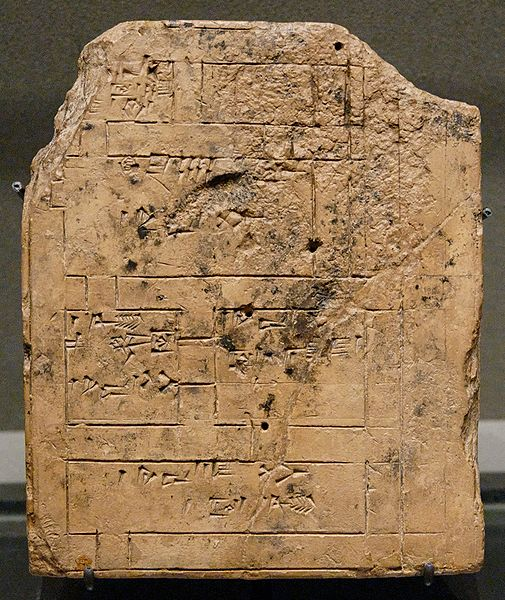
\includegraphics[width=\linewidth]{gudea-plans}
  \caption{Clay plans of a six-room building, a sanctuary or a private house. From Telloh, ancient Girsu circa 2125, from \url{http://en.wikipedia.org/wiki/Gudea_cylinders}}
  \label{fig:marginfig1}
\end{marginfigure}
If you ever lost a document you will agree that there is always a need to keep control of important documents. The document control system has been designed to aid in the  filing of documents and provide an easy way of retrieving this information.
Some documents we keep because is required by law to keep them. Others we need them in order to control the flow of money in a Company. To summarize the system described in this chapter will help you file your documents better and enable you to retrieve these documents easier.

\section*{What is document control?}

Document control means that the right persons have the current version of the documents they need, while unauthorized persons are prevented access to them.

We all handle many documents every day. These documents include forms that we fill out, instructions that we follow, invoices that we enter into the computer system, holiday schedules that we check for the next day off, rate sheet that we use to bill out customers, and many more.

An error on any of these documents could lead to problems. Using an outdated version could lead to problems. Not knowing if we have the latest version or not could lead to problems. And so on.

The Document control system affects our entire company, and all business related documents must be controlled. Only documents that don’t have an impact on our products, services or company don’t need to be controlled – all others need to be controlled. This means, basically, that any business related documents must be controlled. 

\section*{Whose responsibility?}

\begin{marginfigure}
  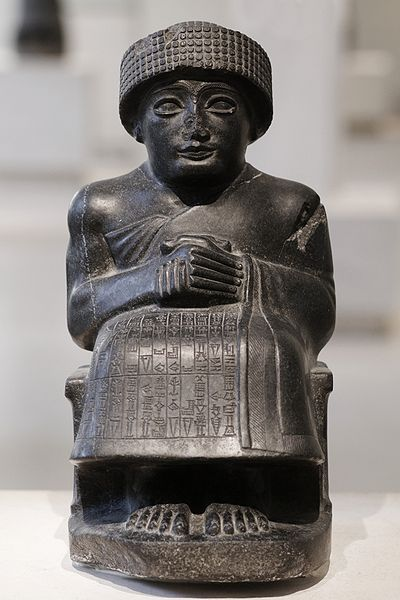
\includegraphics[width=\linewidth]{gudea}
  \caption{Diorite statue od the earliest known document Controller. Mesopotamia circa 2150 BC.}
  \label{fig:marginfig1}
\end{marginfigure}

Document control is the responsibility of all employees. It is important that all employees understand the purpose of document control and the tools (requirements) that help us control our documents.

Please be aware that if you copy a document or print one out and then distribute it, you are responsible for controlling the distribution! The original author won't know that you distributed more of his documents, so the original author can't control that distribution. That is why on critical job sites all copies, faxing and distribution is via our DCC (Document Control Center)






\section*{Project Filing}

%\begin{marginfigure}
%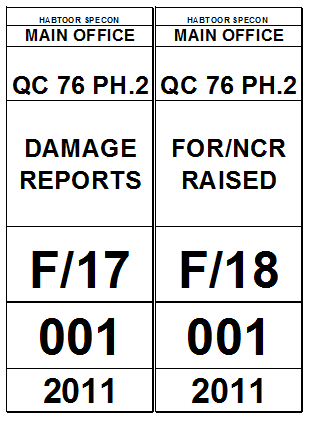
\includegraphics[width=\linewidth]{labels}
%\caption{Filing labels}
%\end{marginfigure}

\begin{marginfigure}
  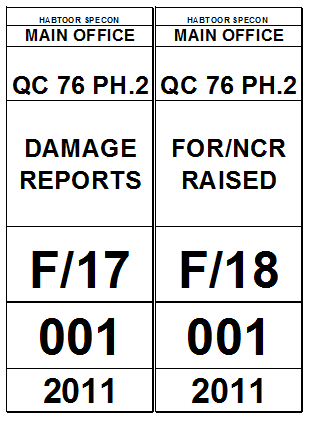
\includegraphics[width=\linewidth]{labels}
  \caption{Calorifier plant-room in Merweb.}
  \label{fig:marginfig1}
\end{marginfigure}

Project filing, follows closely to the system set up at Head Office. You can think of Document Control a bit like the post office where communication is always between one office to another. In many respects filing on sites is more difficult and challenging due to its temporary nature and the changing number of employees as the Project moves through the different phases.

Files are labeled with letters and numbers:

\begin{center}
\fbox{
       \begin{minipage}{6.0cm}
        FILE REF. NO. A/1

        Outgoing Correspondence.
       \end{minipage}
}
\end{center}
        
When files overflow we number them consequentially as follows:

\begin{center}
\fbox{
       \begin{minipage}{6.0cm}
        FILE REF. NO. A/1-001

        Outgoing Correspondence.

        FILE REF. NO. A/1-002

        Outgoing Correspondence.
 \end{minipage}
}
\end{center}

The file references are initially chosen to represent a comprehensive Master File list. An extract from such a Master List is in Table\ref{masterlist}.


\begin{fullwidth}
\begin{table}[htb]
\vspace{0.5cm}

\small
\hskip-10pt\begin{tabular}{|l|l|l|l||l|l||l|l||l|l|l|}
\hline
File &Category        &Control              & Person       &Copy 1  &Person        &Copy 2        &Person      &Copy 3 &Person\\
     &                &Copy location        & resp. &        &resp.   &resp.   &resp. &      &resp.\\
\hline
A/1    & Corresp (in).       & H.O. Sec.           & H.O. Secr. & Site & PM           &              &            &      & \\
A/2    & Corresp.(out)       & H.O. Sec.           & H.O. Secr. & Site & PM           &              &            &      & \\
A/3    & memos (in)          & H.O. Sec.           & H.O. Secr. & Site & PM           &              &            &      & \\
A/4    & memos (out)         & H.O. Sec.           & H.O. Secr. & Site & PM           &              &            &      & \\
\hline
\end{tabular} 	
\caption{Extract from filing list}
\label{masterlist}
\end{table}
\end{fullwidth}

What is important to notice in the Table above, that in many cases the filing system allows for up to three copies to be kept, but there is always a two tier system where there is a \textit{control copy}, normally kept at head office and one or two copies kept at other locations. If the site is far from head office or for cases where there is no need to keep copies at Head Office the Document Control Department always keeps the master copy.

It is also important to note that documents have \textit{owners}. In the extract shown in Table\ref{masterlist}. The owner is the responsible person to make sure that the documents have been filed properly. In most cases this person in the Project Document Controller, but for example for orders the Materials Control Manager is the ultimate responsible person to ensure that MCD documents are filed properly.

\subsection*{Document Order}

In general document are filed by \textit{date order}. Numbered documents such as submittals, Quality Assurance Documents and the like bear that bear \textit{reference numbers} are filed \textit{sequentially}. Accounting documents
such as creditors invoices are filed by \textit{date} in the master file and a second copy by \textit{Creditors name}. By choosing
carefully the method of filing and normally by having two different methods enables retrieval of the document easier. In general if the system
is computerized retrieval becomes easier.  

\section*{Setting up the system}

The filing system should be set at the begining of a new Project. Although this sounds simple and intuitive most Projects start without adequate
space, building shelving as we go and continuously buying files. On a well designed system \textit{all} file categories are set up when the Project starts, they are labelled uniformly. As a rule of thumb the minimum space is that of a 20 foot container - and this assuming that files with multiple volumes are archived at certain points. If you do not give it attention at the beginning of the Project you will literally
drawn in paper work nobody will be able to find anything and  everyone will build their own system as they will not have any \textit{faith} in yours!

The equation below, can be used to estimate the number of files that will be required for a project:



$$ N = \frac{p^{0.8}(t + d)}{d} $$

where,

N = number of files

p = mean personnel on project

t = duration of project (months)

d = number of departments




\section*{When to file}

Generally if people responsible for filing do not clear their intrays daily it leads to problems with retrieval. What happens as they have a continuous backlog the bottom of the tray never gets cleared and after a week or two documents cannot be found (so we get another copy from whoever sent it to us) which leads to another problem that eventually when we find the document we now have two identical copies in the file and 
stamped with two different incoming date stamps.

\section*{Getting the right equipment}

During the two critical \textit{crunch periods} of the Project, which are normally the start and end of the Project you will find that
documents and document copying and processing is at its peak. During this time of the project unless the Site and its partner Companies have a decent photocopier the flow of documents will slow down tremendously. It is not unknown for documents to take 11 days to be delivered from the Consultant's desk (via their own document control) to that of the Main contractors's and then to us. For comparison in 1890 a letter would travel at the cost of 1 penny with the Imperial Penny Post from London to Cape Town by steam ship in less than 20 days and taht was door to door delivery. In general a decent photocopier should be purchased based on expected volumes of copying which should never be less than 20000 copies per month (to keep up with peaks). This should be able to interface with a computer and the network and if you are going to charge subcontractors  departments or Clients it should have a keypad for logging usage. When the latter is not used, it is also not unknown for people to introduce 
manual systems of approval and logging of copies usage introducing another cost to the Company and further contributing to bureacratic bloat, inefficiency and delays. 

\section*{Key performance indicators}

Document Control should be able to produce all necessary log forms weekly by close of business every Thursday or at a date agreed with the Project Director. Normally these are:

\begin{table}
\begin{tabular}{l}
\toprule
Material Submittal logs\\
RFI logs\\
WIR logs\\
\bottomrule
\end{tabular}
\caption{Weekly logs produced by Document Control}
\end{table}


Document Control should be able to retrieve a document within a maximum of 30 minutes and deliver a copy (right? you don't want the original copies to leave Document Control - so you do need a good and fast photocopier). The best performance indicator is for the Document Control Department is to keep it \textit{customers} happy. 

\section*{Dating documents}

Require us to show on every document when it was created or last updated. Many of us thought about using the automatic date field for this but….
Should we use the automatic date field on documents?

Generally not, if you enter the automatic date field into a document, the field will automatically be updated to always show the current date, no matter when you actually created or updated the document.



Another example:

Another example is entering the automatic date field in the footer of a document that you frequently change and then print. You may have used the automatic date field as an easy way to see on your printouts when they were printed; the idea here was that the document with the latest date is the most current printout. However, you may make one printout today and another tomorrow without having made any changes to the document. Though both printouts are identical, they now show different dates. This will inevitably lead to confusion. 

Document control requires us to show on any document when it was created or last updated. The automatic date field is not suitable for this. Therefore, as a general rule, don’t use the automatic date field to identify version status.


\section*{Forms}

Yes, a form must be controlled as long as the form has an impact on our services or our company.

Blank forms are similar to instructions as they guide the user to provide certain information. If the form is outdated or incomplete, the user will not be prompted to supply all the necessary information. It is, therefore, important to control blank forms like any other document.

Once a form is filled out, however, it has become a record. At this point, we need to be concerned with filing, storage, archiving, and eventually destruction.
All forms and documents are specified in the Company ISO Manual.

\section*{Policies and procedures}

While most procedure affect only managers, all employee must be familiar with the \textit{Quality Policy} and with the \textit{Document Control Procedure}.

\section*{Document Control Organization}

The Document control department is actually a Main Department and sattelites. Sattelite sections will exist in other Departments. In general it should be organized as follows:

\begin{verbatim}
- Document Control (Central Department)
-- Administration /HR (visa related, personnel passports, drivers, petrol control)
-- Correspondence (secretary)
-- QA/QC
-- QS
-- Procurement
-- Design (very limited)
-- CAD Office
-- Accounts
-- Stores (own copies of delivery notes, returns issues etc).
-- Safety department
\end{verbatim}

The particular contributions of these departments are laid out in their respective Business process sections. The Document Control department is normally staffed with 3-4 people. The Document Controller, one or two assistants and a person dedicated to photo-copying. 


\section*{Computerized Systems}

Computerized systems do not eliminate the need for paper filing but can reduce it. They can also assist in retrieval and distribution. Unless
your manual system is working well, computerization is next to impossible.


\section*{Archiving and disposal of documents}
\begin{marginfigure}
  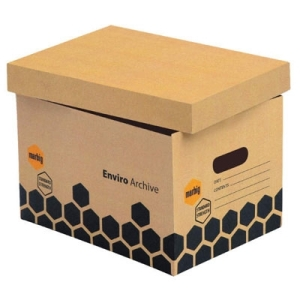
\includegraphics[width=\linewidth]{archivebox}
  \caption{Environmental friendly box}
  \label{fig:marginfig1}
\end{marginfigure}
At the end of the Project most of the items will require to be disposed or archived. Having now contributed considerably to the destruction of the environment by using all this paper and possibly finished a monstrosity on a pristine location, this can be done by buying environmentally friendly boxes made for the purpose. Documents to be disposed should be shredded if possible. If the system has been followed and monitored, this should be a simple operation as all the filing will already be in boxes and what it means is that only the last files will be boxed. Label the boxes accordingly and state the date that the contents can be disposed off.

\section*{Summary}

This short document described some of the issues relating to the control of Company documents. As a last word do some kaizen.\sidenote{\href{Kaizen}{http://en.wikipedia.org/wiki/Kaizen}.}






























\chapter{Materials Control Department}

\begin{quotation}
 If you're buying a product then you need to spend money to hire sophisticated buyers, because if your buyers are dumber than the sales-people you're buying from they're going to be fleeced.
\end{quotation}

The Materials Control Department on a Project is the responsible department that ensures that materials are purchased at the \textit{least possible price, they
meet the Project quality standards  and that they are delivered on time}. 

\section*{Materials Planning}
This is the most difficult phase of teh procurement cycle and if not planned
properly the MCD department will be in \textit{panic mode} until the end of the
Project. At the beginning of the Project a Materials Control Sheet is created
listing all the material requirements of the Project by categories. Categories
are normally split in such a way that a category is materials purchased from a single
vendor.

At the beginning of the Project at the discretion of the Area Manager and the Project
Director, the Engineering Office as well as all the Engineers and perhaps the
CAD Office will contribute to material take-offs. The Engineering Office
will also handle enquiries and discussions with Suppliers for items where
a strong technical input is required. Here is a short list, however what is important
is to generate such lists comprehensively at the beginning of the Project. It is the 
responsibility of the MCD Manager to monitor progress and to produce weekly reports.

\begin{fullwidth}
\begin{table}[htbp]
\vspace{0.5cm}
\begin{tabular}{clllp{3cm}}
\toprule
Item  &Responsibility &Technical submittal &Remarks\\
\midrule
\inc &AHUs  & Engineering Office & Engineering Office & take-offs by Section Engineers\\
\inc &fcus  & Engineering Office & Engineering Office & take-offs by Section Engineers\\
\inc &Chillers  & Engineering Office & Engineering Office & take-offs by Section Engineers\\
\inc &Pumps & Engineering Office & Engineering Office & take-offs by Section Engineers\\
\inc &Package Units  & Engineering Office & Engineering Office & take-offs by Section Engineers\\
\inc &Fans  & Engineering Office & Engineering Office & take-offs by Section Engineers\\
\inc &ECUs  & Engineering Office & Engineering Office & take-offs by Section Engineers\\
\bottomrule
\end{tabular}
\caption{Mechanical long lead items}
\label{longleaditems}
\end{table}
\end{fullwidth}

It is noteworthy, that all the equipment listed above need to have static calculations in order for orders to be finalized. This is not always possible to be carried out at the beginning of the Project
and is best to agree with the Supplier cut-off dates for the supply of this information. In general
if you adhere to the following process things are easier\sidenote{With software these calculations are not difficult to produce, if the Tender drawings are reasonably well co-ordinated.}:

\begin{enumerate}
\item Send out enquiries early based on Tender documents.
\item Narrow down the price with one Supplier.
\item Work with the Supplier to obtain selections and submittals.
\end{enumerate}

Although it is important not to lose time and long-lead items need to be ordered as early as possible
it is also very important to act quickly and get approvals and orders out for first fix materials. 

\begin{fullwidth}
\begin{table}[htbp]
\vspace{0.5cm}
\begin{tabular}{clllp{3cm}}
\toprule
Item  &Responsibility &Technical submittal &Remarks\\
\midrule
\inc &anchors  & Engineering Office & Engineering Office & take-offs by Section Engineers\\
\inc &threaded rods  & Engineering Office & Engineering Office & take-offs by Section Engineers\\
\inc &supports  & Engineering Office & Engineering Office & take-offs by Section Engineers\\
\inc &unistrut  & Engineering Office & Engineering Office & take-offs by Section Engineers\\
\inc &insulation inserts  & Engineering Office & Engineering Office & take-offs by Section Engineers\\
\inc &conduit systems  & Engineering Office & Engineering Office & take-offs by Section Engineers\\
\bottomrule
\end{tabular}
\caption{Mechanical first fix items}
\label{firstfixitems}
\end{table}
\end{fullwidth}

Table \ref{firstfixitems} if handled properly and quickly they enable operations to start on Site.
There is no benefit in focusing first on pipes and fittings, if the above will not have an approval
and there is no stock on site to start the works. These materials should be closed in the first 3-4 weeks of the Project. 


\begin{fullwidth}
\begin{table}[htbp]
\vspace{0.8cm}
\begin{tabular}{clllp{3cm}}
\toprule
Item  &Responsibility &Technical submittal &Remarks\\
\midrule
\inc &drainage pipes  & Engineering Office & Engineering Office & take-offs by Section Engineers\\
\inc &chilled water pipes  & Engineering Office & Engineering Office & take-offs by Section Engineers\\
\inc &fire protection pipes  & Engineering Office & Engineering Office & take-offs by Section Engineers\\
\inc &H\&C water piping & MCD & MCD/EO & BOQ Section Engineers\\
\inc &Cable trays & MCD & MCD/EO & BOQ Section Engineers\\
\inc &Cable ladders & MCD & MCD/EO & BOQ Section Engineers\\
\inc &ductwork & MCD & MCD/EO & BOQ Section Engineers\\
\bottomrule
\end{tabular}
\caption{Mechanical first fix items (second tier)}
\label{firstfixitems}
\end{table}
\end{fullwidth}


\section*{Second and Third Fix Materials}
Depending on the Project and its requirements second and third fix materials are tackled next. 
The list below is not comprehensive, but should mre or less be prioritized as shown. Keep in
mind what you need to complete the installation and what is affecting follow-up trades such as
the Main Contractor cosing walls or ceilings.

\begin{fullwidth}
\begin{table}[htbp]
\vspace{0.8cm}
\begin{tabular}{clllp{3cm}}
\toprule
Item  &Responsibility &Technical submittal &Remarks\\
\midrule
\inc &drainage specialties  & Engineering Office & Engineering Office & take-offs by Section Engineers\\
\inc &interceptors& Engineering Office & Engineering Office & take-offs by Section Engineers\\
\inc &manhole covers& Engineering Office & Engineering Office & take-offs by Section Engineers\\
\inc &paddle-flanges& Engineering Office & Engineering Office & take-offs by Section Engineers\\
\inc &special sleeves& Engineering Office & Engineering Office & take-offs by Section Engineers\\
\bottomrule
\end{tabular}
\caption{Drainage materials}
\label{firstfixitems}
\end{table}
\end{fullwidth}

As for the drainage materials, focus is being maintained as to what is needed next. For HVAC is making sure that what is required in terms of ductwork and piping.

\begin{fullwidth}
\begin{table}[htbp]
\vspace{0.8cm}
\begin{tabular}{clllp{3cm}}
\toprule
Item  &Responsibility &Technical submittal &Remarks\\
\midrule
~ &\textbf{Ducted systems}&  &  & \\
\inc &Fire Dampers& Engineering Office & Engineering Office & take-offs by Section Engineers\\
\inc &Volume Dampers & Engineering Office & Engineering Office & take-offs by Section Engineers\\
\inc &Motorized Dampers & Engineering Office & Engineering Office & take-offs by Section Engineers\\
\inc &Access Doors & Engineering Office & Engineering Office & take-offs by Section Engineers\\
\inc &Sound attenuators & Engineering Office & Engineering Office & take-offs by Section Engineers\\
\inc &Flexible ducts & Engineering Office & Engineering Office & take-offs by Section Engineers\\
\inc &Flexible connectors & Engineering Office & Engineering Office & take-offs by Section Engineers\\
\inc &Grilles \& Diffusers & Engineering Office & Engineering Office & take-offs by Section Engineers\\
\inc &Louvres  & Engineering Office & Engineering Office & take-offs by Section Engineers\\
\inc &Sand-trap louvres  & Engineering Office & Engineering Office & take-offs by Section Engineers\\
\midrule
~ &\textbf{Piping Systems} &  &  &  \\
\inc &Valves  &EO   &EO  &EO/CAD \\
\inc &Flanges &  &  &\\
\inc &Gaskets &  &  &\\
\inc &Bolts   &  &  &\\
\inc &Insulation & & &\\
\inc &Insulation accessories & & &\\
\inc &Chemical treatment & & &\\
\inc &Pressurization units & & &\\
\inc &Expansion vessels & & &\\
\inc &De-aerators & & &\\
\midrule
~ &\textbf{BMS \& Controls} &  &  &  \\
\inc &BMS General & & &\\
\inc &BMS Graphics & & &\\
\inc &BMS Cables   & & &\\
\bottomrule
\end{tabular}
\caption{HVAC material lists}
\label{firstfixitems}
\end{table}
\end{fullwidth}

If everything has been co-ordinated properly, orders are placed on agreed staged deliveries or to
draw as per Site requirements. When you place orders full at the beginning of the Project you
save considerable trouble, you manage less documents, less submittals etc. In general on most
jobs, there will be about 150-160 categories of materials. On a target to close between 2-3 categories daily in the first 90 days of the project you will need 3-4 people to process, plus of course the full site Team should be contributing to this. It is the responsibility of the Project Manager to arrange a meeting where \textit{names} are put next to each material to ensure action and responsibilities are clear cut and the materials are processed as fast as possible.


\section*{Stock control for consumables}

Two bin systems are common on assembly and moving manufacturing lines where components are added to the product or item being built. The two bin system is just like its name suggests, it is composed of two bins which are full of components or materials to start. As production commences one bin is drawn down of materials and the other bin, which is still full, acts as the buffer or safety stock.

When the first bin is completely depleted the worker or assembly line worker switches to the other bin, similar to a FIFO system. The switch of bins can be interpreted as a kanban signal for the supply process of that particular component to manufacture or supply the component just in time before the second bin runs out of material. The kanban signal can also be generated half way throughout the first bin, depending on lead times for the component to be supplied. 

This system in a way is similar to the EOQ inventory model with safety stock. It is a very common system used in vehicle manufacturing plants. The size or number of components in each bin is usually determined using the EOQ inventory model or a time period model. 
\chapter{Planning}

Planning the works needs no introduction, but the reality is that most Engineers
do very little planning of their works whereas many others understand that planning
is something done at the beginning of a Project using Primavera and the rest is just following the direction of the Project as it goes.

There are many elements of planning and before we get onto that we will analyse them in details. In many respects planning is like waterpainting, you start sketiching to see what you want to achieve and then you detail it as you go along.

\begin{fullwidth}
\begin{figure*}
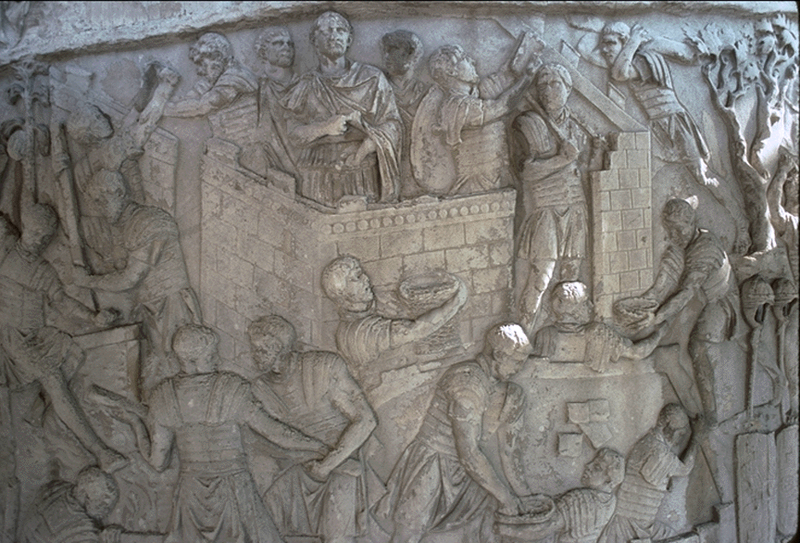
\includegraphics[width=1.1\textwidth]{./graphics/trajan-column}
\caption{Roman soldiers building a fortress, Trajan's Column 113 AD}
\end{figure*}
\end{fullwidth}

Planning is both the organizational process of creating and maintaining a \textit{plan}; and the psychological process of thinking about the activities required to create a desired goal.

\section*{Determining the right sequence of works}

Before any plan is drawn some understanding of the sequence of works
is necessary. Activities can be divided into sequential or parallel. A
sequential activity is one that you cannot start unless a previous activity
has been completed. If the activity of having procured the materials is not
completed, then the works cannot be started. 

\section*{How do I start}

The first thing you need to do before you start is to identify the \textit{goal}.
In many cases this is not that difficult, but you will find out that the goal as
stated is too theoretical and you need to cut it down to smaller objectives.

We will discuss techniques by means of focusing on examples which are smaller.
In my opinion this is where most people fail to plan properly and let events
overtake them. We will assume that shop drawings are available and that materials
are also available and that we will use a Team of Duct erectors.

\subsection*{Measure your target}

Unless you measure something, you cannot control it. If you know that you have to install 600 m$^2$ of ductwork, you may be in a better position to estimate the time
it takes to install it (provided that you have some background information). 


\begin{marginfigure}
The Tower can be represented by a series of squares, which denote an activity. Green is done and white is not done. There is no need to use intermediate colors. they just detract from the visual information.
\vspace{1cm}
%% Color definitions




\floor{Level 47}{0}{0}{0}{0}{2}
\floor{Level 46}{0}{0}{0}{2}{2}
\floor{Level 45}{0}{0}{1}{1}{1}
\floor{Level 44}{0}{0}{1}{1}{1}
\floor{Level 43}{1}{1}{1}{1}{1}
\floor{Level 42}{1}{1}{1}{1}{1}
\floor{Level 41}{0}{1}{1}{0}{1}
\floor{Level 40}{0}{1}{1}{1}{1}
\floor{Level 39}{0}{1}{1}{1}{1}
\floor{Level 38}{0}{1}{1}{1}{1}
\floor{Level 37}{0}{0}{1}{1}{1}
\floor{Level 36}{0}{0}{0}{1}{1}
\floor{Level 35}{0}{0}{0}{1}{1}
\floor{Level 34}{0}{0}{0}{1}{1}
\floor{Level 33}{0}{0}{0}{1}{1}
\floor{Level 32}{0}{0}{0}{1}{1}
\floor{Level 31}{0}{0}{0}{1}{1}
\floor{Level 30}{0}{0}{0}{1}{1}
\floor{Level 29}{1}{1}{1}{1}{1}
\floor{Level 28}{1}{1}{1}{1}{1}
\floor{Level 27}{0}{1}{1}{1}{1}
\floor{Level 26}{0}{1}{1}{1}{1}
\floor{Level 25}{0}{0}{1}{1}{1}
\floor{Level 24}{0}{0}{1}{1}{1}
\floor{Level 23}{0}{0}{1}{1}{1}
\floor{Level 22}{0}{0}{1}{1}{1}
\floor{Level 21}{0}{0}{1}{1}{1}
\floor{Level 20}{0}{0}{1}{1}{1}
\floor{Level 19}{0}{0}{1}{1}{1}
\floor{Level 18}{0}{0}{1}{1}{1}
\floor{Level 17}{0}{0}{1}{1}{1}
\floor{Level 16}{0}{0}{1}{1}{1}
\floor{Level 15}{0}{1}{1}{1}{1}
\floor{Level 14}{0}{1}{1}{1}{1}
\floor{Level 12}{0}{1}{1}{1}{1}
\floor{Level 11}{0}{1}{1}{1}{1}
\floor{Level 10}{1}{1}{1}{1}{1}
\floor{Level 09}{1}{1}{1}{1}{1}
\floor{Level 08}{1}{1}{1}{1}{1}




%
%\begin{tikzpicture}[scale=0.8]
%\draw node [anchor=south east]{Level 08};
%\draw (0,0) rectangle (0.5,0.5);
%\draw  [fill=green] (0.6,0.0) rectangle (1.1,0.5) ;
%\draw [fill=green] (0.6+0.6,0.0) rectangle (1.7,0.5) ;
%\draw[fill=green]  (3*0.6,0.0) rectangle (2.3,0.5) ;
%\draw[fill=green]  (4*0.6,0.0) rectangle (2.9,0.5) ;
%\node at (4,0.1) {Apart. 90\%};
%\end{tikzpicture}
%\def\addlegend#1#2{% color label
%  \begin{tikzpicture}[scale=0.8]
%   \draw[fill=#1] (0,0) rectangle (0.5,0.5);
%   \draw node [anchor=south east]{#2};
%   \end{tikzpicture}\vspace{2pt}}
%\addlegend{green}{lights}
\caption{Rotana Tower Progress, each square represents one separate activity}
\end{marginfigure}


When you first start with the plan, a visual representation of the
areas and work you will be working on can be invaluable. For example
a layout of the area with some coloring can help you identify better
to visualize the problem. At this point if the area is available, you
should visit the area and get a feeling of the problems that you may 
encounter. Once you have a good idea of what you want to achieve, you need to translate
it into something more definable. For ductwork we would normally divide
the work as shown in \ref{ductplan}. For most MEP activities is almost
a rule that unless you put a Team to start by installing supports, it is 
almost certain that manhours will be lost later on. By starting supports early
you ensure that the charge-hand who is marking the support locations is
scouting the area and ensuring that there are no impediments. In very rare
occassions that this is not necessary, such as ductwork in plantrooms.

\pagebreak
\gdef\ascale{0.65}
\begin{minipage}{4cm}
\small
\floor{Level 47}{0}{0}{0}{0}{2}
\floor{Level 46}{0}{0}{0}{2}{2}
\floor{Level 45}{0}{0}{1}{1}{1}
\floor{Level 44}{0}{0}{1}{1}{1}
\floor{Level 43}{1}{1}{1}{1}{1}
\floor{Level 42}{1}{1}{1}{1}{1}
\floor{Level 41}{0}{1}{1}{0}{1}
\floor{Level 40}{0}{1}{1}{1}{1}
\floor{Level 39}{0}{1}{1}{1}{1}
\floor{Level 38}{0}{1}{1}{1}{1}
\floor{Level 37}{0}{0}{1}{1}{1}
\floor{Level 36}{0}{0}{0}{1}{1}
\floor{Level 35}{0}{0}{0}{1}{1}
\floor{Level 34}{0}{0}{0}{1}{1}
\floor{Level 33}{0}{0}{0}{1}{1}
\floor{Level 32}{0}{0}{0}{1}{1}
\floor{Level 31}{0}{0}{0}{1}{1}
\floor{Level 30}{0}{0}{0}{1}{1}
\floor{Level 29}{1}{1}{1}{1}{1}
\floor{Level 28}{1}{1}{1}{1}{1}
\floor{Level 27}{0}{1}{1}{1}{1}
\floor{Level 26}{0}{1}{1}{1}{1}
\floor{Level 25}{0}{0}{1}{1}{1}
\floor{Level 24}{0}{0}{1}{1}{1}
\floor{Level 23}{0}{0}{1}{1}{1}
\floor{Level 22}{0}{0}{1}{1}{1}
\floor{Level 21}{0}{0}{1}{1}{1}
\floor{Level 20}{0}{0}{1}{1}{1}
\floor{Level 19}{0}{0}{1}{1}{1}
\floor{Level 18}{0}{0}{1}{1}{1}
\floor{Level 17}{0}{0}{1}{1}{1}
\floor{Level 16}{0}{0}{1}{1}{1}
\floor{Level 15}{0}{1}{1}{1}{1}
\floor{Level 14}{0}{1}{1}{1}{1}
\floor{Level 12}{0}{1}{1}{1}{1}
\floor{Level 11}{0}{1}{1}{1}{1}
\floor{Level 10}{1}{1}{1}{1}{1}
\floor{Level 09}{1}{1}{1}{1}{1}
\floor{Level 08}{1}{1}{1}{1}{1}
\end{minipage}
\hspace{1em}
\begin{minipage}{4cm}
\small
\floor{Level 47}{0}{0}{0}{0}{2}
\floor{Level 46}{0}{0}{0}{2}{2}
\floor{Level 45}{0}{0}{1}{1}{1}
\floor{Level 44}{0}{0}{1}{1}{1}
\floor{Level 43}{1}{1}{1}{1}{1}
\floor{Level 42}{1}{1}{1}{1}{1}
\floor{Level 41}{0}{1}{1}{0}{1}
\floor{Level 40}{0}{1}{1}{1}{1}
\floor{Level 39}{0}{1}{1}{1}{1}
\floor{Level 38}{0}{1}{1}{1}{1}
\floor{Level 37}{0}{0}{1}{1}{1}
\floor{Level 36}{0}{0}{0}{1}{1}
\floor{Level 35}{0}{0}{0}{1}{1}
\floor{Level 34}{0}{0}{0}{1}{1}
\floor{Level 33}{0}{0}{0}{1}{1}
\floor{Level 32}{0}{0}{0}{1}{1}
\floor{Level 31}{0}{0}{0}{1}{1}
\floor{Level 30}{0}{0}{0}{1}{1}
\floor{Level 29}{1}{1}{1}{1}{1}
\floor{Level 28}{1}{1}{1}{1}{1}
\floor{Level 27}{0}{1}{1}{1}{1}
\floor{Level 26}{0}{1}{1}{1}{1}
\floor{Level 25}{0}{0}{1}{1}{1}
\floor{Level 24}{0}{0}{1}{1}{1}
\floor{Level 23}{0}{0}{1}{1}{1}
\floor{Level 22}{0}{0}{1}{1}{1}
\floor{Level 21}{0}{0}{1}{1}{1}
\floor{Level 20}{0}{0}{1}{1}{1}
\floor{Level 19}{0}{0}{1}{1}{1}
\floor{Level 18}{0}{0}{1}{1}{1}
\floor{Level 17}{0}{0}{1}{1}{1}
\floor{Level 16}{0}{0}{1}{1}{1}
\floor{Level 15}{0}{1}{1}{1}{1}
\floor{Level 14}{0}{1}{1}{1}{1}
\floor{Level 12}{0}{1}{1}{1}{1}
\floor{Level 11}{0}{1}{1}{1}{1}
\floor{Level 10}{1}{1}{1}{1}{1}
\floor{Level 09}{1}{1}{1}{1}{1}
\floor{Level 08}{1}{1}{1}{1}{1}
\end{minipage}
\hspace{0.8cm}
\begin{minipage}{4cm}
\small
\floor{Level 47}{0}{0}{0}{0}{2}
\floor{Level 46}{0}{0}{0}{2}{2}
\floor{Level 45}{0}{0}{1}{1}{1}
\floor{Level 44}{0}{0}{1}{1}{1}
\floor{Level 43}{1}{1}{1}{1}{1}
\floor{Level 42}{1}{1}{1}{1}{1}
\floor{Level 41}{0}{1}{1}{0}{1}
\floor{Level 40}{0}{1}{1}{1}{1}
\floor{Level 39}{0}{1}{1}{1}{1}
\floor{Level 38}{0}{1}{1}{1}{1}
\floor{Level 37}{0}{0}{1}{1}{1}
\floor{Level 36}{0}{0}{0}{1}{1}
\floor{Level 35}{0}{0}{0}{1}{1}
\floor{Level 34}{0}{0}{0}{1}{1}
\floor{Level 33}{0}{0}{0}{1}{1}
\floor{Level 32}{0}{0}{0}{1}{1}
\floor{Level 31}{0}{0}{0}{1}{1}
\floor{Level 30}{0}{0}{0}{1}{1}
\floor{Level 29}{1}{1}{1}{1}{1}
\floor{Level 28}{1}{1}{1}{1}{1}
\floor{Level 27}{0}{1}{1}{1}{1}
\floor{Level 26}{0}{1}{1}{1}{1}
\floor{Level 25}{0}{0}{1}{1}{1}
\floor{Level 24}{0}{0}{1}{1}{1}
\floor{Level 23}{0}{0}{1}{1}{1}
\floor{Level 22}{0}{0}{1}{1}{1}
\floor{Level 21}{0}{0}{1}{1}{1}
\floor{Level 20}{0}{0}{1}{1}{1}
\floor{Level 19}{0}{0}{1}{1}{1}
\floor{Level 18}{0}{0}{1}{1}{1}
\floor{Level 17}{0}{0}{1}{1}{1}
\floor{Level 16}{0}{0}{1}{1}{1}
\floor{Level 15}{0}{1}{1}{1}{1}
\floor{Level 14}{0}{1}{1}{1}{1}
\floor{Level 12}{0}{1}{1}{1}{1}
\floor{Level 11}{0}{1}{1}{1}{1}
\floor{Level 10}{1}{1}{1}{1}{1}
\floor{Level 09}{1}{1}{1}{1}{1}
\floor{Level 08}{1}{1}{1}{1}{1}
\end{minipage}

\pagebreak
\def\don#1{\cellcolor[gray]{0.9}#1}  %{0.9}
\setcounter{inc}{0} % reset counter
\begin{table}[htbp]
\vspace{0.8cm}
\small
\begin{tabular}{|l|p{3.9cm}|l|l|l|l|l|l|l|l|}
\hline
item  &Description  &Qty   &Week 1 &Week 2 &Week 3 &Week 4 &Week 5 &Week 6 &Total\\
\hline
\inc     &supports &400 &\don{100} &\don{100} &\don{100} &\don{100} & & &\\
\inc     &ductwork (insulated) &1200 &\don{200} &\don{200} &\don{200} &\don{200} &\don{200} &\don{200} &\\
\inc     &ductwork (uninsulated) & 600 & & & & & & &\\
\inc     &vol. dampers & & & & & & & &\\
\inc     &fire dampers & & & & & & & &\\
\inc     &flexibles & & & & & & & &\\
\inc     &WIR   & & & & & & & &\\      
\hline
\end{tabular}
\caption{Example of 6 week look-ahead program for installation of ductwork.}
\label{ductplan}
\end{table}

\setcounter{inc}{0} % reset counter
\begin{table}[htbp]
\vspace{0.8cm}
\small
\begin{tabular}{|l|p{3.9cm}|l|l|l|l|l|l|l|l|}
\hline
item  &Description  &qty   &unit & manhours &$f_1$ &$f_2$ &$f_3$ &$f_4$ &Total\\
\hline
\inc     &supports &400 &each & & & & & &\\
\inc     &ductwork (insulated) &1200 &m$^2$ & & & & & &\\
\inc     &ductwork (uninsulated) & 600 &m$^2$ & & & & & &\\
\inc     &vol. dampers &80 &each & & & & & &\\
\inc     &fire dampers &20 &each & & & & & &\\
\inc     &flexibles &60 &each & & & & & &\\
\inc     &WIR   &5 &each & & & & & &\\      
\hline
\end{tabular}
\caption{Example of 6 week look-ahead program for installation of ductwork.}
\label{ductplan}
\end{table}


The factors $f_1, f_2, f_3, f_4$ are a series of factors that ca be used to
adjust your estimate based on your observations of the rate of the works and
the actual conditions that the work is taking place.

$f_1$ = congestion factor.

$f_2$ = weather factor.

$f_3$ = team expertise.

$f_4$ = overtime work.

Of importance is to note that your budget for overtime works will increase
the total manhours that are required to complete the works, as overtime work
in general reduces efficiency of personnel.

The above costs are estimated to be on the low side. Published tables are frequently used to quantify loss of productivity for scheduled overtime [18,19,20,21], overmanning [22,23,24], congestion of trades [23], remobilization [22], and weather [25,26,27].

In this Project the Contractor accelerated completion activities in many areas in order to follow the program. Loss of productivity occurred as a result of overtime due to a number of reasons: fatigue; demotivation; absenteeism; reduction of workpace and congestion, see Figure \ref{fig:congestion}; The factors most commonly cited in the literature are those prepared by the Construction Users' Anti-Inflation Roundatable\sidenote{Construction Users' Anti-Inflation Roundtable, `'Overtime in Construction'', AACE Bulletin, Vol. 15, No. 5, October 1973.}, shown in Figure \ref{fig:overtime}. These impacts have not be taken into account in the above calculations, as the Contractor was aware that overtime, however, inefficient had to be introduced to complete the works by the agreed date. However, not all these costs belong to the Contractor as the Contractor attempted to coomplete Engineer's Instructions and other changes as quick as possible.


\begin{figure}[htbp]
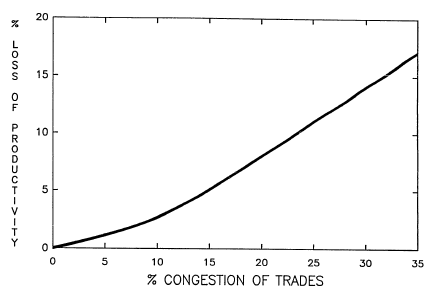
\includegraphics[width=0.9\textwidth]{./graphics/AHU/congestion}
\caption{Impact of overtime on productivity}
\label{fig:overtime}
\end{figure}


\begin{figure}[htbp]
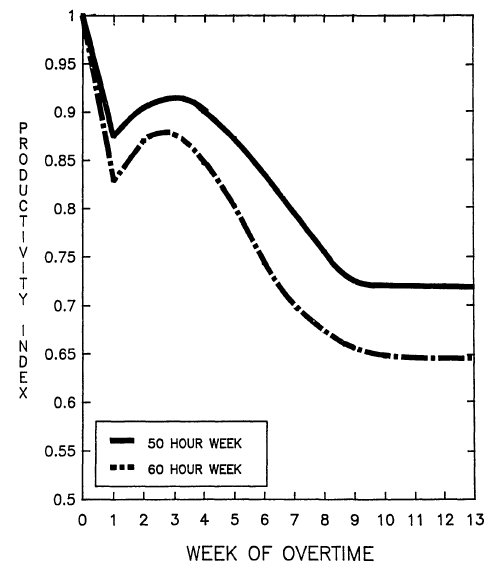
\includegraphics[width=0.8\textwidth]{./graphics/AHU/overtime}
\caption{Impact of overtime on productivity}
\label{fig:congestion}
\end{figure}


The major cause of schedule disruptions and delays all related to lack of information and change orders. Essentially, all causes beyond the Contractor's control

\subsection{Resourcing}

The first step that we discussed so far is how to analyze an activity and
produce a rough estimate of the man-hours required to complete the works.
In the second Table we have added some factors that can assist to determine
productivity; when they are applied they will either increase or decrease
the estimate. 

Once this step has been completed, we need to allocate the necessary resources
to the activity, that is alloacte technicians that are going to carry out the
installation.

My suggestion: when you need to structure a big project, don’t impose a \textit{preferred team} size on people just because it is written in a book. Try to allow self-organization to do its job and let the people (within their real environment) figure out what their optimum is. Do they want to cut a team of seven into two teams of three and four? Sure, why not? Are they merging two teams into one big team of fifteen? Fine, let them see if that works. And be aware that they might want to reconsider things when the environment (or the set of personalities in the team) changes again.

In general though use what it works, but allocate the teams.

A charge-hand can handle up to a 'tent-group' well which should be 5-9 people. We will call these groups, by letters

Ducting Group A

Ducting Group B

Ducting Group C

Ducting Group D

Ducting Group E


\subsection*{The ideal size of a group}

The two-pizza principle can be used to determine an ideal group size. Simply
stated is that you should be able to feed this group with two-pizzas. \sidenote{
Jeff Bezos, has been quoted at \url{http://www.fastcompany.com/magazine/85/bezos_4.html}.} For ductwork
the suggestion is to use 12 people per charge-hand. The rationale behind this
is that this is the maximum size group that a charge-hand can handle well. It
divides into 3 smaller groups of four, which makes installation of heavier
ductwork easier. During third fix activities, it can be split into six pairs
for installation of diffusers.

Some rule of thumbs to allow for ductwork installation that is fully inclusive
of all grilles, diffusers and the like is that you can get a productivity of
approximately 1 m$^2$ per worker. So if you had a full Team able to install 
ductwork for 12 months, out of a 24 month Project to install 100,000 m$^2$ of
ductwork you will need.

\[ n = \frac{100000}{260 \times 12 \times f_1 \times f_2 \times f_3}   \]


If the productivity factors were set to 1 it would require 32 men. Of course the
above is ideal, where one assumes that the workers are working the full day
in ductwork installation, there are are no delays that reduce the productivity.
However, keep this in mind. The other issue is factors relating to the learning
curve and also the fact that work does not always lend it self to a constant
production rate. For smaller ductwork productivity really drops to about less
than half of the above ideal. This also excludes manufacturing of special pieces
tha that necessary, connection of equipment and the like. Those should rather
be measured as individual pieces.

\subsection*{Subdividing the work}

We briefly touched, while discussing productivity factors on the subject
of the \textit{learning curve}. The concept of the learning curve was introduced to the aircraft industry in 1936 when T. P. Wright published an article in the February 1936 Journal of the Aeronautical Science. Wright described a basic theory for obtaining cost estimates based on repetitive production of airplane assemblies. Since then, learning curves (also known as progress functions) have been applied to all types of work from simple tasks to complex jobs like manufacturing a Space Shuttle.

The theory of learning is simple. It is recognized that repetition of the same operation results in less time or effort expended on that operation. For the Wright learning curve, the underlying hypothesis is that the direct labor man-hours necessary to complete a unit of production will decrease by a constant percentage each time the production quantity is doubled. If the rate of improvement is 20\% between doubled quantities, then the learning percent would be 80\% (100-20=80). While the learning curve emphasizes time, it can be easily extended to cost as well.

This simple and now widely accepted principle should be leveraged in your
production planning. For example on high-rise buildings, one should plan
the work vertically, for example one group doing the same activity as they
are going up the Tower See the \ref{towerplan}.

Although, technicians are trained in what they do, the fact that just by moving
around in different areas of the building in unfamiliar surroundings keeps
on affecting productivity. So the rule is to try and plan the works in such
a way that you get the benefit of productivity improvements by using 
repetitive tasks.

\section*{The Gant Chart}

So far we have discussed a number of visual tools and tabular methods to help
assess and plan the works. These are important tools for day to day work and
for work spanning up to six weeks of planning. However, tempting to extend them
to longer periods these will tend to fail as the amount of complexity you adding
prohibits people from understanding them well. In addition if the plan needs
revisions they take took long to modify that one will lose any benefit from
such updates.



%%
% MERWEB TOWER PROGRESS REPORT

\small
\begin{table}[p]
\caption{Merweb Ceiling and Wall Closure Plan}
\begin{tabular}{llllll}
\toprule 
\multicolumn{6}{c}{\bf Merweb Ceiling and Wall Closure}\\
\midrule
~        & Corridor & Pass. lift  & Serv. lift  & Rooms   & Dry walls \\
Level   &            & lobby             &lobby    &    &              \\ 
\midrule
Lvl 43  &             &                &                &             &              \\
Lvl 41  &             &              &         &     &        \\
Lvl 40  & \done     &\done&\done&\done&\done\\
Lvl 39  & \done     &\done&\done&\done&\done\\
Lvl 38  & \done     &\done&\done&\done&\done\\
Lvl 37  & \done     &\done&\done&\done&\done\\
Lvl 36  & \done     &\done&\done&\done&\done\\
Lvl 35  & \done     &\done&\done&\done&\done\\
Lvl 34  & \done     &\done&\done&\done&\done\\
Lvl 33  & \done     &\done&\done&\done&\done\\
Lvl 32  & \done     &\done&\done&\done&\done\\
Lvl 31  & \done     &\done&\done&\done&\done\\
Lvl 30  & \done     &\done&\done&\done&\done\\
Lvl 29  & \done     &\done&\done&\done&\done\\
Lvl 28  & \done     & 27 Jul          &27 Jul         &27 Jul        &\done\\
Lvl 27  & 29 Jul    & 29 Jul   &29 Jul         &29 Jul         &\done \\
Lvl 26  & 2 Aug    & 2 Aug  & 2 Aug        &2 Aug         &\done \\
Lvl 25  & 4 Aug    & 4 Aug  & 4 Aug        &4 Aug         &\done \\
Lvl 24  & 7 Aug    & 7 Aug  & 7 Aug        &7 Aug         &\done \\
Lvl 23  & 9 Aug    & 9 Aug  & 9 Aug        &9 Aug         & 24 Jul\\
Lvl 22  & 11 Aug   &11 Aug & 11 Aug        &11 Aug         &26 Jul\\
Lvl 21  & 14 Aug   &14 Aug  & 14 Aug        &14 Aug         &28 Jul\\
Lvl 20  & 16 Aug   &16 Aug          &16 Aug         &16 Aug         &30 Jul\\
Lvl 19  & 18 Aug   &18 Aug           &18 Aug         &18 Aug         &1 Aug\\
Lvl 18  & 21 Aug   &21 Aug & 21 Aug                  &21 Aug         &3 Aug\\
Lvl 17  & 23 Aug   &23 Aug  &23 Aug         &23 Aug         &5 Aug\\
Lvl 16  & 25 Aug   &25 Aug  &25 Aug         &25 Aug         &7 Aug\\
Lvl 15  & 27 Aug   &27 Aug  &27 Aug         &27 Aug         &9 Aug\\
Lvl 14  & 30 Aug   &30 Aug  &30 Aug         &30 Aug         &11 Aug\\
Lvl 13  & 1 Sep     &1 Sep  &1 Sep         &1 Sep         &13 Aug\\
Lvl 12  & 4 Sep     &4 Sep  & 4 Sep        &4 Sep         &15 Aug\\
Lvl 11  & 6 Sep     &6 Sep  & 6 Sep        &6 Sep         &17 Aug\\
Lvl 10  & 8 Sep     &8 Sep  & 8 Sep        &8 Sep         &19 Aug\\
Lvl 09  & 10 Sep   &10 Sep  & 11 Sep        &11 Sep         &21 Aug\\
Lvl 08  & 12 Sep   &12 Sep  & 13 Sep        &13 Sep         &23 Aug\\
Lvl 07  & 15 Sep   &15 Sep  & 15 Sep        &15 Sep         &25 Aug\\
\bottomrule
\end{tabular}
\normalsize
\label{towerplan}
\end{table}
\normalsize

A Gantt chart is a type of bar chart that illustrates a project schedule. Gantt charts illustrate the start and finish dates of the terminal elements and summary elements of a project. Terminal elements and summary elements comprise the work breakdown structure of the project. Some Gantt charts also show the dependency (i.e., precedence network) relationships between activities. Gantt charts can be used to show current schedule status using percent-complete shadings and a vertical "TODAY" line as shown here.

Although now regarded as a common charting technique, Gantt charts were considered revolutionary when they were introduced[citation needed]. In recognition of Henry Gantt's contributions, the Henry Laurence Gantt Medal is awarded for distinguished achievement in management and in community service. 

\begin{marginfigure}
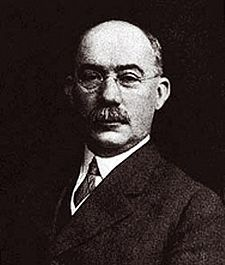
\includegraphics[width=\textwidth]{./graphics/henry-gantt}
\caption{Henry Laurence Gantt, A.B., M.E. (1861 - 23 November 1919) was an American mechanical engineer and management consultant who is most famous for developing the Gantt chart in the 1910s.
These Gantt charts were employed on major infrastructure projects including the Hoover Dam and Interstate highway system and continue to be an important tool in project management.}
\end{marginfigure}


These charts who are produced using Primavera by the Planning Department is
virtually our only tool that communicates the MEP sequence of works to the
rest of the Construction Team. None of the other methods that we have 
discussed handles this intercommunication. During construction though
experienced Construction Managers would normally revert to simpler tabular
or visual methods.

A simple gantt chart (more of a bar chart) can be used to define longer period
activities, that can establish targets. This does not show interdependencies
of activities and for which a more complicated version should be prepared by
the Project Planner. It is important also to bear in mind that if the works 
are delayed for reasons other than owr own (i.e., for example by late information
or by changes) unless there is a good document illustrating these delays it is
extremely difficult to justify the delays.


\begin{fullwidth}
\begin{figure*}[htbp]
\newcommand{\gbar}[3]{\ganttbar[crosshatch, color=orange]{#1}{#2}{#3}}

\definecolor{lightgray}{rgb}{0.7,0.7,0.7}
%% #1 11 rows deep
%% #2 24 cells wide

%% Define short-cuts for months
%%


\def\gantscale#1{}

\newcounter{acount}
\setcounter{acount}{0}
\stepcounter{acount}
\addtocounter{acount}{10}



%\ifnum\theacount>10 number is greater than ten \else number is less than ten\fi


%% Define the months just in case they have not been set
%% before. This needs to be internationalized.
\def\mon#1{\ifcase#1\or%
  Jan\or Feb\or Mar\or Apr\or May\or Jun\or%
  Jul\or Aug\or Sept\or Oct\or Nov\or Dec\else Error 
\fi}


%% a helper macro to add a comma and a space to make the
%% code later on a bit more cleaner

\def\addcomma{, }

%% We define a new counter for looping through the months
%% in order to create the calendar on top
%% this will need to be expanded later 
%\newcounter{monthcount}
%\setcounter{monthcount}{1}
%\whiledo{\value{monthcount}<12}
%  {%
%   \mon{\themonthcount}%
   % adds comma except last one
 %  \ifnum\themonthcount<11 \addcomma\else\relax\fi %
   
  % \stepcounter{monthcount}% 
  %}


%% prints date
%\mon{\numexpr 1+3\relax} \intcalcAdd{\number\year}{1} \relax

%% Global setup
%% 

\xdef\monthstoplot{40}
\xdef\linesdeep{9}

%% Chart drawn in the margins
%% This is the main routine for the chart

%% We define a scale
%
\def\ganttscale#1{#1}



\begin{gantt}[xunitlength=\ganttscale{0.25cm},  fontsize=\footnotesize, drawledgerline=false]{\linesdeep}{\monthstoplot}

%% Define the title of the chart
%%
%% 
\newcommand\GanttTitle[1]{
\ganttitle
    \titleelement{\textsc{#1}}{\monthstoplot}
\endganttitle
}


\GanttTitle{ECU and Black Steel Installation - All Towers}

\begin{ganttitle}
%% We define a new counter for looping through the months
%% in order to create the calendar on top
%% this will need to be expanded later 
\newcounter{monthcount}
\setcounter{monthcount}{1}
\whiledo{\value{monthcount}<11}
  {%
   \mon{\themonthcount}%
   % adds comma except last one
   %\ifnum\themonthcount<11 \addcomma\else\relax\fi %
   \titleelement{\mon{\themonthcount}}{4}
   \stepcounter{monthcount}% 
  }
 
\end{ganttitle}

%% We now loop to typeset the week labels
%% this needs to become more sophisticated
%% as some months do not have 4 weeks
\begin{ganttitle}
   \newcounter{weekcount}
   \setcounter{weekcount}{1}
   \whiledo{\value{weekcount}<11}
  {%
   \mon{\theweekcount}%
   \numtitle{1}{1}{4}{1}
   \stepcounter{weekcount}% 
  }      
\end{ganttitle}
 
%% We define some new colors
\definecolor{red}{rgb}{1,0,0}
% activities are plotted here
\xdef\prop{crosshatch, color=orange}

\ganttbar[\prop]{Rotana }{0}{14}
\ganttbar[crosshatch, color=gray]{Rotana - commissioning}{15}{6}


\ganttbar[crosshatch, color=DarkGreen]{Shangrila}{4}{14}
\ganttbar[crosshatch, color=gray]{Shangrila - commissioning}{19}{6}



\ganttbar[crosshatch, color=DarkGreen]{Merweb}{18}{6}
\ganttbar[crosshatch, color=Gray]{Merweb - commissioning}{24}{3}

\end{gantt}

\caption{All three Towers ECU and black steel installation and commissioning program. Planning provides a safety factor for all Towers for more than two months. We have also allowed for a longer than normal commissioning period in case we are faced with unforseen problems during commissioning.}
\label{plan}
\end{figure*}

\end{fullwidth}



%   
%\section{The gantt package}
%
%In the following you will find a short description of environments and commands: 
%
%The gantt environment draws the canvas of a gantt figure (realized as tikzpicture)
%The usage is |begin{gantt}[...]{no of Tasks to plot}{no of time slots}|
%The optional argument |[...]| can be filled in a |key=value| syntax, using one or more of the following keys:
%
%\begin{description}
%\item [xunitlength]  length of one time slot (default: 1 cm)
%\item [fontsize] fontsize of labels (default: |\normalsize|)
%\item [titlefontsize] fontsize of title section (default: |\small|)
%\item [drawledgerline] Switch to enable/disable the drawing of horizontal ledger lines (default value: false)
%\item [ganttitle] is the environment for drawing the title section
%\item [titleelement] draws one element of the title
%usage: |\titleelement{label}{length}}|
%\end{description}
%
%
%
%
%The \cmd{numtitle} draws a numbered sequence of title elements:
%usage: 
%
%\begin{teX}
%\numtitle{start number}{increment}{end number}{length of each title element}
%\end{teX}
%
%\cmd{ganttbar} draws a single, unconnected bar for representing a task
%usage: 
%
%\begin{teX}
%\ganttbar[pattern]{label}{start}{length}
%\end{teX}
%
%where the optional pattern argument is a tikz pattern, nice patterns for tasks are: 
%north west lines (default), north east lines, crosshatch, crosshatch dots, grid, ...
%
%
%\begin{verbatim}
%\cmd{ganttcon} draws an arrow between to bars with specified coordinates
%usage: \ganttbar{startx}{starty}{endx}{endy}
%
%\ganttbarcon draws a single bar \textit{and} connects the bar with the previous bar for consecutive tasks
%usage: 
%
%\begin{teX}
%\ganttbar[pattern]{label}{start}{length}
%\end{teX}
%
%where the optional pattern argument is a tikz pattern, nice patterns for tasks are: north west lines (default), north east lines, crosshatch, crosshatch dots, grid.
%
%\ganttgroup draws a bar to group tasks
%usage: \ganttgroup{label}{start}{length}
%
%\end{verbatim}
%\section{Physical completion}

%\label{g:test}
%
%\numberLineAt{10}
%\begin{teX}
%\def\mon#1{\ifcase#1\or%
%  Jan\or Feb\or Mar\or Apr\or May\or Jun\or%
%  Jul\or Aug\or Sept\or Oct\or Nov\or Dec\else Error 
%\fi}
%\end{teX}











%These are notes for the gantt chart


\section*{Responsibilities}

Planning spans across all lines of management. Table indicates the type of plans
required and who is responsible to produce them.

\begin{tabular}{lllll}
\toprule
item  &Description            &Prepare   &Check &Approve \\
\midrule
1 &Project Plan               &Planner   &PMs   &Pro. Director\\
2 &6-week look aheads         &Section eng. &PM  &--\\ 
3 &Graphical monitoring plans &Section Eng. &PM  &--\\
4 &Drawings Planning          &CAD Manager  &DM  &PD\\
5 &Materials Planning         &MCD Manager  &PM  &PD\\
6 &Mobilization/demobilization &Planner     &HR  &PD\\
7 &Documentation Plan         &Planner      &DM  &PD\\
8 &Claims                     &Comm.Manager &    &PD\\
\bottomrule
\end{tabular}


\section*{Delays}

Delays and changes to planning are inevitable. As you will recall one of the main 
purpose for developing plans in the first place is to be able to estimate and predict
the impact of events on the end date of the Project. It is the responsibility of the 
Engineer in charge and the Project Manager to identify these delays and appropriate
action be taken to mitigate them, either by requesting more resources to accelerate
the works - once the constraints are removed - or by requesting for an extension
of time.


























\chapter{Engineering}

In our line of work \textit{design} is both ill-defined as well as generally poorly
misunderstood and applied. On most Projects the Owner would have appointed a
Consultant who will produce a design and give it out to tender. In many cases
this is incomplete and supplemented with every conceivable type of clause in a
specification to limit claims by the Contractor. On other type of Contracts we
might have design responsibility for the full works. These are called design-build contracts. In either case a substantial amount of engineering needs to be developed
to complete the design, procure the materials, install the works and putting the
plant into operation.



\section*{The Engineering Department}

On Projects that are not design-build an Engineering Department is set-up with
an Engineering Manager. He is normally assisted with Design Engineers. In addition
he is the ultimate responsible person for overseeing the works of the CAD Office.

\section{Design Audit}

At the start of the Project a quick design audit is undertaken to review the
current design by the Engineer and to identify areas of concerns, missing information and opportunities for savings in costs. This should be summarized in a report with
full details. The same document can then progressively be modified to record all
changes and calculations as works progress.

\subsection*{Selection of equipment}

Equipment selections and submittals fall within the work that the Engineering Department undertakes. As these works might take time to implement the Project Director at the early stages of a Project allocate responsibilities to Senior
Engineers to assist. Some equipment might need calculations before they are ordered as for example fans, pumps, cables, electrical boards and similar items.


\section*{Drawings}

The production of drawings should be done in the \textit{fastest} way possible. 
This is important for two reasons:

\begin{enumerate}
\item As at the beginning of the Project, information might be missing, this is
the best time to record delays, before any \textit{concurrent delays} occur. In many instances the Project Managers or Engineer might issue an information schedule, i.e, a time table listing all the missing information and when this will be issued. Unless this is covered with the Clause (14) programme, one should only accept with the reservation that the Contractot has a right to claim for late information. The Commercial Manager for certain would need to respond. Although
late information for sanitary fixings might not delay the Project it may delay the
drawings and the opening required to accommodate floor mounted units and similar items. If the Engineer has issued a set of IFC drawings no further delays without claims would be acceptable.
\item If works start late on site due to late issue of Shop Drawings or unavailabilty of materials due to late issue of information we would need to add
tradesment to accelerate the works and keep up with the programme. It is always easier to add one CAD Operator than to add 100 tradesmen and more cost effective, given the inefficiencies of disruption and crowded work faces.

\end{enumerate}

\section*{How big a team}

Although, this will depend on the quality of the original design, the number of services involved, the nature of the Project and if the Building has areas where
the design is repetitive a good formula to use is the following:

\begin{equation} n = \sum_{n=1}^{n=k}\frac{f_1}{100}\times C + \frac{f_2}{100}\times C +\cdots+\frac{f_k}{100}\times C_k
\end{equation}

The mimimum size Team should never be less than 16 on Projects that are greater
than QR~200~million.



\section*{Co-ordination}


Possibly more than 70\% of all issues that cause work to stop or to move 
inefficiently can be attributed to poor co-ordination. Although the original
designers bear responsibility for primary co-ordination, we bear responsibility
for co-ordinating the services and for raising the alarm when there are problems
with primary co-ordination.
\begin{marginfigure}
\tikz
\node [forbidden sign,line width=1ex,draw=red,fill=white, scale=2.0] {CLASHES};
\end{marginfigure}

\subsection*{Co-ordination sequence}
At the start of a Project co-ordination needs to follow a sequence of works and
although one will need to go through a number of iterations before the drawings
can be finalized the following sequence will work in most typical cases:

\begin{enumerate}
\item If the ceiling voids have large beams, consider locating the fire mains within the
void provided by the beams to conserve space. Fire mains can easily be sleeved
through and is a good solution, especially in car parks.
\item Drainage pipes should be located hard against the nearest beam and sloped as required, consider changing direction if necessary to have drainage pipes run
shorter routes.
\item It is normal where there is drainage pipes to have cold and hot water. Following a similar route for these pipes would ease co-ordination. 

\item Cable trays should be similarly zoned in parallel with walls. Preferably
no other services should run under or over cable trays to enable clearances for 
pulling cables.

\item Ductwork is a special case and if possible should be run at the lowest level
with flexibles \textit{on the side of the ducts}.

\end{enumerate}

\subsection*{Co-ordination in shafts}

\begin{enumerate}
\item Shaft co-ordination should start early and if possible the first type of co-ordination to take place. This is important as any crossover of services
would seriously reduce ceiling void heights.
\item Always consider providing a platform in shafts. Although this might marginally add to costs, it can speed-up construction tremendously and enable easy hoisting of piping through the shafts.
\item Method of accessible shafts, need to be agreed with stakeholders.
\item For typical plumbing shafts on high rise buildings and or hotels and
apartments consider making an early mock-up--not necessarily in situ--to 
optimize the installation and work out small details such as expansion.
\item Allow adequate space behind ducts and pipes for access to install insulation. This is a normally an overlooked aspect.
\end{enumerate}


\subsection*{Co-ordinators}

Each CAD operator has responsibilty to check his work in terms of
completeness and co-ordination.

\subsection*{Common pitfalls}

\begin{enumerate}
\item One service obstructing another, such as a BMS control box installed too near a fan-coil unit, so that it cannot be opened. This is also common with MCC
boards being too big and cannot be accomodated in Plantrooms.

\item Condensate drains on mechanical equipment that have been - missed on drainage drawings. This can be avoided by showing condensate drains and fan-coil
units on a separate layer and importing this layer on both the VAC drawings
as well as the drainage drawings. Similarly for any equipment requiring power supplies etc.

\item Not allowing an adequate clearance both under or over sectional water tanks.
		This is also a common error by Consultants.

\item Very low plinths for AHUs with high static pressures. This can also happen
		when plinths are designed from structural drawings and then waterproofing is about
		50 mm high ending up with plinths that are only 50 mm high. 

\item Not allowing properly for the curvature of cables when entering switchboards
		or for panels to be ordered bottom entry but the cables are top entry. This is a 
		result of poor scheduling and detailing.

\end{enumerate}



\section*{Professional Drawings}

One can easily recognize a professional drawing when he sees one, but it is 
very difficult to explain what makes a drawing professional.
These are some parameters:

\begin{enumerate}
\item All information required to execute the works is shown on the drawings.
\item Details are specific for the Project and are meaningful.
\item Schedules.
\item Cross referencing.
\item Good choice of pens and styles.
\item The drawing has \textit{dimensions}. 
\item The drawings include sections and larger scale details.
\item The drawing is printed at the right scale.
\end{enumerate}















\chapter{Site Works}

\epigraph{In most people’s vocabularies, design means veneer. It’s interior decorating. It’s the fabric of the curtains and the sofa. But to me, nothing could be further from the meaning of design. Design is the fundamental soul of a man-made creation that ends up expressing itself in successive outer layers of the product or service.}{Steve Jobs}

Siteworks encompass the actual construction. Everything we do is immaterial
unless the works on site can be executed.

\section*{Responsibilities}

Any works on site fall under the responsibility of the relevant Section Engineers.
The Project Manager will manage his section\sidenote{A section of the works
is not necessarily defined by area, but it can also be defined by service for example drainage works will normally fall onto one or two section Engineers, whereas another one might be responsible for a Tower.} of the works but ultimately
the owner of a section of the works is the Project or Site Engineer.


\section*{Resource Scheduling}

The Section Engineer is responsible to plan, monitor the execution of the works
and produce daily and weekly reports as required.

\section*{Workflow}

All Section Engineers and as a matter of fact everyone working on the Project
must be familiar with the standards required of the Project by having read the
specification and by having studied the drawings of his section.

On having been allocated a section of the works the Section Engineer needs to
complete the following activities:

\begin{enumerate}
\item \textit{Review Shop Drawings} One needs to take into consideration that
 Shop drawings might not contain the full information required to carry out the works. The Section Engineer must review the drawings carefully, assist if necessary
with comments that will enable further details to be added and that co-ordination
is possible, ceiling heights achievable and shafts workable.

\item Keep a set of drawings for red-marking.
\item Create a Materials Plan.
\item Prepare Material Take-offs.
\item Issue Site Order Releases.
\item Liaise with Main Contractor for Civil works.
\end{enumerate}


In many instances due to Projects peaking at different times, it is quite likely
that an Engineer will be allocated to a Project during a period that the works
are under pressure. This should not really matter, but then it is still the Section
Engineer's responsibility to make sure that the above steps are followed. If he
is replacing someone that has left the Project then if there is a handover report 
one can verify that the information is correct.

\section*{Site Diary}

All Section Engineer's should keep a Site Diary in which to record the day to
day activities of the works. The Site Diary can be invaluable if claims are
lodged and eventually there is arbitration. The minimum information that must
be logged is:

Area and type of works : start date/end date.

Personnel allocation.

Problems encountered.

Key events related to milestones.

In general keep as much information as possible to enable someone - with your
assistance to recreate the events during the construction period.
\begin{marginfigure}
\includegraphics[width=\textwidth]{./graphics/abandoned-materials}
\caption{Abandoned and dirty materials, make for a very unprofessional work place.}
\end{marginfigure}
\section*{Workface Housekeeping}

There is nothing more wasteful than materials and waste lying all over the
place. The section Engineer must set daily procedures and responsibilities
to ensure that all workfaces are clean, even if this entails cleaning
some of the Main Contractor's rubble that was left behind, when they arrived
and made opening that we \textit{forgot} to tell them about. By keeping the
area clean you ensure that not only it is safe to work but waste is
eliminated and productivity improves. Have an adequate supply of clear plastic
bags for the disposal of rubbish (use clear bags to minimize pilferage).


\section*{Protecting the works}
You should ensure that the works are always protected. All piping and ducting should be wrapped in polyethylene when completed and all open ends closed to minimize the amount of debri and dust that can get in. This ensures that
during commissioning less time is spent in cleaning the system. 


\section*{Damage Reports}

However, hard you try at a point you will reach a stage at which some damages
would occur. These are reported properly using a Damages Report format, which
is issued via the Commercial Department as a claim. Be certain that at the
end of the Project you will face the same from other parties. A damaged works
log is to be kept by the QA/QC Department, as well as Document Control.




\section*{Quality}

Although quality assurance and quality control are handled in a dedicated chapter
we have to mention it here. The Section Engineer is resposnible for the quality
of the works in his area. It takes the same effort to complete the works with the right quality as substandard work. In general the following strategy works
well in raising the bar on quality:

\begin{enumerate}
\item Never accept substandard work
\item Prepare a prototype for all works that you are starting for the 
 first time. This will ensure that all stake-holders and technicians understand
the quality of works required.
\item Offer constructive advise to technicians and supervisors during your
Site Walks for work that just does not look right.
\item Snag the works before you  offer them for inspection.
\item Attend the inspections (if not all of them) at least the ones that 
are offered for the first time or that have failed and are offered again for
inspection.
\item Do not offer works for inspection unless you have checked and can verify
that all materials used are as per approved submittals and the installation is as
per approved drawings. Essentially you must make sure that the materials are
correct and the installation is as per the contract, which in most cases is as
per specification and drawings. Investigate any deviations and take remedial
action if necessary.
\end{enumerate}


\begin{marginfigure}
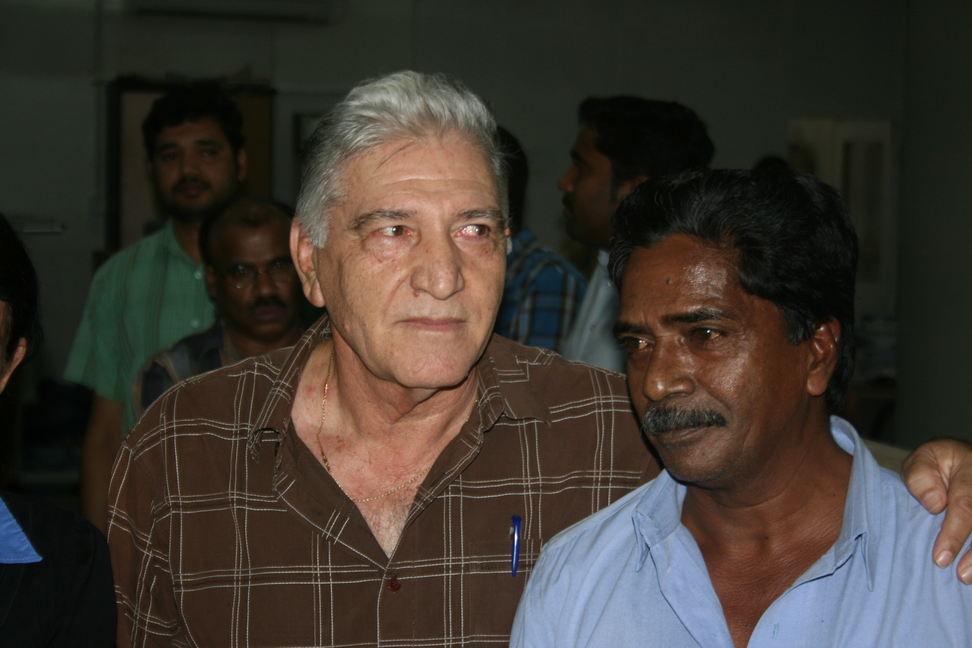
\includegraphics[width=\textwidth]{./graphics/team-spirit}
\caption{Create an environment of openess and co-operation. Quality and targets
are only achieved via a spirit co-operation and Team Work.}
\end{marginfigure}
\subsection*{Quality perception}

Most inspections are \textit{visual} and hence perception psychology plays
an important part. A well lit and \textit{clean} area  with a Team on standby that looks professional, with you having done your homework so that you can answer any question that the
inspector asks will go a long way to a trouble free inspections. With over
30,000 inspections budgeted on larger Projects, if you do not take care of
inspections they are bound to cause delays. 

Other visual items that you will need to take care of is paintwork, supports,
slopes of piping and insulation. 

\begin{marginfigure}
\includegraphics[width=\textwidth]{./graphics/fire-pipes}
\caption{Painted and cleaned piping works and ensuring that nearby pipes run at the same level increase the perception of quality and makes work look professional.}
\end{marginfigure}


\subsection*{Low quality}
If you find that quality is consistently below an acceptable level, make sure 
that you arrange for training for the concerned technicians and or have a prep
talk with everyone. Discuss it with your senior Supervisor and decide what to do.

\section*{Ensure everything will work}

While the daily pressures of work force Engineers to focus on their own section
of works, keep an eye and an enquiry mind to make sure everything works. You 
are the last safety net of both the professional as well as the Contracting Team
to pick up and problems that have not been seen earlier. Ask yourself, will
it work, what happens when something is switched on, can we drain this section
of the works, does it need another valve and so on. You also need to think about
being able to access works for maintenance and also for balancing. So if you have
an access door on a duct taht you cannot open because there is a sprinkler pipe
running across it, you need to take care of it. In general, in this part of the
world, it will cost more to add temporary flushing loops and drains, so ensure
that these have been marked on drawings or take action to request that they are
shown on drawings.




































































\chapter{Quality Assurance and Quality Control}

Quality cannot be accurately defined, but you know it when you see it. On a Site
Quality is the responsibility of everyone and it generally means that you need to
give attention to details.

\section*{The steps to quality}

There are a number of steps that you need to take in order for your work to
be considered quality work and they are really simple.

\begin{enumerate}
\item  Define what you need to do and how to do it. Although the definition part
is simple, it needs to meet the specification, in reality in most cases the specification may be vague. You define the product by making a prototype and by ensuring that it is correct from all angles.

\item Add repeatabiliy

\item Cleanliness

\item Presentation

\end{enumerate}

\section*{The paperwork}

There is a lot of paperwork involved with QA/QC Departments, as a matter of fact perhaps not enough paperwork on a MEP Site as compared to say a manufacturing plant.
\chapter{Communication}

As a rule the medium of communication for Engineers is \textit{drawings}. Engineering is a highly complex field, is information dense and difficult to transmit ideas non-visually. You can have a specification which is six pages long for an example a cooling tower. On a Drawing a simple drawing can describe all that information in a more concise and clear way.

Many other items can be described in traditional documents use in construction:

\begin{figure}
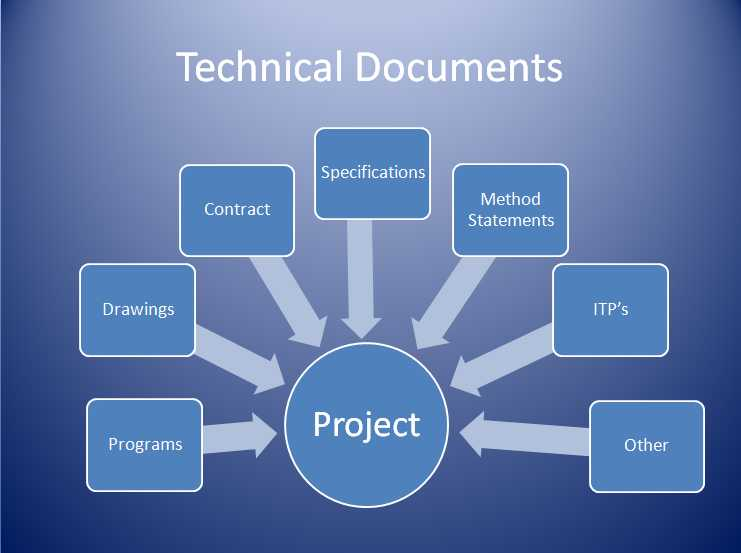
\includegraphics[width=\textwidth]{./graphics/process-02}
\end{figure}

What materials are we going to Supply? This is communicated through technical submittals.

How are we going to install them and test them? This is communicate through ITP's and Method Statements.

When are we going to carry out the work? This is communicated through a Programme of Works.

Who is doing What? This is normally through our organization charts?

Many a better head than this writers have found ways to manage projects along these documents. Although sometimes when misused can cause undue delays, the absence of them can lead to a disastrous Project.

Engineers are not good communicators in general, they work long hours and under pressure making communication more difficult. Try and put as much information on
a drawing as possible. Remember they used to be called plans.


In general we try to commuicate with documents. By utilizing documents rather than verbally communicating requests, actions and the like, documents can flow better. In general use the phone, if you can achieve what you want with the phone-call (such as obtaing the status for something). If the action you request from the person who is next on line will only be completed after a few days commuicate in writing.

\subsection*{Follow-ups}

A message flows better between two people rather than a number of persons. In designing our processes we have kept that in mind. As a rule of thumb if you need to follow-up on a particular action, you need to do it with the person you have send the document to. As an example you have send a request for a purchase. It is no good phoning the Area Manager iff he had approved it or the Financial Department if he has issued the check. You need to follow with the Department head to whom you have addressed the documents. (He might have just finished a meeting with the Financial Manager and a direct call to Accounts, in a way will relieve the MCD Department of his responsibility to expedite)!

\begin{figure}
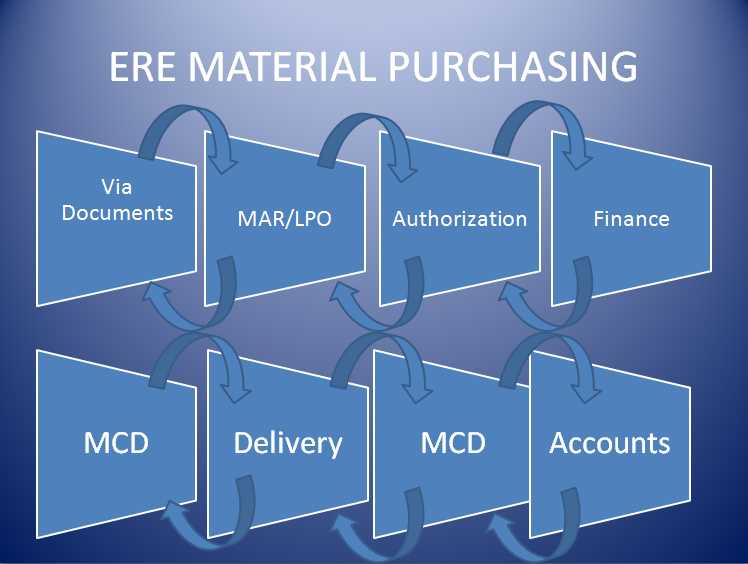
\includegraphics[width=\textwidth]{./graphics/process-01}
\end{figure}

\subsection*{External communications}

Our philosophy is to strive and be professional with our interactions with other Companies. In general we will take a non-confrontational attitude that is pro-active and logical. This does not mean however that we will not stand for our rights.

\subsection*{Documentation}

All documentation with external Companies should be in writing. Either being our own suppiers and sub-contractors or the Client and other members of the professional team. Special care should be taken in approval of variation orders, invoices and other similar issues to our sub-contractors.
\chapter{Contractual}

It is important that all Engineers are aware of the original scope of works. The original scope of works can be found here.

Responsibility for raising the issue of V.O.'s is as follows:

\begin{figure}
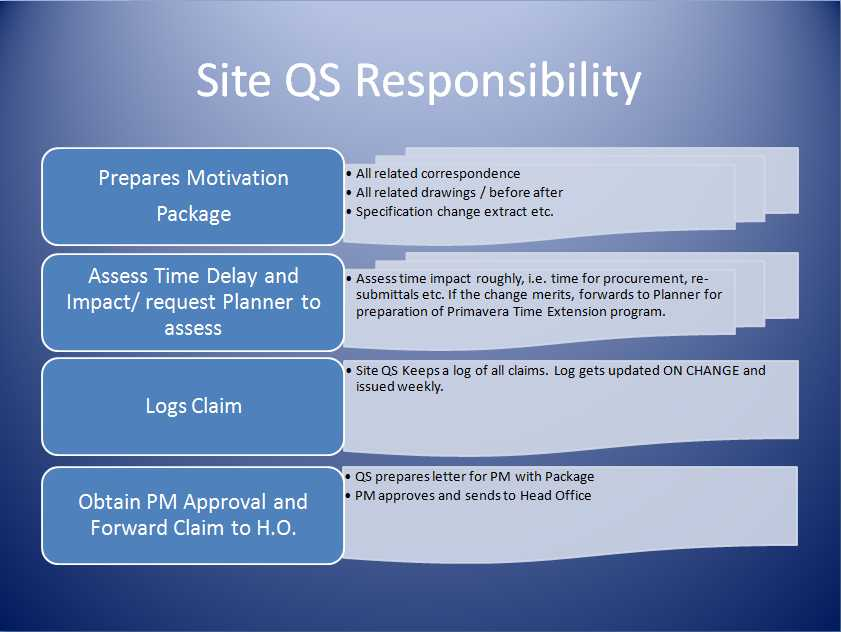
\includegraphics[width=1.3\textwidth]{./graphics/Site-QS-responsibilities}
\end{figure}


It is a very rare occassion that the person originating the change will
issue an instruction and a variation without us asking for it. However,
small this request is, being professional and recording the change will
ensure that in the event that all these minor variations add up, a proper claim
can be lodged.

\section*{Variation Orders}

\subsection*{Awareness}

\begin{tabular}{|l|l|p{2.0cm}|p{2.0cm}|p{2.0cm}|}
\hline
Person &Design Changes&Change via EI, RFI or Letter&Program Changes&Verbal Site Instructions\\\hline
Project Manager    &X&X&X&X\\\hline
Engineering Manager&X& & & \\\hline
Senior Engineers   &X&X& & \\\hline  
Site Engineers     & & & &X\\\hline
Supervisors        & & & &X\\\hline
Planner            & & &X& \\\hline
\end{tabular}  

\section*{Engineers Instructions}

In order to be able to submit a variation as per our contrcat with ADCC and following common practice an Engineers Instruction or otherwise needs to be issued to us. The ONUS is on us to request it.

Copies of Engineers Instructions are sent to H.O. Attention: Mr Fiaz who will then monitor and ensure that it is submitted.

\section*{Site Responsibility}

To issue adequate backgound information for the Variation Order to be submitted. This shold include the `narrative' as well as any other back-up documents.


\section*{Issuing}

All documents to flow through document control. All distribution through document control.

\begin{figure}
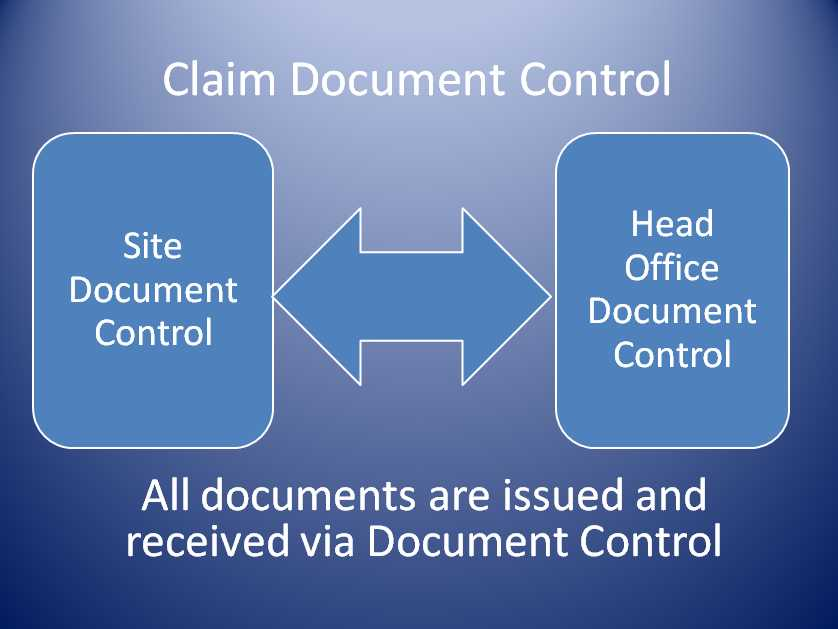
\includegraphics[width=1.3\textwidth]{./graphics/document-control-01}
\end{figure}


\section*{Impact of change orders}

The chart below show the impact of change orders and their distribution. 

\begin{figure}
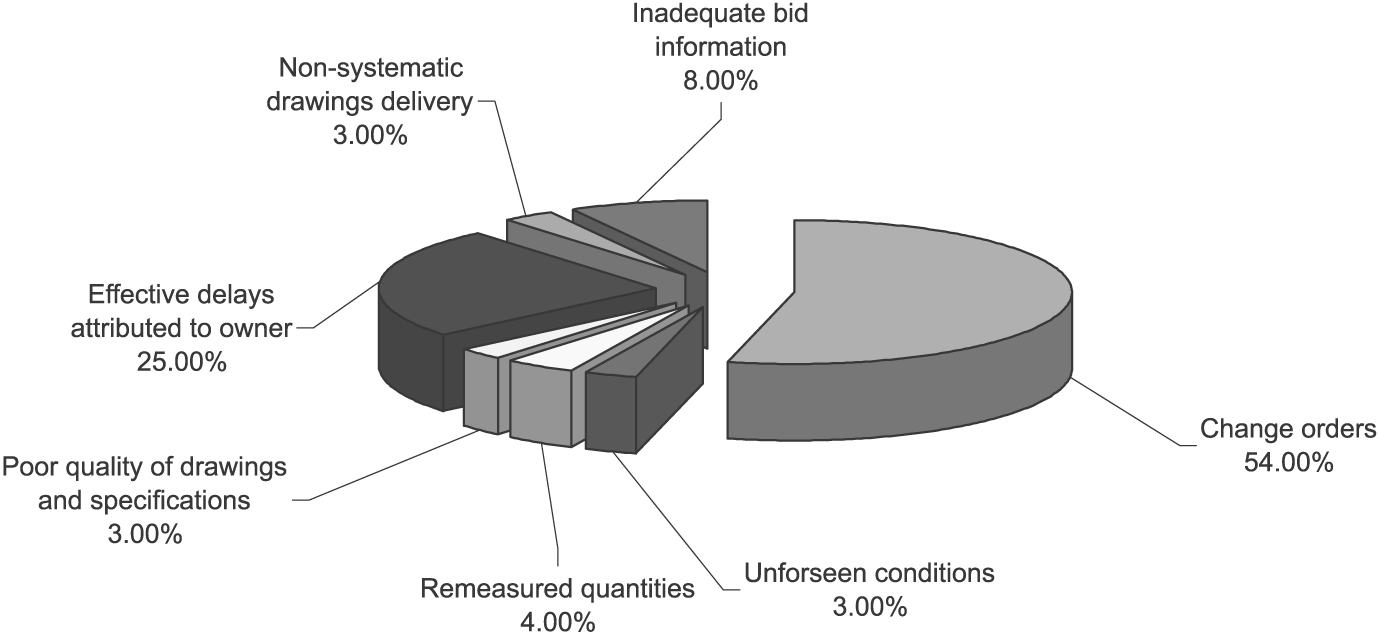
\includegraphics[width=1.3\textwidth]{./graphics/change-orders}
\end{figure}

On Projects where we expect numerous changes we prepare \textit{measle charts}  or
as we call the \textit{chicken pox diagrams}. Like a person afflicted with the
disease your work will be slowed down and the cumulative impact will be much
greater than you think.


\begin{fullwidth}
\begin{figure*}
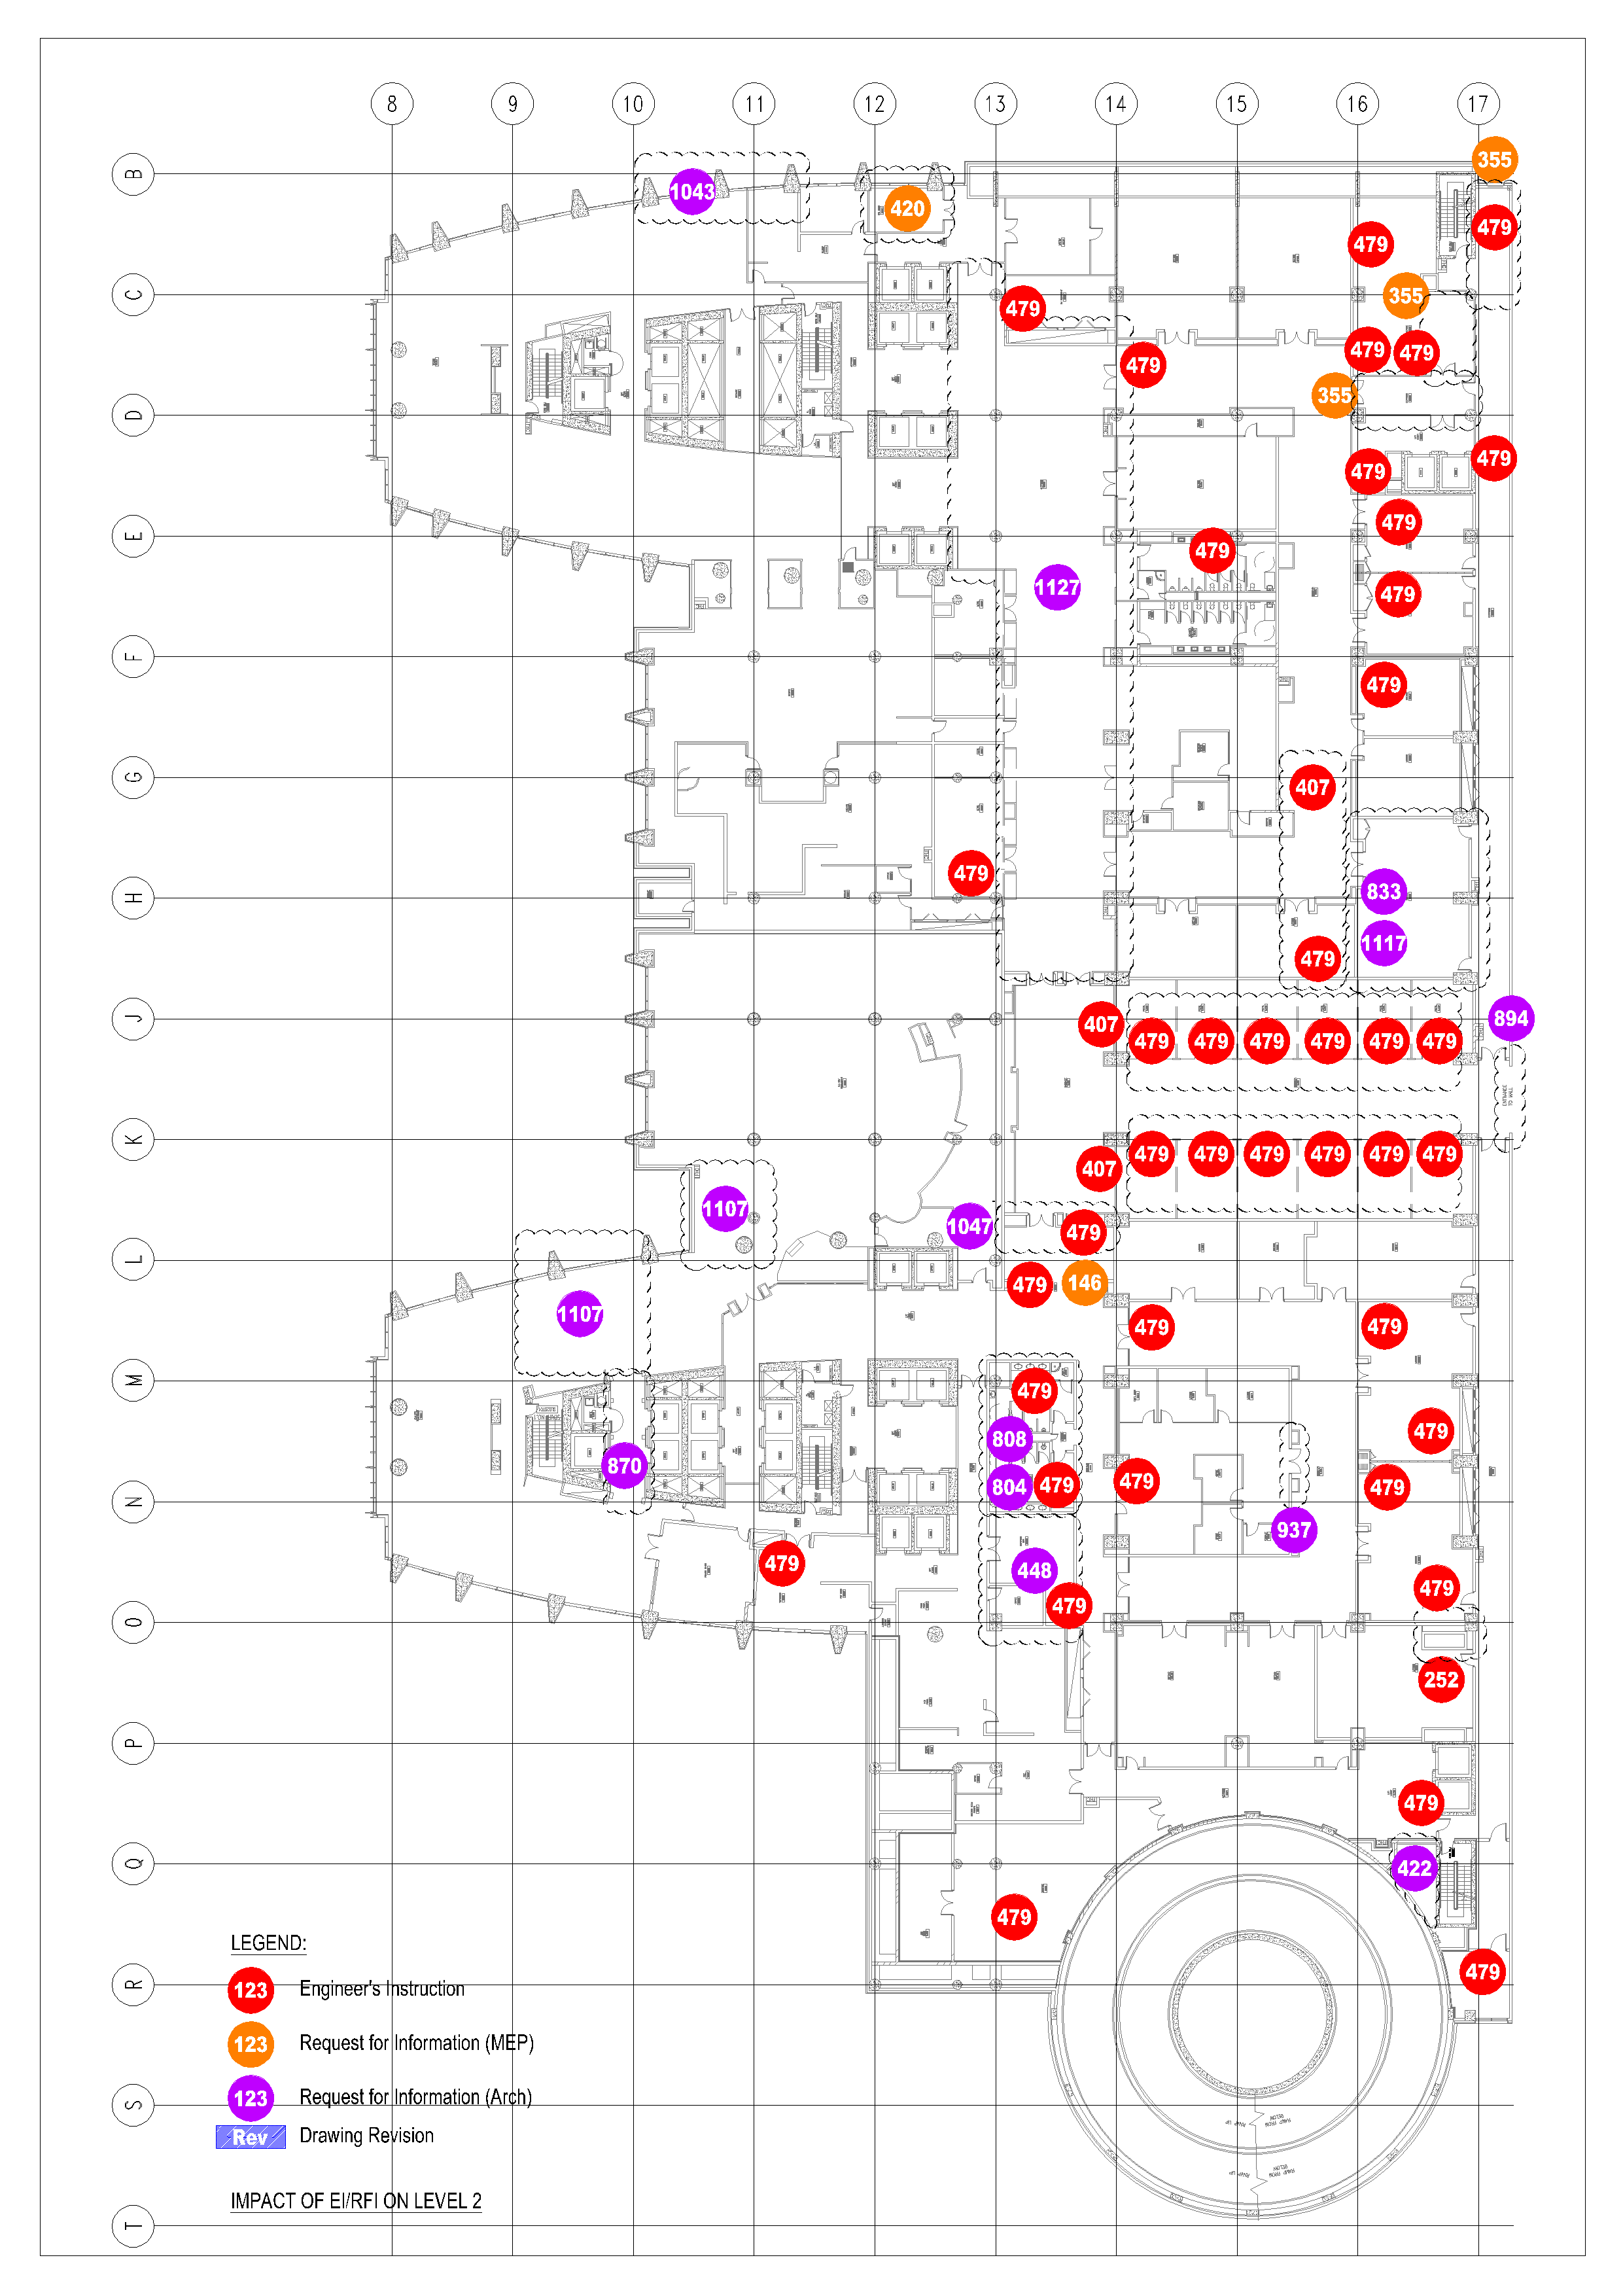
\includegraphics[width=1.1\textwidth]{./graphics/AHU/cpL2}
\caption{Chicken pox diagram showing effect of EIs and major RFIs on a Project.}
\end{figure*}
\end{fullwidth}

\section*{Recording the changes}

Once a Change Order is initiated a number of steps need to be taken
to ensure that contemporaneous records are kept.

The Site QS needs to ensure that a letter is dispatched recording the fact
that the change order will have a time and a cost impact.

The Engineering Manager will need to ensure that the Change Order is reflected
permanently on drawings. The Shop Drawings need to be revised. Please ensure
that revision clouds are included and that the revision text clearly states
the reason for the change.

The Project Manager and Section Engineers will need to assess the impact of
the EI and inform the Commercial Manager of the impact.

The QS will produce weekly and monthly reports as well as record on the
monthly valuations the impact.

\begin{fullwidth}
\begin{table}[htbp]
\vspace{1cm}
\small
\begin{tabular}{l c c c c c c c c c c c c c c c c c c c}
\toprule
~ &Dec & Jan & Feb & Mar & Apr& May & Jun & Jul & Aug & Sep &Oct & Nov &Dec &Jan & Feb  & Total\\
~ &09  & 10  & 10  & 10  & 10 & 10  & 10  & 10  & 10  & 10  &10  & 10   &10 &11&11&11 \\
\midrule
Phase 3a &17 &9 &10 &17 &9 &21 &12 &15 &16 &13 &15 &15 &7 &6&6&187\\
Phase 3b &1   &3 &0 &3 &2 &5 &0 &3 &3 &1 &3 &11 &4 &6&nil&46\\
\midrule
Phase 2a$+$3b &18 &12 &10 &20 &11 &26 &12 &18 &19 &14 &18 &26 &11 &12&16&233\\

\bottomrule
\end{tabular}
\hskip-10cm\caption{Total number of EIs received since the MOU}
\label{tbl:EI}
\end{table}
\end{fullwidth}

\begin{fullwidth}
\begin{table}[htbp]
\vspace{1cm}
\small
\begin{tabular}{l c c c c c c c c c c c c c c c c c c c}
\toprule
~ &Dec & Jan & Feb & Mar & Apr& May & Jun & Jul & Aug & Sep &Oct & Nov  & Dec & Jan & Feb & Total\\
~ &09  & 10  & 10  & 10  & 10 & 10  & 10  & 10  & 10  & 10  &10  & 10   &10 &11 & 11& 11\\
\midrule
Phase 3a &34  & 38  & 63  & 51  & 56 & 50  & 51  & 79  & 32  & 36  &32  & 41   &31&38&17&661 \\
Phase 3b &12 &19 &12 &7 &28 &24 &23 &21 &5 &8 &12 &13 &5&6&7&204\\
\midrule
Phase 2a$+$3b &46 &57 &75 &58 &84 &74 &74 &100 &37 &44 &44 &54 &36&44&24&865\\

\bottomrule
\end{tabular}
\caption{Total number of RFIs issued since the MOU}
\label{tbl:RFI}
\end{table}
\end{fullwidth}


Charts can assist to better visualize problems with Engineer's Instructions
and RFIs.

\chapter{Cumulative Impact of other EIs and RFIs}
\newthought{A growing list of Engineer's Instructions and Requests for Information} followed-up, the signing of the Memorandum of Agreement. The growth of the EIs is shown graphically in Figure~\ref{EIplots}. As at the end of May 2011, there were 300 EIs issued and 1054 RFIs.
Not only the Engineer failed to complete his design by the 15th of December 2009, as agreed with the Contractor and recorded in the Contractor's approved 6.2 Programme of Works, but the Engineer continued with changes well into a year after the planned Completion Date.


\def\monthnames{{"D","J","F","M","A","M","J","J","A","S","O","N","D"}}
\pgfplotsset{width=16cm}

\begin{fullwidth}
\begin{figure*}[htbp]
\begin{tikzpicture}
    \begin{axis}[
        smooth,
        stack plots=y,
        area style,
        enlarge x limits=false,
        ymin=0,ymax=1500,
        xlabel=\textsf{December  2009 to May 2011},
        ylabel=\textsf{Number of Eis and RFIs},
        xtick=data,
        %no need to repeat months more than a year
        xticklabel={\pgfmathparse{\monthnames[Mod(\tick-1,12)]}\pgfmathresult}]
\addplot[color=orange,fill=orange!60] coordinates
		{(0,0) (1,52) (2,103) (3,178) (4,236) (5,320) (6,394)%
                (7,469) (8,569) (9,606) (10,650) (11,695) (12,752)%
                (13,788) (14,833)  (15,881) (16,946) (17,996) (18,1041)
               } 
		\closedcycle;
	\addplot[color=orange,fill=orange] coordinates
		{(0,0) (1,21) (2,32) (3,45) (4,66) (5,78) (6,106)%
                (7,120) (8,138) (9,157) (10,173) (11, 196) (12,223)%
               (13,233) (14,248) (15,262) (16,273) (17,284) (18,299)
               }
		\closedcycle;
    \addlegendentry{\textsf{Requests for Information}}
    \addlegendentry{\textsf{Engineer's Instructions}}
    
   
 
    \end{axis}
\end{tikzpicture}
\caption{Plots showing the growth of Engineer's Instructions and their relationship to Requests for Information, the relationship can be observed clearly. See for example the \textit{bumps} at around April-May 2010.}
\label{EIplots}
\end{figure*}
\end{fullwidth}

No Project, where the Design is incomplete can be completed. It is obvious neither the Owner that could instruct the Engineer to add resources to his Team, nor the Engineer considered the Completion Date to be of \textit{essence}.

The Contractor on its part, accelerated works in sections that were critical for the Owners Direct Contractor to have access, providing this access at the end of June 2010.

% start tikzpicture,define styles
% define a style called activity
\tikzstyle{activity}=[draw,
                      rectangle,
                      rounded corners, 
                      fill=black!5,
                      thick,
                      minimum width=2.9cm,
                      minimum height=2.2cm, 
                      text width=2.5cm
                      ]
\begin{figure*}
\begin{tikzpicture}[mystylei/.style={draw,ellipse,rounded corners, fill=gray!23,thick,minimum
width=3cm,minimum height=1cm, text width=2.5cm, text centered}]


%start to define nodes relative to each other
\newcommand\addblock[2]{\node[activity, node distance=0] (#1) {\textsc{\textbf{#1}}. \textsf{#2}};\def\temp{#1}}

\def\addblockbelow#1#2{\node[activity] (#1) [below=of \temp] {#1. \textsf{#2}};\draw[->] (\temp) -- (#1);
\def\temp{#1}
}

\addblock{1}{Mark EI or RFI implications on drawings}
\addblockbelow{B}{EM to identify implications}
\addblockbelow{C}{Issue Impact form to CM}
\addblockbelow{D}{Obtains approval for revisions. iterates if necessary.}
\addblockbelow{5}{Obtains approval for revisions. iterates if necessary.}


%%\node[activity] (C) [below=of B] {C. Issue Impact form to CM}; 
%\node[activity] (D) [below=of C] {D. Obtains approval for revisions. iterates if necessary.};

%second column with a bit of a distance
\node[activity,node distance=1.3cm] (E) [right=of 1] {E. Commercial Manager, reviews};  
\node[activity,node distance=1.3cm] (F) [right=of B] {F. Impact Forms};
\node[activity,node distance=1.3cm] (G) [right=of C] {G. issue claim}; 

%% Third column      
\node[activity,node distance=1.3cm] (H)  [right=of E] {H. PM reviews}; 
\node[activity, node distance=1.3cm] (J) [right=of D] {J. Cause, narrative};

\node[activity,node distance=1.3cm] (H1) [right=of F] {H1. Plans the works. Issues stop orders if necessary};

%empty node for the gap in column 2 row 3
  
\node[activity,node distance=1.3cm] (K) [right=of G] {K. Issue Impact Form to CM. Photographic records};       
\node[activity,node distance=1.3cm] (H2) [right=of J] {H2. Arranges materials and installation (WIR)}; 



%connect the nodes
%\draw[->] (1) -- (B);
%\draw[->] (B) -- (C);
%\draw[->] (C) -- (D);
\draw[->] (E) -- (F);
\draw[->] (F) -- (G);
\draw[->] (G) -- (J);
\draw[->] (C) to [out=360,in=180] (F);
\draw[->] (D) to [out=360,in=199] (F);
\draw[->] (K) to [out=180,in=360] (F);
\draw[->] (H1)-- (K);
\draw[->] (H) -- (H1);
\draw[->] (K) -- (H2);
%\draw[->] (C) -- (K);

\end{tikzpicture}
\caption{Workflow for Engineers Instructions and RFI works. All Departments get involved when there is a Change Order. Evaluate Change Orders as they occur and keep contemporaneous records. }
\end{figure*}







































\chapter{Site Administration}

On most Sites it is necessary to have an administration Department, header by a capable
administrator.

\section{Size of the administration Office}

To function properly the minimum size of the Administration Department is as follows:

\begin{table}
\begin{tabular}{ll}
\toprule
Designation    &Number\\
\midrule
Manager        &1\\
Admin Officer & 1\\
Time Keepers & 2\\
Driver            &1\\
\bottomrule
\end{tabular}
\caption{Minimum size for administration Site Department.}
\end{table}

The size of the Department will ultimtely be determined from the number of personnel working on the size
and can be increased or decreased during the life cycle of the Project. Given the Competitive pricing
this is one area where efficiency is important to keep costs down. 

\section{What does the Department do?}

For most personnel their encounter with the Company face is the Administartion Department. As such
it is important to keep in mind that people are highly demotivated when faced with inefficiencies of 
administration, especially during difficulties in the employess life, such as a death in the family.

So the first and most important function of the administration department is to act as an internal PRO
Department, helping to instill a culture of professionalism and efficiency. Most matters that relate
with personnel except for their technical work are handled by the Administartion Department.

\subsection*{Processing of Routine Documents}

The processing of daily routine stuff such as leave applications, resignations, demobilization and 
mobilization of personnel, time keeping, issuing of general memos, liaising with counter parts and follow up
with HO personnel.

\subsection*{Medical}

The department is repsonsible to make arrangments for the Medical treatment of employees and to keep
statistics in this respect.

\subsection*{Camps}

\subsection*{Transportation}

\subsection*{Disciplinary procedures}

\subsection*{Site Office Management}

If the Site is large enough, it will employ secretarial, office cleaning, photocopying and other personnel that
will come under the Management of the Administration Department.

\subsection{IT Department}

Id teh Site has a lot of computers the IT Technician or PC support Engineer, may also report
to the administartion department.

A back-up plan and disaster recovery will have to be planned by the Project Director and Heads of
Department.

\subsection{Visas, tickets and similar items}

\subsection{Payment of Salaries}

\subsection{Reporting}

Daily reports must be produced for attendance, deployment of personnel.

Weekly reports should provide a summary of the following:

\begin{tabular}{ll}
Man hours worked          &\\
Percent absenteeism       &\\
Total employees on site   &\\
Total employees on leave &\\
\end{tabular}

The actual format of the report will vary from Site to Site and will also vary if the planner is producing 
similar statistics.

Monthly reports will have a similar structure.

\subsection*{Document Control and Filing}

The section shall keep all documents as described earlier for Document Control. In particular the
following must be kept as a minimum:

\begin{tabular}{ll}
Employee files &\\
Weekly reports &\\
Personnel Movement &\\
Internal Memos &\\
Warnings &\\

\subsection*{Key performance Indicators}

Perhaps the best key performance indicator of the Department is that personnel trust that their paperworks have been processed. At City Center project for example having had to rely on an inefficeint HO it was not unknown for personnel to daily visit the Admin Office to enquire about their leave or visa status daily. 

\end{tabular}






















\chapter{Handover}

It is important that all Engineers are aware of the original scope of works. The original scope of works can be found here.

Responsibility for raising the issue of V.O.'s is as follows:

\begin{figure}
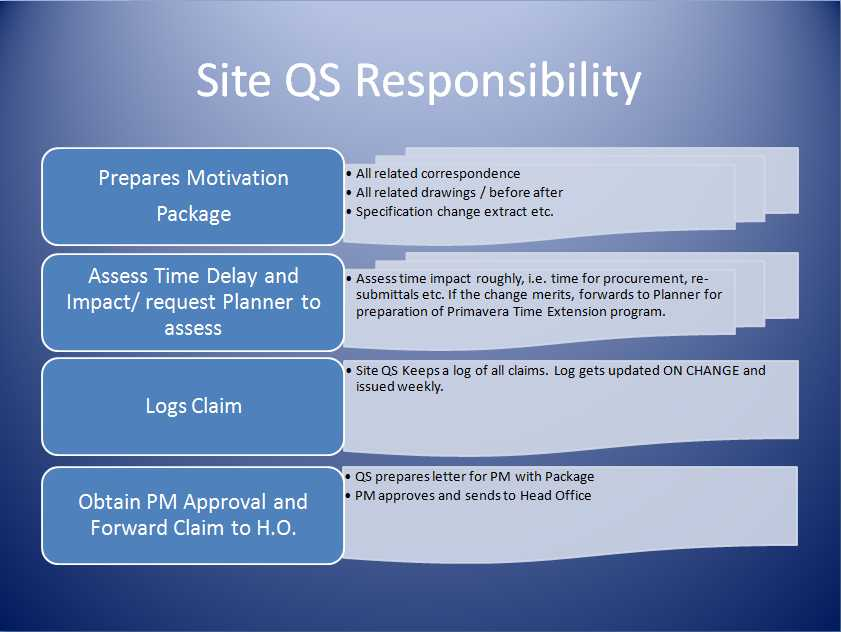
\includegraphics[width=1.3\textwidth]{./graphics/Site-QS-responsibilities}
\end{figure}

\section*{Hand Over Documentation}

The aim of collating all documentation at the end of a Project in order to verify that all parties have inspected and accepted the Installation. These documentation will have to be enclosed in the Operations and Maintenance Manuals.

\section*{As-Build Drawings}

This is the most basic requirements and in an ideal Site they will be produced as an on-going activity, while the Site is operating. Remember that every change on the AS-BUILDS points to lack of good engineering at the beginning of the Project and to an extent lack of planning. Minor changes are understandable to incorporate Site instructions but any large scale operations to update drawings is as a sad story.

\section*{Proof that the Works have been Physically Inspected}

A list of all WIR's properly collated should be summarized.
Contractor's confirmation that the works have been completed.

\section*{Proof of commissioning}


\section*{The Final Touch}

Depending on the specification, the Designers might have even elected to
specify the font and the font-sizes for the manual. The OM manuals will
impact on our brand long after we have left the project. It is important that
they look professional and that they are bound correctly. Drawings and CDs
should be copied properly.











\chapter{Business edge}

\section*{Introduction}

In order to build a business edge we need to define the business better, decide on the sector we are operating in and build an edge that will differentiate us from our competitors.

\subsection{What are we offering}
Are we selling materials, which we incidentally install? Are we selling services, integrate Suppliers and Subcontractors and execute the works? What is our \textbf{product}?

Our product should be focused well defined and enable us to sell it in a way we differentiate from the opposition.
Our main opposition can be divided into three main groups:

\begin{itemize}
\item Low cost Companies, mostly from India suh as ETA and Voltas. Some of these Companies as for example Voltas, are backed by big groups operating in many sectors. Both ETA and Voltas have relationships with factories in India, giving them an edge on prices. A Project that has accepted an Indian subcontractor is amenable to Indian quality products that are currently unbeatable in prices.
\item International European Firms, such as Thermo 
\item Local Companies, backed by serious money  for example Al-Futeim Group's Carillion. These Companies work both on price as well as their ability to network.
\end{itemize}

\subsection*{Clients}

Clients are mostly Main Contractors, although direct nomination by Owners and Project Manager's is a possibility. Other stake holders in the approval process are Consultant's and Owner representative firms. Very little work so far has been carried out directly with Government Organizations.

\subsection*{Image}

Although one can say the image we want to project is one of professionalism, that is too general. In order to lay out the requirements and needs of the amrket and translate them to a Product one need to rethink the total operations.

\textbf{During project Execution.}\quad
The most important image we need to project is one of \textit{effortless} execution. What I mean with effortless execution, is that we need to execute all the stages of the Project with proactive resolution of issues, meeting of \textit{all} deadlines, from a promise to deliver a document or letter to installation works, to fitting our operations with those of the Main Contractor.

In order to achieve this a number of prerequistes need to be met, which we will analyze a bit later, a simple interpretation of this requirement is the need to stay ahead rather than be behind the Design team or teh Main Contractor's Team. Simply translated add well organized resources at the early stages of the Project.

\texbf{Paper work.}\quad During the life time of the Project, until perhaps the 60\% stage performance is mostly judged on \textit{paper work}. Method Statement for a new Project can be delivered in a well \textit{typeset manner} within the first month of the Project. they are repeated from Project to Project and the reason why the are re-written every time, is that no-body has perfected them to the point that they satisfy a different set of Project Managers. If the sections and the write up is ready, it is quite possible to achieve this and \textit{automate} it. On a large Project, what should be a minor cost translates to a constant hassle that probably is equal to the cost of one Engineer for the duration of the Project. With the right investment in preparing these upfront it is possible to reduce this cost substantially and improve our image. 

\textit{Submittals}\quad
This is normally a horror story. It is not unknown that it can take up to a year to get some materials approved. The problem here starts from getting quotations, getting the supplier approved from everyone involved and then writing up the submittal (normally the supplier will draft it up---which in many instances due to format problems, it gets rejected). 

\textit{Drawings}\quad Here one needs to lift the barriers of quality. Good drawings save money and accelerate the works. The duration for drawing production should be worked out on 3 months for first iteration and a six month window for A status full set of drawings. If there are change orders, resource can be added accordingly at a later stage, plus claiming overheads for the Engineering Team.

``Cats are intended to teach us that not everything in nature has
a function.''

Garrison Keillor (1942–)

\section{Improving Production and Focusing on our Product}

Consider the possibilities. A recent survey of published results by manufacturing
and service companies that have applied constraint management
methods effectively shows:\footnote{Source: Mabin, Victoria J. and Steven J. Balderstone,
The World of the Theory of Constraints:A Review of the International Literature, St. Lucie Press, Boca Raton, FL, 2000.}

\begin{enumerate}
\item A mean reduction in lead times of 70\%

\item A mean reduction in manufacturing cycle times of 65\%

\item A mean improvement in due-date performance of 44\%

\item Mean inventory reductions of 49 percent

\item A mean combined financial improvement (revenue, throughput,
profit) of 76.\%

\end{enumerate}

I am convinced that as applied to the Construction Industry this might even be an understatement. I am also convinced that the actual methodology will have to be improved, but one wonders why this is not happening.

\begin{figure}
\leftskip20pt \rightskip20pt
Peninsula Daily News
(Associated Press), Port Angeles, WA,

Monday, Aug. 2, 1999, p. A5

Delays in spray paint delivery curtail Forest Service harvests

Associated Press

Logging in federal forests is down by as much as 25 percent this year in regions
outside the Northwest because the U.S. Forest Service can’t find enough of the paint
it needs to mark trees for cutting. The agency says that it will try to make up the
logging deficit by next year at the latest.
The paint shortage so far has not had an impact on timber sales in Washington
and Oregon. “We still have paint, but we’re running low — and we have an emergency
order in,” spokesman Rex Holloway said.
Timber sales in the five-state Rocky Mountain region are down between 15 and
25 percent because of the paint shortage, forest officials said. Many of the other nine
regions are in “roughly the same ballpark,” although they could catch up before the
end of the year, said Ann Bartuska, director of forest management for the Forest
Service in Washington, D.C. “People are coping perfectly well,” she added.
Some foresters are marking trees the old fashioned way while they wait for the
paint — using a hatchet to notch the trees, Bartuska said.
The agency on May 15 stopped using, oil-based paint to mark the trees it plans
to cut down, after workers blamed the paint on an increase in miscarriages and other
ailments. But Bartuska said the transition to water-based paint was more difficult
than expected. There was an explosion at a paint factory, procurement delays by the
General Services Administration and delays in getting the forest workers’ union to
approve the new paint.
“Everything that could go wrong has gone wrong,” she said, adding that the Forest
Service is rushing as much paint out to forests as it can.
Timber sales in the Rocky Mountain region — South Dakota, Nebraska, Kansas,
Wyoming and Colorado — will be down between 30 million and 51 million board
feet this year, regional forester Lyle Laverty said, in a letter earlier this month. That
disclosure prompted a letter last week from six senators to Forest Service Chief Make
Dombeck.
``These downfalls are not acceptable,''  the senators from Wyoming, South Dakota
and Colorado wrote.

\copyright 1999, The Associated Press. All rights reserved. Reprinted with permission.

\end{figure}


To know with confidence that a local decision truly advances the goal of
the company (which we assume for most organizations is to
make money), we need to understand how such decisions actually impact
the global financial performance of the organization---if they do at all. What
management needs is a new set of yardsticks that enhances decision making
at all levels. These yardsticks should provide a clear, unequivocal connection
between local decisions and global performance. They should motivate functional
managers to make the right exploitation and subordination decisions
--- the decisions that improve the whole organization’s performance, not just
their own department’s. And these yardsticks must be simple and easily
understood by everyone.







%\input{./manual/blog}
\end{document}
\input{./Sections/update-03}
%Main files start here
\mainmatter %% Very important to include
\chapter{Cost to Complete}

The cost to complete based on current estimates is shown in Table .

This has been estimated up to end July 2011. It is likely that if funding is not available that these dates will be exceeded considerably.

Separate reports for these exist.


\chapter{Materials}

The current status for Materials is shown in Table. Pending Materials to deliver have been reduced from a high of QR 37 million in October to the current 19 million. Disruptions to works are experienced daily due to shortages of Materials.



\cleardoublepage

\chapter*{Executive Summary}


This report outlines a strategy to be employed in order to complete this Project on time. The deadline of the {\protect\deadline}~is expected to be met, where no serious constraints exist. The report analyses the strategy to be employed, and sets milestones and expectations. 

It is possible for some of the systems to be commissioned by the deadline. However, proper commissioning and the completion of certain systems, will only be possible after this date. 

Full recovery with the inclusion of additional works being instituted is not possible. A suitable extension of time should be claimed, in order to safeguard HEE and Specon's entitlements and reputation, even if currently HOK is rejecting all claims. 

In Summary, Towers will be substantially completed with false ceiling clearances by mid September and Podia will follow with Testing and Commissioning which are inter-dependent with fit-out installations, and other contractors. Power on will be possible to achieve on Towers Shangri La and Rotana. Merweb will follow, owing to Commercial delays. It is imperative that we appoint an additional subcontractor immediately to help overcome this.
% Start the main matter (normal chapters)



\chapter{Introduction}
\label{ch:the-problem}

\newthought{Can this Project be completed by  the $30^{th}$  of  October 2010} or within a reasonable time afterwards? 
This report answers this question.

\newthought{Current MEP Resources} number over 3000 technicians and over 200 staff. From an MEP resource point of view, it is perhaps unique in Qatar and at first glance, completion should not present a problem. However, imbalances in trades as a result of weaknesses of deployed subcontractors and a general lack of skilled technicians in Doha and an ever increasing number of engineering and material issues endangers completion dates.


\newthought{Materials awaiting delivery} are approximately worth QR~37.5~million and approximately another 20 million has been budgeted for orders still to be placed. \sidenote{The amount is just an estimate and comprises items such as IPTV, which have not as yet been finalized by the Consultants.}

\newthought{A strategy of divide and conquer} will be implemented. By identifying areas where completion is not inhibited we can target ({\tt{SMART}}\sidenote{small, meanigfull, achievable, reasonable and timely}) 
sections of the works where effort can be focused.  Tight integration and adoption of this principle by all parties is essential for its success. \index{\texttt{SMART}}

\newthought{Progress is currently being measured weekly} and a target progress of 3\% per week is expected in order to ensure that completion is achieved by the \deadline. At best the measurement is a rough indicator as neither HEE's Planning Department nor Specon's has the methodology or systems to measure output as accurately as 1\%. However, as an indicator, especially for Towers it provides a metric that can track overall performance.


\section{Constraints}
The Site has been severely constrained by Engineering and Materials over the last few months and efforts to correct it have been paying off. For ductwork we are currently short of experienced technicians. Numerous Engineering constraints still remain and these are discussed in detail in the sections that follow.

The situation is partially recoverable, but a concerted effort must be made to 
properly document delays that are caused by other parties in order to safeguard HEE and Specon's interests and reputation. 

\section{Approach}

The finalization of the Project is to be approached from changing-over to a {\em Systems} type of thinking. \sidenote{There are over 40 different systems per Hotel to be completed and  commissioned. A full list is provided in {\em Appendix\/ A}.}  By ensuring that a single person is responsible for a system - and the target is simply - to activate this system, a systematic approach of removing obstacles is possible. 

Although, from a Main Contractor's point of view emphasis is placed in completing areas, from an MEP point of view, priority must be given to completing systems. 

Early activation of systems is of benefit to both parties, as unforseen problems surface early,  thus avoiding re-opening of ceilings or walls and redundant works. It also opens the possibility of progressive hand-over.  By adopting such an approach the whole Team focuses towards common goals and completion.

The systems approach does not mean that one cannot focus on areas. By carefull planning of completion dates, both systems and areas can be completed, but in such a way that neither the main contractor nor the MEP subcontractor is delayed. (See for example  the section on the  Podia on page  \pageref{sec:podium}).

Logistics, especially vertical transportation of personnel and goods needs to be addressed, this is discussed in detail on page \pageref{sec:logistics}, dealing in detail with Logistics, Materials and Stores.\index{Logistics!logistics}

\chapter{Towers}\label{sec:towers1}\index{towers}
\index{Towers! progress}

\newthought{The Hotel Towers can be completed by October 30th}\sidenote{Completion meaning, substantial completion and preliminary operation and testing where possible}. Problems have mostly been resolved, although there are still issues with ID,  EIs and inspections.  The Merweb Tower - which always - lagged behind the other Towers continues to do so. This Tower will need a concerted effort and additional personnel by the subcontractor to meet the deadline. We have factored this into our completion expectations.

Currently Tower focus is on closing walls and ceilings without at the same time neglecting other important issues. For example we are now busy with completing all the busducts in order to enable full power-on as soon as Kahraama power becomes available.

Ceiling closures, are progressing better in both Rotana and Shangri-la and we are convinced that Merweb canl pick-up speed, as JEM personnel become more familiar with the works and re-organize as advised.

Specon is assisting all subcontractors, through tradesmen and supervision  in order to secure the deadlines for completion.

\section{Constraints}

Materials are less of an issue now than they were a month ago. However, the effects of earlier delays in deliveries has taken its toll. Ductwork is still problematic but the shortages have been alleviated to a large degree, by the decision to set-up of a Specon manufacturing workshop on Site.

\section{Current Status}
The status of the works are summarized in the Tables that follow. We expect planned dates to vary slightly from those given to accomodate unforeseen problems. Overall, though we do expect the final completion dates as stated in the tables to be close to those indicated.









%%
% ROTANA TOWER PROGRESS REPORT
\small
\begin{table}[htbp]
\caption{Rotana Ceiling and Wall Closure Plan}
\begin{tabular}{llllll}
\toprule 
\multicolumn{6}{c}{\bf Rotana Ceiling and Wall Closure}\\
\midrule
~        & Corridor & Pass. lift  & Serv. lift  & Rooms   & Dry walls \\
Level   &            & lobby             &lobby    &    &              \\ 
\midrule
Lvl 43  &             &                &                &             &              \\
Lvl 41  &             &              &         &     &        \\
Lvl 40  & \done     &\done&\done&\done&\done\\
Lvl 39  & \done     &\done&\done&\done&\done\\
Lvl 38  & \done     &\done&\done&\done&\done\\
Lvl 37  & \done     &\done&\done&\done&\done\\
Lvl 36  & \done     &\done&\done&\done&\done\\
Lvl 35  & \done     &\done&\done&\done&\done\\
Lvl 34  & \done     &\done&\done&\done&\done\\
Lvl 33  & \done     &\done&\done&\done&\done\\
Lvl 32  & \done     &\done&\done&\done&\done\\
Lvl 31  & \done     &\done&\done&\done&\done\\
Lvl 30  & \done     &\done&\done&\done&\done\\
Lvl 29  & \done     &\done&\done&\done  &\done\\
Lvl 28  & \done     & 27 Jul          &27 Jul         &27 Jul &\done\\
Lvl 27  & 29 Jul    & 29 Jul   &29 Jul         &29 Jul         &\done \\
Lvl 26  & 2 Aug    & 2 Aug  & 2 Aug        &2 Aug         &\done \\
Lvl 25  & 4 Aug    & 4 Aug  & 4 Aug        &4 Aug         &\done \\
Lvl 24  & 7 Aug    & 7 Aug  & 7 Aug        &7 Aug         &\done \\
Lvl 23  & 9 Aug    & 9 Aug  & 9 Aug        &9 Aug         & \done \\
Lvl 22  & 11 Aug   &11 Aug & 11 Aug        &11 Aug         &\done \\
Lvl 21  & 14 Aug   &14 Aug  & 14 Aug        &14 Aug         &\done \\
Lvl 20  & 16 Aug   &16 Aug          &16 Aug         &16 Aug         &30 Jul\\
Lvl 19  & 18 Aug   &18 Aug           &18 Aug         &18 Aug         &1 Aug\\
Lvl 18  & 21 Aug   &21 Aug & 21 Aug                  &21 Aug         &3 Aug\\
Lvl 17  & 23 Aug   &23 Aug  &23 Aug         &23 Aug         &5 Aug\\
Lvl 16  & 25 Aug   &25 Aug  &25 Aug         &25 Aug         &7 Aug\\
Lvl 15  & 27 Aug   &27 Aug  &27 Aug         &27 Aug         &9 Aug\\
Lvl 14  & 30 Aug   &30 Aug  &30 Aug         &30 Aug         &11 Aug\\
Lvl 13  & 1 Sep     &1 Sep    &1 Sep         &1 Sep         &13 Aug\\
Lvl 12  & 4 Sep     &4 Sep    & 4 Sep        &4 Sep         &15 Aug\\
Lvl 11  & 6 Sep     &6 Sep    & 6 Sep        &6 Sep         &17 Aug\\
Lvl 10  & 8 Sep     &8 Sep    & 8 Sep        &8 Sep         &19 Aug\\
Lvl 09  & 10 Sep   &10 Sep   & 11 Sep        &11 Sep         &21 Aug\\
Lvl 08  & 12 Sep   &12 Sep   & 13 Sep        &13 Sep         &23 Aug\\
Lvl 07  & 15 Sep   &15 Sep   & 15 Sep        &15 Sep         &25 Aug\\
\bottomrule
\end{tabular}
\normalsize
\end{table}





















%%
% ROTANA TOWER PROGRESS REPORT
\small
\begin{table}[htbp]
\caption{Shangri-la Ceiling and Wall Closure Plan}
\begin{tabular}{llllll}
\toprule 
\multicolumn{6}{c}{\bf Shangri-la Ceiling and Wall Closure}\\
\midrule
~        & Corridor & Pass. lift  & Serv. lift  & Rooms   & Dry walls \\
Level   &            & lobby             &lobby    &    &              \\ 
\midrule
Lvl 44  &             &                &                &             &              \\
Lvl 43  &             &                &                &             &              \\
Lvl 41  &             &              &         &     &\done        \\
Lvl 40  & \done     &\done&\done&\done&\done\\
Lvl 39  & \done     &\done&\done&\done&\done\\
Lvl 38  & \done     &\done&\done&\done&\done\\
Lvl 37  & \done     &\done&\done&\done&\done\\
Lvl 36  & \done     &\done&\done&\done&\done\\
Lvl 35  & \done     &\done&\done&\done&\done\\
Lvl 34  & \done     &\done&\done&\done&\done\\
Lvl 33  & \done     &\done&\done&\done&\done\\
Lvl 32  & \done     &\done&\done&\done&\done\\
Lvl 31  & \done     &\done&\done&\done&\done\\
Lvl 30  & \done     &\done&\done&\done&\done\\
Lvl 29  & \done     &\done&\done&\done  &\done\\
Lvl 28  & \done     & 27 Jul          &27 Jul         &\done &\done\\
Lvl 27  & \done    & 29 Jul   &29 Jul         &29 Jul         &\done \\
Lvl 26  & \done   & 2 Aug  & 2 Aug        &2 Aug         &\done \\
Lvl 25  & 22 Jul    & 4 Aug  & 4 Aug        &4 Aug         &\done \\
Lvl 24  & 27 Jul    & 7 Aug  & 7 Aug        &7 Aug         &\done \\
Lvl 23  & 27 Jul    & 9 Aug  & 9 Aug        &9 Aug         & \done \\
Lvl 22  & 03 Aug   &04 Aug & 11 Aug        &11 Aug         &\done \\
Lvl 21  & \done   &14 Aug  & 14 Aug        &14 Aug         &\done \\
Lvl 20  & 04 Aug   &09 Aug          &16 Aug         &16 Aug         &\done \\
Lvl 19  & 09 Aug   &28 Jul           &18 Aug         &18 Aug         &1 Aug\\
Lvl 18  & 28 Jul   &29 Jul & 21 Aug                  &21 Aug         &3 Aug\\
Lvl 17  & 29 Jul   &23 Aug  &23 Aug         &23 Aug         &\done \\
Lvl 16  & 01 Aug   &01 Aug  &25 Aug         &25 Aug         &\done \\
Lvl 15  & 01 Aug   &01 Aug  &27 Aug         &27 Aug         &9 Aug\\
Lvl 14  & 30 Aug   &03 Aug  &30 Aug         &30 Aug         &11 Aug\\
Lvl 13  & 03 Aug     &03 Aug    &1 Sep         &1 Sep         &13 Aug\\
Lvl 12  & 03 Aug     &06 Aug    & 4 Sep        &4 Sep         &\done \\
Lvl 11  & 06 Aug     &06 Aug    & 6 Sep        &6 Sep         &\done \\
Lvl 10  & 06 Aug     &06 Aug    & 8 Sep        &8 Sep         &19 Aug\\
Lvl 09  & 09 Aug   &09 Aug   & 11 Sep        &11 Sep         &21 Aug\\
Lvl 08  & 12 Aug   &12 Aug   & 13 Sep        &13 Sep         &23 Aug\\
\bottomrule
\end{tabular}
\normalsize
\end{table}





















%%
% MERWEB TOWER PROGRESS REPORT
\index{Towers!Merweb Progress}

\small
\begin{table}[htbp]
\caption{Merweb Ceiling and Wall Closure Plan}
\begin{tabular}{llllll}
\toprule 
\multicolumn{6}{c}{\bf Merweb Ceiling and Wall Closure}\\
\midrule
~        & Corridor & Pass. lift  & Serv. lift  & Rooms   & Dry walls \\
Level   &            & lobby             &lobby    &    &              \\ 
\midrule
Lvl 43  &             &                &                &             &              \\
Lvl 42  &	  &		&	&	&	\\
Lvl 41  &             &              &         &     &        \\
Lvl 40  & \done     &\done&\done&\done&\done\\
Lvl 39  & \done     &\done&\done&\done&\done\\
Lvl 38  & \done     &\done&\done&\done&\done\\
Lvl 37  & \done     &\done&\done&\done&\done\\
Lvl 36  & \done     &\done&\done&\done&\done\\
Lvl 35  & \done     &\done&\done&\done&\done\\
Lvl 34  & \done     &\done&\done&\done&\done\\
Lvl 33  & \done     &\done&\done&\done&\done\\
Lvl 32  & \done     &\done&\done&\done&\done\\
Lvl 31  & \done     &\done&\done&\done&\done\\
Lvl 30  & \done     &\done&\done&\done&\done\\
Lvl 29  & \done     &\done&\done&\done&\done\\
Lvl 28  & \done     & \done          &\done         &\done        &\done\\
Lvl 27  & \done    & \done   &\done         &\done         &\done \\
Lvl 26  & \done    & \done  & \done        &\done         &\done \\
Lvl 25  & 4 Aug    & \done  & \done        &done         &\done \\
Lvl 24  & 7 Aug    & 7 Aug  & 7 Aug        &7 Aug         &\done \\
Lvl 23  & 9 Aug    & 9 Aug  & 9 Aug        &9 Aug         & 24 Jul\\
Lvl 22  & 11 Aug   &11 Aug & 11 Aug        &11 Aug         &26 Jul\\
Lvl 21  & 14 Aug   &14 Aug  & 14 Aug        &14 Aug         &28 Jul\\
Lvl 20  & 16 Aug   &16 Aug          &16 Aug         &16 Aug         &30 Jul\\
Lvl 19  & 18 Aug   &18 Aug           &18 Aug         &18 Aug         &1 Aug\\
Lvl 18  & 21 Aug   &21 Aug & 21 Aug                  &21 Aug         &3 Aug\\
Lvl 17  & 23 Aug   &23 Aug  &23 Aug         &23 Aug         &5 Aug\\
Lvl 16  & 25 Aug   &25 Aug  &25 Aug         &25 Aug         &7 Aug\\
Lvl 15  & 27 Aug   &27 Aug  &27 Aug         &27 Aug         &9 Aug\\
Lvl 14  & 30 Aug   &30 Aug  &30 Aug         &30 Aug         &11 Aug\\
Lvl 13  & 1 Sep     &1 Sep    &1 Sep         &1 Sep         &13 Aug\\
Lvl 12  & 4 Sep     &4 Sep    & 4 Sep        &4 Sep         &15 Aug\\
Lvl 11  & 6 Sep     &6 Sep    & 6 Sep        &6 Sep         &17 Aug\\
Lvl 10  & 8 Sep     &8 Sep    & 8 Sep        &8 Sep         &19 Aug\\
Lvl 09  & 10 Sep   &10 Sep   & 11 Sep        &11 Sep         &21 Aug\\
Lvl 08  & 12 Sep   &12 Sep   & 13 Sep        &13 Sep         &23 Aug\\
Lvl 07  & 15 Sep   &15 Sep   & 15 Sep        &15 Sep         &25 Aug\\
\bottomrule
\end{tabular}
\normalsize
\end{table}

\out{Rotana Tower Completion : }{15 Sep 2010}


\chapter{Podia}
\newcommand{\sm}{~m$^2$}

\section{General}
\normalsize
\newthought{The Podia present a challenge} due to the large area covered, and  co-ordination between disciplines.  By and large, Podia will be completed by \deadline . \sidenote{In addition to these sections substantial final fix activities will have to be completed after the Fit-out Contractor has completed his portion of the works.}

\section{Current Status}

First and second fix MEP  is approximately 75\%--80\% complete. In many areas work is almost ready for ceiling closures. The Podia have been delayed with substantial changes by Engineer's Instructions. They have also been affected and are affected by ID drawings which are necessary to finalize sprinkler drops before ceiling closures. As these problems clear additional personnel become necessary in order to re-cover delays. 

\begin{table}[htbp]
\begin{tabular}{lrrrr}
\toprule
Level		&Shangrila		&Rotana		&Merweb		&Total\\
~                      &(\sm)			&\hfil(\sm)\hfil                            &\hfil(\sm)\hfil                       &\hfil(\sm)\hfil\\
\midrule
Basement-3	&32 	&32 	&50 	&114\\
Basement-2	&30 	&35	&32	&97\\
Basement-1	&3806	&3509	&685 	&8000\\
Ground Floor &2968	&2296	&1145	&6409\\
Level-1		&3364	&3804	&1780	&8949\\
Level-2  	&4092	&3432	&1851	&9375\\
Level-3	 	&862	&854	&1195	&2912\\
Level-4		&55	&55	&26	&136\\
Level-5		&87	&169	&26	&282\\
Level-6		&22	&22	&26	&70\\
Level-7		&2079	&1105   	&---		&3184\\ \cline{5-5}
~		&	&		&		&39 528\\
\bottomrule
\end{tabular}								
\caption{Ceiling Areas Podia}
\label{tbl:ceilings}
\end{table}


\section{Priority areas}
Priority areas as currently set by the Main Contractor are: Basement~1, Ground Floor, Level~1, Level~2 and Level~7. The covered ceiling area of these priority areas is 35917\sm, representing  91\% of all ceiling areas (see Table \ref{tbl:ceilings}). Besides achieving this target,  Specon will have to make substantial progress in other non-ceiling areas in order to achieve milestones as set in other sections of this report. 




\section{Constraints}\index{Podia! constraints}
\label{sec:podium}
Current resources are inadequate to fully re-cover the delays caused by numerous Engineer's Instructions, late material deliveries and the deployment of Specon technicians to the Towers to assist the sub-contractors. However, once the Tower targets are achieved, personnel currently deployed in Towers can be moved to the Podia to boost production. This should include the re-deployment of sub-contractors technicians and is expected to happen shortly after the 15$^{th}$ of September.

\section{Additional Management}

By end September we expect to substantially reinforce the Management of the \texttt{Podium Areas}, by re-allocating all current Project Managers for the Towers to the Podium Areas. Handover will take place as from the 15$^{th}$ of September. We expect that by that time the Towers will be completed substantially and the remaining final fix activities will not present a problem.





\out{Podium - Basement 3 }{20th Oct}

\section{Specon Site Management}

So far the whole of the Podia was covered by \RW . With the required acceleration additional Management is necessary to assist the recovery process. Tables \ref{tbl:ROreallocation}, \ref{tbl:SLreallocation} and \ref{tbl:MWreallocation} show proposals to re-allocate areas to Tower and Plant-room Project Managers. \GG\  can cover Levels~5~\&6, which are mostly non-ceiling areas with a large MEP component related to plant-rooms.

\RC\  and \NH\  can manage Level~7 of their respective Tower with almost immediate effect. Further re-allocation can take place as and when is needed. \RW 's Team include some very capable Project/Site Engineers and can cope with the pressure.

\AN\  can assist further with tackling some of the public areas of Merweb. 
\medskip


\begin{table}[htbp]
\begin{center}
\begin{tabular}{ll}
\toprule
Area                  & Project Manager\\
\midrule
Basement-3      & \RW / \jeffrey\\
Basement-2      & \RW /\jeffrey\\
Basement-1      &  \RW  /\ritzie\\
Ground Floor     &  \RW  /\ritzie\\
Level-1   &  \RW  /\ritzie\\
Level-2   &  \RW\\
Level-3   &  \RW\\
Level-4   &  \RW \\
Level-5   &  \GG\\
Level-6   &  \GG\\
Level-7   &   \NH \\
\bottomrule
\end{tabular}
\caption{Rotana Specon Management - reallocation}
\label{tbl:ROreallocation}
\end{center}
\end{table}


\begin{table}[htbp]
\begin{center}
\begin{tabular}{ll}
\toprule
Area                  & Project Manager\\
\midrule
Basement-3      & \RW / \jeffrey\\
Basement-2      & \RW /\jeffrey\\
Basement-1      &  \RW  /\ritzie\\
Ground Floor     &  \RW  /\ritzie\\
Level-1   &  \RW  /\ritzie\\
Level-2   &  \RW\\
Level-3   &  \RW\\
Level-4   &  \RW \\
Level-5   &  \GG\\
Level-6   &  \GG\\
Level-7   &   \RC \\
\bottomrule
\end{tabular}
\caption{Shangri-la Specon Management - reallocation}
\label{tbl:SLreallocation}
\end{center}
\end{table}



\begin{table}[htbp]
\begin{center}
\begin{tabular}{ll}
\toprule
Area                  & Project Manager\\
\midrule
Basement-3      & \RW / \jeffrey\\
Basement-2      & \RW /\jeffrey\\
Basement-1      &  \RW  /\ritzie\\
Ground Floor     &  \RW  /jobin \\
Level-1   &  \AN \\
Level-2   &  \AN \\
Level-3   &  \AN \\
Level-4   &  \AN \\
Level-5   &  \GG\\
Level-6   &  \GG\\
Level-7   &   \AN\\
\bottomrule
\end{tabular}
\caption{Merweb Specon Management - reallocation}
\label{tbl:MWreallocation}
\end{center}
\end{table}

%%B1 SEQUENCE PLAN
%% 
\begin{figure*}[htbp]
 \includegraphics[width=\linewidth]{B1}
  \caption{B1 sequence of works.}
  \label{fig:B1sequence}
\end{figure*}


\begin{table}[htbp]
\begin{center}
\small
\begin{tabular}{cllcl}
\toprule
Ref  & Area &  \sm & Target Date &Remark \\
\midrule
A       &Main Kitchen &  &10 Sep  &\\
B       &Main Kitchen & &14 Sep &\\
C      &Change Room & &22 Sep &\\
D      & Back-of-house && 26 Sep&\\
E      &Corridor && 9 Oct &\\
F     &Staff Canteen & & 10 Oct &\\
G    &Offices&  & 24 Oct &\\
H    &House Keeping&  & 17 Oct &\\
I     &Engineering & & 24 Oct &\\
J    & BOH tower \&podium &  & 11 Nov &RCP drawing for update\\
K    &Lift lobby   & &\\
\bottomrule
\end{tabular}
\caption{B1  target completion dates}
\end{center}
\end{table}

\pagebreak

%%  END B1

%%B2 SEQUENCE PLAN
%% 
\begin{figure*}[htbp]
 \includegraphics[width=\linewidth]{B2}
  \caption{B2 sequence of works.}
  \label{fig:B2sequence}
\end{figure*}
\vfill
\begin{table}[htbp]
\begin{center}
\small
\begin{tabular}{clllcl}
\toprule
Ref  & Area &  \sm & Target Date &Remark \\
\midrule
A       &TRO Lift lobby   & 33.5    &30 Sep  & RCP available\\
B       &TSL Lift lobby      & 33.5    &30 Sep & RCP available\\
C      &TMW Lift lobby    &30        &30 Sep &RCP available\\
D      &TMW BOH           &30.4     & 10 Oct &RCP available\\
\midrule
~     &Total                    &  127.4 &             &   \\
\bottomrule
\end{tabular}
\caption{B2  target completion dates}
\end{center}
\end{table}
\vfill
%%  END B2
\pagebreak


%%B2 SEQUENCE PLAN
%% 
\begin{figure*}[htbp]
 \includegraphics[width=\linewidth]{B3}
  \caption{B3 sequence of works.}
  \label{fig:B3sequence}
\end{figure*}
\vfill
\begin{table}[htbp]
\begin{center}
\small
\begin{tabular}{clllcl}
\toprule
Ref  & Area &  \sm & Target Date &Remark \\
\midrule
A       &TRO Lift lobby   & 28.0    &30 Sep  & RCP available\\
B       &TSL Lift lobby      & 28.5    &30 Sep & RCP available\\
C      &TMW Lift lobby    &47.5        &30 Sep &RCP available\\
\midrule
~     &Total                    &  104.0 &             &   \\
\bottomrule
\end{tabular}
\caption{B3  target completion dates}
\end{center}
\end{table}
\vfill
%%  END B3



%% Ground
%% 
\begin{figure*}[htbp]
 \includegraphics[width=\linewidth]{groundfloor}
  \caption{Ground Floor sequence of works.}
  \label{fig:GRsequence}
\end{figure*}
\newcommand{\rcp}{RCP/ID required }
\begin{table}[htbp]
\begin{center}
\begin{tabular}{clcl}
\toprule
Ref &Area  & Target Date & Remark\\
\midrule
A       &Washroom & 23 Aug &\rcp  \\
B       &Office & 27 Aug  &\rcp\\
C      & Rotana Lobby & 27 Aug &\rcp\\
D      & Bell Captain & 4 Sep &\rcp\\
E      &Lift Lobby & 5 Sep &\rcp\\
F      &Lobby Lounge & 2 Sep & \rcp  \\
G     & Kitchen  & 4 Sep &\rcp\\
H     &Lift Lobby& 5 Sep &\rcp\\
I    &Washroom & 7 Sep &\rcp\\
J    &Washroom & 9 Sep &\rcp\\
K     &Entrance Lobby & 10 Sep&\rcp \\
L     &Pre-function &12 Sep &ID not reviewed\\
M    &Ballroom & 13 Sep &ID not reviewed\\
N &BOH &29 Sep &\rcp \\
O &BOH &29 Sep &\rcp \\
P &BOH  &9 Sep &\rcp \\
Q &Q-TEL  &15 Sep &\rcp \\
R &Loading Dock &9 Sep &RCP required\\
S &Book Store &16 Sep & --- \\
\bottomrule
\end{tabular}
\caption{Rotana,  Ground floor  target completion dates}
\end{center}
\end{table}



\begin{table}[htbp]
\begin{center}
\begin{tabular}{clcl}
\toprule
Ref &Area  & Target Date & Remark\\
\midrule
A       &Shangri-la Lobby& 1 Sep &\rcp  \\
B       &Copy Center & 5 Sep  &\rcp\\
C      & Public Washroom & 7 Sep &--- \\
D      & Baggage Fire Control & 7 Sep &Civil incomplete\\
E      &Lift Lobby & 23 Sep &\rcp\\
F      &Lobby Lounge & 2 Sep & \rcp  \\
G     & Kitchen  & 10 Sep &--- \\
H     &Reception& 20 Sep &\rcp\\
I    &Lift Lobby & 2 Sep &\rcp\\
J    &Entrance Lobby & 16 Sep &\rcp\\
K     &Ballroom & 12 Sep&Floor ID /ceiling \\
L     &BOH Corridor &29 Aug &\rcp\\
M    &Banquet Kitchen & 18 Sep &No RCP\\
N &Bridal Room&18 Sep &\rcp \\
O &BOH &27 Sep &Civil works \\
P &Public Washroom  &23 Sep &\rcp \\
\bottomrule
\end{tabular}
\caption{Shangri-la,  Ground floor  target completion dates}
\end{center}
\end{table}


%% Level 1
\begin{figure*}[htbp]
 \includegraphics[width=\linewidth]{level1}
  \caption{Level 1 sequence of works.}
  \label{fig:level1}
\end{figure*}

\newcommand{\submitted}{RCP drawing submitted}
\newcommand{\notavailable}{RCP not available}
\begin{table}[htbp]
\begin{center}
\begin{tabular}{clcl}
\toprule
Ref  & Area  & Remarks \\
\midrule
A     &Public washroom  &22 Sep &  \\
B      &Kitchen  &24 Sep & \notavailable  \\
C      &All Day Restaurant & 30 Sept &  \\
D      &-- &-- &--  \\
E      &Lift lobby &28 Sep &  \\
F      &Lift lobby &28 Sep &  \\
G     &BOH corridor&30 Sep &  \\
H     &Lebanese & --- & shell and core \\
I      &Lebanese Kitchen &--- & shell and core \\
J      &Plantroom &--- &  no ceiling\\
K     &Boston Bar & -- &  shell and core \\
L     &Boston Kitchen & -- & shell and core\\
\bottomrule
\end{tabular}
\caption{Rotana Level-1  target completion dates}
\end{center}
\end{table}


\begin{table}[htbp]
\begin{center}
\begin{tabular}{clcl}
\toprule
Ref  & Area  & Remarks \\
\midrule
A     &Public washroom  &24 Sep &RCP available  \\
B      &Lift Lobby  &24 Sep & RCP available  \\
C      &BOH corridor & 30 Sept & RCP not available \\
D      &-- &-- &--  \\
E      &Banquet storage &28 Sep &  \\
F      &Translation booth &30 Sep & ID drawing submitted \\
G     &Argentinian &--- & shell and core  \\
H     &Piano Bar & --- & shell and core \\
I      & Kitchen &--- & shell and core \\
J      &Seafood Restaurant &--- & shell and core\\
K     &Kitchen & -- &  shell and core \\
\bottomrule
\end{tabular}
\caption{Shangri-la Level-1  target completion dates}
\end{center}
\end{table}





%% LEVEL 2

\begin{figure*}[htbp]
 \includegraphics[width=\linewidth]{level2}
  \caption{Level 2 sequence of works.}
  \label{fig:level2}
\end{figure*}


\begin{table}[htbp]
\begin{center}
\begin{tabular}{clcl}
\toprule
Ref  & Area  & Remarks \\
\midrule
A    &Toilet   &5 Oct & RCP available  \\
B     &Pantry  &5 Oct &  RCP not available \\
C     &AV Equipment & 3 Oct &RCP to be submitted  \\
D     &Storage, corridor & 6 Oct & RCP to be submitted \\
E      &Corridor &6 Oct & RCP to be submitted \\
F     &Business center&10 Oct & RCP submitted \\
G    &Meeting &3 Oct & RCP submitted \\
H    &Plantroom &16 Oct & n/a \\
I     &Teatro &12 Oct & shell and core \\
\bottomrule
\end{tabular}
\caption{Rotana,  Level 2  target completion dates}
\end{center}
\end{table}


%% LEVEL 3
\begin{figure*}[htbp]
 \includegraphics[width=\linewidth]{level3}
  \caption{Level 3 sequence of works.}
  \label{fig:level3}
\end{figure*}
\begin{table}[htbp]
\begin{center}
\begin{tabular}{clcl}
\toprule
Ref  & Area  & Remarks \\
\midrule
A    &Toilet   &5 Oct & RCP available  \\
B     &Pantry  &5 Oct &  RCP not available \\
C     &AV Equipment & 3 Oct &RCP to be submitted  \\
D     &Storage, corridor & 6 Oct & RCP to be submitted \\
E      &Corridor &6 Oct & RCP to be submitted \\
F     &Business center&10 Oct & RCP submitted \\
G    &Meeting &3 Oct & RCP submitted \\
H    &Plantroom &16 Oct & n/a \\
I     &Teatro &12 Oct & shell and core \\
\bottomrule
\end{tabular}
\caption{Rotana,  Level 3  target completion dates}
\end{center}
\end{table}


%% LEVEL 4
\begin{figure*}[htbp]
 \includegraphics[width=\linewidth]{level4}
  \caption{Level 4 sequence of works.}
  \label{fig:level4}
\end{figure*}
\begin{table}[htbp]
\begin{center}
\begin{tabular}{clcl}
\toprule
Ref  & Area  & Remarks \\
\midrule
A    &Toilet   &5 Oct & RCP available  \\
B     &Pantry  &5 Oct &  RCP not available \\
C     &AV Equipment & 3 Oct &RCP to be submitted  \\
D     &Storage, corridor & 6 Oct & RCP to be submitted \\
E      &Corridor &6 Oct & RCP to be submitted \\
F     &Business center&10 Oct & RCP submitted \\
G    &Meeting &3 Oct & RCP submitted \\
H    &Plantroom &16 Oct & n/a \\
I     &Teatro &12 Oct & shell and core \\
\bottomrule
\end{tabular}
\caption{Rotana,  Level 4  target completion dates}
\end{center}
\end{table}

%% LEVEL 5
\begin{figure*}[htbp]
 \includegraphics[width=\linewidth]{level5}
  \caption{Level 5 sequence of works.}
  \label{fig:level5}
\end{figure*}
\begin{table}[htbp]
\begin{center}
\begin{tabular}{clcl}
\toprule
Ref  & Area  & Remarks \\
\midrule
A    &Express Laundry   &5 Oct & RCP available  \\
B     &Lift Lobby  &3 Oct &  RCP  available \\
C     &Lift Lobby & 8 Oct &RCP available  \\
D     &Lift Lobby & 10 Oct & RCP available \\
\bottomrule
\end{tabular}
\caption{Rotana and Shangri-la  Level 5  target completion dates}
\end{center}
\end{table}

%% LEVEL 6
\begin{figure*}[htbp]
 \includegraphics[width=\linewidth]{level6}
  \caption{Level 6 sequence of works.}
  \label{fig:level6}
\end{figure*}
\begin{table}[htbp]
\begin{center}
\begin{tabular}{clcl}
\toprule
Ref  & Area  & Remarks \\
\midrule
A    &Toilet   &5 Oct & RCP available  \\
B     &Pantry  &5 Oct &  RCP not available \\
C     &AV Equipment & 3 Oct &RCP to be submitted  \\
D     &Storage, corridor & 6 Oct & RCP to be submitted \\
E      &Corridor &6 Oct & RCP to be submitted \\
F     &Business center&10 Oct & RCP submitted \\
G    &Meeting &3 Oct & RCP submitted \\
H    &Plantroom &16 Oct & n/a \\
I     &Teatro &12 Oct & shell and core \\
\bottomrule
\end{tabular}
\caption{Rotana,  Level 6  target completion dates}
\end{center}
\end{table}
\eject




%% LEVEL 7

\begin{figure*}[htbp]
 \includegraphics[width=\linewidth]{level7}
  \caption{Level 7 sequence of works.}
  \label{fig:level7}
\end{figure*}


\begin{table}[htbp]
\begin{center}
\begin{tabular}{lll}
\toprule
Area  & Shangrila  & Rotana \\
\midrule
A       &24 Sep & 29 Sep \\
B       &29 Sep & 5 Oct  \\
C      & 3 Oct & 10 Oct \\
D      & 6 Oct & 16 Oct \\
E      &6 Oct & 12 Oct \\
F      &10 Oct & 23 Oct \\
G     &3 Oct & 25 Oct \\
H     &16 Oct & 25 Oct \\
I      &12 Oct & 1 Nov \\
J     &Oct 12 & 3 Nov \\
K    &--- & 3 Oct \\
\bottomrule
\end{tabular}
\caption{Shangri-la and Rotana,  Level 7  target completion dates}
\end{center}
\end{table}

\pagebreak
\begin{figure*}[htbp]
 \includegraphics[width=\linewidth]{MWgroundfloor}
  \caption{Merweb Ground Floor sequence of works.}
  \label{fig:level7}
\end{figure*}


%% Merweb Level 1
%
\begin{figure*}[htbp]
 \includegraphics[width=\linewidth]{MWLevel1}
  \caption{Merweb Level 1 sequence of works.}
  \label{fig:level7}
\end{figure*}

%% Merweb Level 2
%
\begin{figure*}[htbp]
 \includegraphics[width=\linewidth]{MWLevel2}
  \caption{Merweb Level 2 sequence of works.}
  \label{fig:MWlevel2}
\end{figure*}

%% Merweb Level 3
%
\begin{figure*}[htbp]
 \includegraphics[width=\linewidth]{MWLevel3}
  \caption{Merweb Level 3 sequence of works.}
  \label{fig:MWlevel3}
\end{figure*}


%% Merweb Level 4
%
\begin{figure*}[htbp]
 \includegraphics[width=\linewidth]{MWLevel4}
  \caption{Merweb Level 4 sequence of works.}
  \label{fig:MWlevel4}
\end{figure*}


%% Merweb Level 5
%
\begin{figure*}[htbp]
 \includegraphics[width=\linewidth]{MWLevel5}
  \caption{Merweb Level 5 sequence of works.}
  \label{fig:MWlevel2}
\end{figure*}


%% Merweb Level 6
%
\begin{figure*}[htbp]
 \includegraphics[width=\linewidth]{MWLevel6}
  \caption{Merweb Level 6 sequence of works.}
  \label{fig:MWlevel6}
\end{figure*}












\input{./Sections/chilledwater}
\input{./Sections/kahraama}

\chapter{HVAC Systems}
\section{Introduction  \label{HVAC}}
\begin{marginfigure}%
  \includegraphics[width=\linewidth]{TC}
  \caption{Some of the AHU units need to be dismantled and then assembled before they are located in plant rooms. Logistics for installing missing units in Merweb are expected to delay installation works.}
  \label{fig:marginfig1}
\end{marginfigure}
\newthought{A substantial portion of the HVAC} Systems are expected to be completed by the \deadline.
The Chilled Water parts of the HVAC Systems as well as some critical ventilation systems are discussed under separate headings. This section discusses the balance of the HVAC Systems especially the AHU Installations and associated ductwork (i.e, the air side of the installations). These systems are currently being installed in a number of  areas and do not render themselves easy to change from an area point of view to a systems approach. 
Delays are expected in the installation of Air Handling Units in Podia due to late deliveries. It is also likely that problems will arise with some of the BCU units and fan-coil-units, as continuing revisions of drawings and EIs may result in additional units.

\ramadaneffect The overtime issue needs to be discussed and agreed with HEE.
\section{Constraints}
\subsection{Engineering and Materials}
For all Towers there are still Air handling Units that have not been delivered\sidenote{Last ones are expected to be delivered in September. However, this Supplier has let us down in the past and some delays are to be expected. Delays are also expected due to the congestion in the Mumbai port due to a shipping accident. Our Procurement Manager has visited the factory in India in order to negotiate improvements in deliveries. }. Various areas still need to be co-ordinated fully. Control valves and BMS DDC panels have still not been delivered and some are still under review by the Design Team and or HOK. These are expected to be delivered late.\sidenote{No illusions that they are going to be completed earlier}

Ductwork deliveries for Towers were and are still problematic. Action has been taken to mitigate these issues by starting a Ductwork Fabrication Workshop on Site, which currently is being resourced to operate in two shifts. However, most of the benefits of the workshop will only be realized once the need for site measured pieces are produced for final fix activities.

Grilles and diffusers for Podia are still to be scheduled and ordered. \sidenote{Expected to be ordered early August.}

\subsection{Labour Resource}

The Site currently does not have an adequate number of Duct Erectors and Duct Fabricators.  (see page \pageref{sec:logistics} for a discussion as to how logistics can help alleviate some of the shortfalls in personnel by increasing productivity.)

We are expecting more Duct Erectors and Fabricators to be sourced from ERE and other Suppliers. We are also investigating outsourcing to more sub-contractors. As some of our own technicians had to return back to Dubai due to visa problems, new visas were requested from HEE and we are now expecting to supplement the work-force with an additional 200 technicians from our UAE resources.

A detailed list of target dates is shown in Tables \ref{tbl:AHUrotana}, \ref{tbl:AHUmerweb} and \ref{tbl:AHUSL} for Rotana, Shangri-la and Merweb respectively. 

We are also in discussions to supplement the Podium workforce with the Tower subcontractors, once the Towers are completed and hence have an increased labour force in September and October.

The fact is that the Podia have suffered as a result of the shifting of our personnel to the Towers to compensate for the failures of the subcontractors. 

\begin{table}[htbp]
\label{tbl:AHUrotana}
\footnotesize
\caption{Rotana Air Handling Unit installation target dates}
\begin{tabular}{lll p{2cm}p{1.8cm}}
\toprule
Ref.	  &AHU tag 	 &Area	 &Installed	  &Date\\
\midrule
 1	 &B2-RO-AH-1   &District Cooling &  &\\	
  2	 &B2-RO-AH-2	 &District Cooling Room &No	 &30.06.10\\
\midrule 

3	 &B1-RO-AH-2	 &Main Kitchen	                 & Yes	 	 &\ahufour\\
 4	 &B1-RO-AH-3	 &BMS/ENG	 &Yes	 	                         &\ahufour\\
 5	  &B1-RO-AH-6	 &Main Kitchen TFA	 &Yes	 	 &\ahufour\\
 6	  &B1-RO-AH-9	 &Staff Canteen	 &No	 	 &\ahufour\\
 7	  &B1-RO-AH-10 &Staff Canteen	 &No	 	 &\ahufour\\
 8	  &B1-RO-AH-13 &TFA Lockers	             &No	 	 &\ahufour\\
\midrule
 9	  &GR-RO-AH-2	 &Electrical Rooms	 &Yes	 	 &\ahufour\\
\midrule
10	  &GR-RO-AH-3	 &Banquet Kitchen	 &Yes	 	 &\ahufour\\
 11	  &GR-RO-AH-4	 &Ballroom Prefunction	 &Yes	 	 &\ahufour\\
 12	  &GR-RO-AH-5	 &Cafe/Lobby	 &Yes	 	             &\ahufour\\
 13	 	 &GR-RO-AH-8	 &Rotana Lobby	 &Yes	 	             &\ahufour\\
\midrule
 14	 	 &L1-RO-AH-1    &Lebanese Kitchen	 &Yes	 & \ahuthree\\
 15	 	 &L1-RO-AH-2	 &Boston Bar	 &Yes	 &\ahuthree\\
 16	 	 &L1-RO-AH-3	 &Ballroom 2	 &Yes	 &\ahuthree\\
 17	 	 &L1-RO-AH-4	 &Boston Pub	 &Yes	 &\ahufour \\     
 18	 	 &L1-RO-AH-5	 &Lobby to all Day/Pub	 &No(ordered)	 AC-0035	 &\ahuthree\\
 19	 	 &L1-RO-AH-7	 &All Day Restaurant	 &No(on site)	 &\ahuthree\\
 20	 	 &L1-RO-AH-8	 &All Day Kitchen	 &No(on site)	 &\ahuthree\\
\midrule
 21	 	 &L2-RO-AH-1	 &Teatro Lobby/Corridor &No(ordered AC-0035)	 &\ahufive\\	 
 22	 	 &L2-RO-AH-5	 &Meeting Room TFA	 &No	 On Site	 &\ahutwo\\
 23	 	 &L2-RO-AH-9	 &Service Corridor	 &No	 On Site	 &\ahutwo\\
\midrule
 24	 	 &L4-RO-AH-1	 &Teatro Restaurant	 &No(ordered	AC-035)	 &\ahufive\\
 25	 	 &L4-RO-AH-2	 &MV Panel Room	 &Yes	 	   &                                    \\
\midrule
 26	 	 &L5-RO-AH-1	 &Guestroom TFA	 &Yes	 	   &                                    \\
 27	 	 &L5-RO-AH-2	 &HX Tertiary Plantroom	 &Yes	 &	                                      \\
 28	 	 &L5-RO-AH-3	 &HX-Pant	 &Yes	 	               &                                   \\
 29	 	 &L5-RO-AH-4	 &Admin/Reception	&Yes(Old Unit Deleted) &  New Under Review	 \\
 30	 	 &L5-RO-AH-5	 &Fitness Area	 &Yes	 	 &\\
 31	 	 &L5-RO-AH-6	 &Change Room	&Yes	 	 &\\
 32	 	 &L5-RO-AH-7	 &Change Room    	      &Yes	 &\\	 
 33	 	 &L5-RO-AH-8	 &Teatro Restaurant	 &Yes	 &\\	 
 34	 	 &L5-RO-AH-10 & Guestroom TFA	 &Yes               &\\	 	 
\midrule
 35	 	 &L6-RO-AH-1	 &Ballroom 1	 &Yes	 	                     &\\
 36	 	 &L6-RO-AH-2	 &Ballroom 3	 &Yes	 	                     &\\
 37	 	 &L6-RO-AH-3	 &Lebanese Restaurant	 &Yes	 	         &\\
 38	 	 &L6-RO-AH-4	 &Teatro Kitchen	 &Yes	 	         &\\
\midrule
 39	 	 &L7-RO-AH-1	 &Pool Kitchen	 &No(AC-0035)          & \ahufive\\
\midrule
 40	 	 &L46-RO-AH-1 &Guestroom TFA	&Yes	 	 &\\
 41	 	 &L46-RO-AH-2 &Guestroom TFA	 &Yes	 	 &\\
\bottomrule
\end{tabular}

\end{table}


\begin{table}[htbp]
\label{tbl:AHUmerweb}
\footnotesize
\caption{Merweb Air Handling Unit installation target dates}
\begin{tabular}{llp{2.7cm}p{2.7cm}l}
\toprule
Ref.	             &AHU tag 	 &Area	                                     &Installed	  &Date\\
\midrule
 3	 	 &B3-MW-AH3	 &	 	 	 	 &                      &     			     \\	 

\midrule
 4	 	 &B2-MW-AH1	 &Corridor/Lift Lobby	 	 &Deleted and Replaced by L2-SL-AH10    &\\
\midrule  
 8		 &B1-MW-AH1	 &House Keeping	 	 & Not on Site	 Deleted                             & \\
 9	 	 &B1-MW-AH2	 &Express Laundry	 	& Deleted and  Replaced by  GR-SL-AH1   & \\
 11	 	 &B1-MW-AH4	 &TFA AHU	 	 	 &No(order AC-0077/2)                             & \ahunovone\\
\midrule

 12		 &GR-MW-AH1	& Lobby+Atrium+Fire Control	 &No (Under Review HOK)			&\ahunovone\\
 13	 	 &GR-MW-AH2 &Cafe + Pantry	 	 &No (AC-0077/2)				&\ahunovone\\
\midrule
 14		 &L1-MW-AH1	 &All Day Restaurant + Lobby	 &No (AC-0077/2)				&\ahunovtwo\\
 15	 	 &L1-MW-AH2	 &Main Kitchen	 	 	 &No (AC-0077/2)				&\ahunovtwo\\
 16	 	 &L1-MW-AH3	 &Kitchen, TFA	 	 	 &No (AC-0077/2)				&\ahunovtwo\\	
 17	 	 &L1-MW-AH4	 &Substation	 	 	&Yes (Replaced by L2-SL-AH5)  		&\ahunovtwo\\
 
 19	 	 &L1-MW-AH6	 &Staff Dining	 	   	&No (AC-0077/2)				&\ahunovthree\\
 20	 	 &L1-MW-AH7	 &Change Room	 	&No (Replaced by  SL-AH-14)			&\ahunovfour\\

\midrule
 21	 	 &L2-MW-AH1   &Meeting Room 1	 	 &Under Review				&\ahunovfour\\
 22	 	 &L2-MW-AH2	 &Pre-function Lobby	 	 &Yes (AC-0077/2)				&\\
 23	 	 &L2-MW-AH3   & Lift Lobby/Corridor	 	 &No (Deleted and  Replaced by L2-SL-AH8)	&\ahunovfour\\
 24	 	 &L2-MW-AH4	 &Training Room	 	 &No (AC-0077/2)				&\ahunovfour\\
 25	 	 &L2-MW-AH5	 &Open Office/Filing	  	 &No (AC-0077/2)				&\ahunovfour\\
 27	 	 &L2-MW-AH7	 &Meeting Room 2	 	 &No (AC-0077/2)				&\ahunovfour\\

\midrule
 28		& L4-MW-AH1	 &Reception/Corridor	 	 & Under Review				&\\
 30	 	& L4-MW-AH3	 &Changing Rooms/Lockers	 & No (AC-0077)				&\ahuone\\
 31	            & L4-MW-AH4   &Kitchen	 	  	 &No (AC-0077)				&\ahunovfour\\
 32	 	& L4-MW-AH5	 &Women's Lounge	 	 &No (AC-0077)				&\ahunovfour\\
 33	 	& L4-MW-AH6	 &Children's Area	 	 &No (AC-0077)				&\ahunovfour\\
\midrule

 34		 &L5-MW-AH1	 &Corridor and Office	 	 &No (AC-0077)				&\ahunovfour\\
 35	 	 &L5-MW-AH2	 &TFA Tower	 	  	 &Yes	 					&\\
 
 38	 	 &L5-MW-AH5	 &Fitness Room	 	 &No (Under Review)				&\ahunovfour\\
 39	 	 &L5-MW-AH6	 &TFA Tower 	 	  	 &Yes	 					&\\
 
\midrule

 41		& L24-MW-AH1	& Jazz Bar	 	  &No	 	 				&\ahunovone\\
 42	 	 &L24-MW-AH2	& Kitchen	 	  &No	 	 				&\ahunovone\\
 43	 	 &L24-MW-AH3	& Lounge	 	  &No						&\ahunovone\\
\midrule
	 	 
 44		 &L43-MW-AH2	 &Party Room	 	 &No 	 	 				&\ahunovone\\
 45	 	 &L43-MW-AH4	 &Indoor Pool	 	 &No 	 	 				&\ahunovone\\	
\midrule

 46		 &L44-MW-AH1	 &TFA Gym/Party Room &No		 				&\ahunovone\\
 47	 	 &L44-MW-AH2	 &TFA Pool	 	  &No 	 					&\ahunovone\\
\midrule
 48		 &L46-MW-AH1	 &TFA Tower	 	 &Yes	 					&\\
 49	 	 &L46-MW-AH2	 &TFA Tower	 	 &Yes 	 					&\\
\bottomrule
\end{tabular}

\end{table}


\begin{table}[htbp]
\label{tbl:AHUSL}
\footnotesize
\caption{Shangri-la Air Handling Unit installation target dates}
\begin{tabular}{llp{3.2cm}p{3.0cm}l}
\toprule
 Ser.	 	 &AHU tag 	 &Area	 			&Installed	 &Remarks \\
\midrule

 
 2	 	 &B3-SL-AH2	 &Plumbing Plantroom	 	 &No(on site)	 & \ahuthree\\
\midrule
 3	 	 &B2-SL-AH1     &Boiler	 	  	 &No(ordered AC-0035)  &\ahuverylate\\
 
\midrule

 6	 	 &B1-SL-AH1	 &Staff Canteen		  &No(on site)   &\ahufive \\
 7	 	 &B1-SL-AH2	 &Housekeeping Uniform	  &No(on site)   &\ahufive \\
 8	 	 &B1-SL-AH3	 &Kitchen		 	  &No(on site)   &\ahufive \\
 9	 	 &B1-SL-AH4	 &Main Kitchen	 		  &No(on site)  &\ahufive \\
 10	 	 &B1-SL-AH5	 &Laundry	 	 	  &No(on site)  &\ahufive \\

 12	 	 &B1-SL-AH7    &TFA for EPABX		  &No(on site)  &\ahufive \\
 13	 	 &B1-SL-AH8	 &TFA Offices	            	  &Yes	            &\ahufive \\
 14	 	 &B1-SL-AH9	 &HR	 	 		  &No(on site)  &\ahufive \\
 15	 	 &B1-SL-AH10	 &Engineering	 	 	  &No(on site)  &\ahufive \\
 
 18	 	 &B1-SL-AH13	 &Lift Lobby/Corridor	 	 &No(on site)  &\ahufive \\
 19	 	 &B1-SL-AH14	 &Purchase	 	 	 &No(on site)  &\ahufive \\
 20	 	 &B1-SL-AH15	 &TFA for Lockers	 	 &No(on site)  &\ahufive \\

\midrule

 
 23	 	 &GR-SL-AH2	 &Ballroom Kitchen TFA	 &Yes &\\

 25	 	 &GR-SL-AH4	 &Cafe/Lounge	 	&Yes &\\
 
 28	 	 &GR-SL-AH7	 &Shangri-la Lobby	 	&Yes &\\
 29	 	 &GR-SL-AH8	 &	 	 	 	&Yes &\\
\midrule


 31	 	 &L1-SL-AH2	 &Ballroom No. 2	 	& No(on site) &\ahufour\\
 32	 	 &L1-SL-AH3	 &Ballroom No.3	 	&No(on site)  &\ahufour\\
 33	 	 &L1-SL-AH4	 &Prefunction	 	 	&No(on site) &\ahufour\\
 
 36	 	 &L1-SL-AH7	 &Sea Food + Kitchen	 	& No(on site) &\ahufour\\
 
 39	 	 &L1-SL-AH10	 &Argentina Kitchen	 	&No (not on site under review) &\ahulate\\
 
 41	 	 &L1-SL-AH12	 &Corridor	 	 	& No(on site) &\ahulate\\
\midrule

 42	 	 &L2-SL-AH1	 &TFA Meeting + Retail	&No(not on site under review) &\ahulate\\
 43	 	 &L2-SL-AH2	 &Meeting Room (244)*	& Yes	 &\ahufour\\
 44	 	 &L2-SL-AH3	 &Meeting Room (245 A)*	 &Yes	 &\ahufour\\
 45	 	 &L2-SL-AH4	 &Meeting Room (245 B)*	 & Yes &\ahufour\\
 46	 	 &L2-SL-AH5	 &Meeting Room Corridor	 & Yes	 &\ahufour\\

 51	 	 &L2-Sl-AH10	 &Storage L5 or L2	 	&No (not on site under review) &\ahulate\\
 52	 	 &L2-SL-AH11	 &Kitchen	 	 	&No ( Ordered	 AC-0035)  &\ahulate\\
\midrule 

53	  	 &L4-SL-AH1	 &All Day Restaurant Office	&  No(on sit)e   &\\
 54	 	 &L4-SL-AH2	 &Plumbing Plantroom	 	&  No(ordered	 AC-0035) &\\
 55	 	 &L4-SL-AH3	 &Admin Office Reception	 & No(on site) &\\
 56	 	 &L4-SL-AH4	 &Argentinian	 	 	 &No(on site) &\\
\midrule 

57	 	 &L5-SL-AH1	 &Change Room 107	 	 &No(ordered AC-0035) &\ahunovone\\
 58	 	 &L5-SL-AH2	 &Change Room 107	 	 &No	 &\ahunovone \\
 59	 	 &L5-SL-AH3	 &Admin Office + Recap	 &Yes	 &\\
 60	 	 &L5-SL-AH4	 &Fitness Area	  		 &Yes	 &\\
 61	 	 &L5-SL-AH5	 &All Day Rest. Office L02	 &Yes	 &\\
 62	 	 &L5-SL-AH6	 &Passage Massage	 	 &Yes	 &\\
 63	 	 &L5-SL-AH7	 &HX Tertiary Plantroom	 &Yes	 &\\
 64	 	 &L5-SL-AH8	 &HX Tertiary Plantroom	 &Yes	 &\\
 65	 	 &L5-SL-AH9	 &Shangri-la (TFA)	 	 &Yes	 &\\
 66	 	 &L5-SL-AH10	 &Shangri-la (TFA)	 	 &Yes	 &\\


 
\midrule
 70	 	 &L6-SL-AH3	 &Pool Chemical Store 612	 &No (on site)  &\ahutwo \\
 71	 	 &L6-SL-AH4	 &Corridor 621	 	 	 &No (on site) &\ahutwo \\
\midrule



 72	 	 &L7-SL-AH1	 &Pool Kitchen	 	 	  &No (on site)  &\ahutwo\\
 
 74	 	 &L7-SL-AH3	 &Corridor	 	 	 &No (not on site under review)  &\ahuverylate\\
 75	 	 &L41-SL-AH1	 &Gym	 	 	  	 &No	 &\ahuone \\
 76	 	 &L44-SL-AH1	 &TFA Kitchen	 	 	 &No 	 &\ahuone\\	 
 77	 	 &L44-SL-AH2	 &Chinese Rest \& TFA Lounge	 	&No  &\ahuone \\ 	  	 	 
 78	 	 &L44-SL-AH3	 &Horizontal Lounge	 	 	&No  &\ahuone \\	 	 
 79	 	 &L44-SL-AH4	 &Chinese Restaurant + Private	&No  &\ahuone \\	 	 
 80	 	 &L44-SL-AH5	 &Kitchen	 	 	  	&No 	&\ahuone \\ 
\midrule

 81	 	 &L47-SL-AH1	 &Shangri-la Tower (TFA)	 	  	&Yes	 &\\
 82	 	 &L47-SL-AH2	 &Shangr-la Tower (TFA)	 		&Yes	 &\\
\bottomrule
\end{tabular}

\end{table}













\input{./Sections/carparkventilation}

\chapter{Staircase Pressurization}



\begin{marginfigure}
  \includegraphics[width=\linewidth]{rusting}
  \caption{fans showing signs of corrossion}
  \label{fig:rusting}
\end{marginfigure}

\newthought{The Staircase Pressurization} systems can be completed before the end of October 2010, subject to all constraints being removed within August. We will endeavour to have these systems Tested and Commissioned by the \deadline. Once power is on, within a few days after that we expect to be able to switch these systems on\sidenote{These systems form an integral part of the safety scheme of the buildings.}.

           \begin{margintable} 
	    \begin{tabular}{lcl}
	      \toprule
	      System    & Key Milestone Date  \\
	      \midrule
                 Rotana      & $20^{th}$  October  \\   
                 Shangri-la  & $20^{th}$ October\\
	     Merweb     &  $25^{th}$  October  \\
     	      \bottomrule
	    \end{tabular}
           \caption{Staircase Pressurization Key Dates}
           \label{tbl:KEkeydates}
            \end{margintable}
\index{Key Dates!Rotana staircase pressurization system}
\index{Key Dates!Merweb staircase pressurization system}
\index{Key Dates!Shangrila staircase pressurization system}

\section{Current Status}

During the wild air operation, these fans were relocated and installed (they are at Level 46 or Level 47), as far as the Towers are concerned with the exception of Merweb most of the vertical ducting has been installed. Once the Main Contractor has made the grilles available and the painting of staircases has been completed, the system can be finalized. MCC Panels have to be delivered and installed. DDC Panels and BMS will need to be finalized, as well as sensor wiring in the Middle floors. All in all there is not much left to complete and these works need to be expedited.

\section{Constraints}

Current constraints are human resources for ductwork installation (especially for Merweb). Delivery of MCC panels for electrical hook-up is expected by end of August. Some of the fans have been exposed to the elements for an extensive period of time (See {\em figure }\ref{fig:rusting} and may need replacement or rectifications). The grilles need to be delivered by maximum end of August and all openings for grilles that need repair must be repaired.
DDC Panels for controls are still to be delivered. All drawings have been approved.

\ramadaneffect

 



\section{Work Organization}
Due to the importance of these works and the fact that the installation is lagging in progress behind other works a PM\sidenote{This will be requested from Specon UAE} needs to be appointed to be fully responsible for this section of the works.

The work has been subdivided for convenience as follows:

   \begin{table}[htbp] 
	    \begin{tabular}{l p{4cm}l}
	      \toprule
	     Item & Cut-off date  \\
	      \midrule
                  1 &Rotana & \lambros \\
                  2 &Shangrila &\sotiris \\
	      3  &Merweb  & \sotiris  \\
                 4  &All electrical &\NH\\
                   \bottomrule
	    \end{tabular}
           \caption{Staircase Pressurization responsible persons}
            \end{table}














\input{./Sections/kitchenextract}

\chapter{Smoke Exhaust}


\newthought{The Smoke Extract Systems} can be completed and possibly commissioned by the \deadline. These systems are located at the top of all three Towers. They are expected to be completed in tandem with the Towers. However, work still remains to be completed on the top floors and motorized dampers are still to be delivered and a local supplier has still not been approved. There remains detailing works for the controls serving these systems. 

           \begin{margintable} 
	    \begin{tabular}{lcl}
	      \toprule
	      System    & Milestone \\
	      \midrule
                 Rotana      &  \ecolon  \\   
                 Shangri-la  & \ecolon\\
	     Merweb     &  \ecolon  \\
     	      \bottomrule
	    \end{tabular}
           \caption{Smoke Exhaust Key Dates}
           \label{tbl:SEkeydates}
            \end{margintable}
 

\section{Current Status}

The vertical and horizontal ductwork is progressing well in tandem with the floors. The Plantroom works have still to be completed. Electrical works and BMS works are still outstanding.

\section{Constraints}

Current constraints are human resources for ductwork installation (especially for Merweb). Delivery of ductwork (needs to be fire treated and it takes two trips, before arriving to Site). Design works for the plant rooms is still to be closed, although drawings are available.

\ramadaneffect
 

\section{Work Organization}

The persons  \sidenote{Although allocating Specon Senior Supervision to these areas is depleting our strength, by giving priority to the Smoke Extract and Staircase Pressurization systems to be commissioned by the \deadline\  places HEE and Specon in a strong position by the \deadline .}responsible for these works are the respective Tower Project Managers. The Senior Supervisors listed below are expected to take charge of the remaining works and complete the top floor plant rooms. The respective Tower Mechanical Engineers are expected to verify all materials, ensure ductwork is ordered early and to make arrangements for all inspections.

   \begin{table}[htbp] 
	    \begin{tabular}{l p{4cm}l}
	      \toprule
	     Item & Responsibility  \\
	      \midrule
                  1 &Rotana & \lambros \\
                  2 &Shangrila &\sotiris \\
	      3  &Merweb  & \sotiris  \\
                 4  &All electrical &\lukas\\
                   \bottomrule
   \end{tabular}
 \caption{Staircase Pressurization responsible persons}
\end{table}


\section{Sequence for Switch-on}

In order to enable progressive commissioning early switch-on will be targetted. It is expected that these fans can be activated shortly after power is provided to the Towers. The BMS controls will only be activated once all DDC panels are installed and the BMS nears completion.











%\newcommand{\genon}{25.10.2010}
%\newcommand{\flueon}{25.10.2010}           % ecological units on
%\renewcommand{\toweron}{26.10.2010}



\chapter{Standby Generators }
\begin{marginfigure}
  \includegraphics[width=\linewidth]{463}
  \caption{Cooling tower water pipes in Basement 2.}
  \label{fig:generators}
\end{marginfigure}

\newthought{The Standby Generators} can be physically completed before the end of October 2010, subject to all constraints being removed within the first two weeks of August. The generators are all installed, however a substantial amount of work remains to be completed for cabling, panel installation, generators flues etc.

           \begin{margintable} 
	    \begin{tabular}{lcl}
	      \toprule
	      System    & Key Milestone Date  \\
	      \midrule
                  Rotana Kitchen Extract       &  \ecolon  \\   
                 Shangri-la Kitchen Extract   & \ecolon\\
	     Merweb Kitchen Extract       &  \ecolon  \\
	      
	      \bottomrule
	    \end{tabular}
           \caption{Kitchen Extract Ventilation Key Dates}
           \label{tbl:KEkeydates}
            \end{margintable}
 

\section{Current Status}

The generators are in place, as well as most of the electrical support installations, such as cable trays and cable ladders. Mechanical pipping works for the Cooling Tower circuits have started. Major work left to carry out includes all Panel installations, completing the Cooling Tower circuits\sidenote{\hl{Considerable progress has been achieved}.}, the generator exhaust piping and the fuel oil system. \sidenote{The fuel oil system has still not be designed, although an EI has been outstanding for more than a year. This is expected to be a three month cycle to approve, procure and install. \hl{Drawings have now been completed and issued to HOK}}

\section{Constraints}

Current constraints are human resources for ductwork installation and certain design issues involving co-ordination. Delivery of MCC panels for electrical hook-up is expected by end of August. Delivery of black steel ducting has started, mock-ups approved by the Engineer. This ductwork is flanged\sidenote{Specification calls for an all-welded construction. HOK has accepted a flanged construction, subject to ductwork pressure testing} and gaskets are still to be approved and procured. \sidenote{These have to be high temperature gaskets}. The ductwork is to be pressure tested. This is expected to slow down construction works. \sidenote{Duct pressure testing equipment are still to be ordered}

None of these constraints are impossible to resolve within a reasonable time. However, unless a full audit of these systems takes place  and we ensure that no redundant re-works are carried out due to co-ordination issues, competion dates can be met. We also expect MEPE to increase the number of personnel working on these systems, once all design, co-ordination and approval issues are resolved at the beginning of August. 

We have not factored the Ramadan slow-down in the key-dates, having assumed that any effect will be compensated by additional overtime in the months of Septemeber and October. 


           \begin{table}[htbp] 
	    \begin{tabular}{l p{4cm}l}
	      \toprule
	     Item & Cut-off date  \\
	      \midrule
                  1 &Electrical design audit & 5 Aug\\
                  2 &Mechanical design audit &5Aug \\
	      3  &Design Completed and Approved Shop drawings to be issued             &  $8^{th}$ Aug 2010  \\
                  4  &Procurement gaskets & 5th August\\
                  5  &BMS Schematics & 5 August \\
                  6  &DDC Panels delivered & 20th Sept \\
                  7  &MCC Panels delivered & 1st Sept\\
	      \bottomrule
	    \end{tabular}
           \caption{Stanby Generators:  major constraints}
            \end{table}



\section{Work Organization}
Due to the importance of these works and the fact that the installation is lagging in progress behind other works a PM\sidenote{This will be requested from Specon UAE} needs to be appointed to be fully responsible for this section of the works.

The work has been subdivided for convenience as follows:

\begin{table}[htbp] 
	    \begin{tabular}{l p{4cm}l}
	      \toprule
	     Item & Cut-off date  \\
	      \midrule
                  1 &Electrical Panels (installation and terminations) & 5 Aug\\
                  2 &Mechanical works (Cooling Tower) &5Aug \\
                  3 &Mechanical works (Fuel system)     &       \\
                  4 &Ventilation and auxiliaries               &       \\
                  5 & Fire protection                              &        \\
                  6 & Cable pulling                                 &       \\
	       \bottomrule
	    \end{tabular}
           \caption{Kitchen Ventilation:  major constraints}
            \end{table}


\section{Sequence for Switch-on}
\normalsize
In order to enable progressive commissioning early switch-on will be targetted. Although it may not be possible to achieve overall switch-on within the time frame envsisaged, sub-systems can be tested earlier on for example, the Cooling Tower circuit, the Chemical Treatment for same and the Fuel system. On the Electrical side, it will only be possible to carry full tests, once a substantial electrical load can be ready for switch-on. However, we expect all cable testing and inspections to be completed by the 30th October.

\begin{table*}[htbp] 
\begin{tabular}{llp{2.5cm}}
\toprule
Activity & Milestone Date & Responsible person\\
\midrule
{\em Rotana} &&\\
Electrical power-on  &\kdpoweron &NH\\
Cooling Tower on  &\toweron   &RA\\
\midrule
{\em Shangri-la} &&\\
Cooling Tower on    &\kdpoweron &NH\\
ECU on   &\toweron  &RA \\
\midrule
{\em Merweb} &&\\
Cooling Tower on &\kdpoweron & NH\\
ECU on  &\toweron  &RA\\
FM-200 completion &\toweron &\\
\bottomrule
\end{tabular}
\caption{Domestic water sub-systems}
\label{tbl:switchon}
\end{table*}

\par
\section{Management Action Required}
Specon Engineering Manager to ensure that all Design audits are completed and all informational issues finalized, by the first week of August.

HEE to inform Client and HOK that any EIs issued after end of August will only be completed during the period allocated for  after \deadline.
Appointment for an additional Electrical Engineer to act as PM for these plant rooms, is required.

Quick resolution of Commercial Issues to treat all orders for this section of the works as critical. This includes the appointment of an additional sub-contractor (or additional personnel from Specon) for the installation of all exhaust piping.\sidenote{Action taken to correct this. Commercial issues are almost cleared}



\input{./Sections/drainage}
\input{./Sections/domestic}
\input{./Sections/domestichot}
\input{./Sections/firefighting}


\input{./Sections/electrical}
\newcommand{\elvon}{$30^{th}$\/Jan 2011}
\chapter{ELV Systems}

\newthought{Completion of the majority of the ELV Systems} are expected to be delayed due to the issue of  EI 500. The EI affects most of the areas of the development and has seriously increased the amount work related to the ELV Systems. The EI does not provide a detail design and a substantial amount of work is expected to be required to revise drawings and clear commercial issues with  suppliers and sub-contractors. 
\begin{margintable}
	    \begin{tabular}{p{2.5cm}l}
	      \toprule
	      System    & Milestone \\
	      \midrule
                 Fire Alarm     &  \elvon  \\   
                 Security, Access Control and CCTV  & \elvon\\
	     PA and Backgorund Music System     &  \elvon  \\
                IPTV and Sattelite System &\elvon\\
     	      \bottomrule
	    \end{tabular}
           \caption{ELV Expected Completion Dates}
           \label{tbl:LVkeydates}
  \end{margintable}


We are not sure at the total impact of this EI at this stage but we expect these works to go post December, assuming a reasonable amount of time for procurement and engineering. Table \ref{tbl:LVkeydates} shows the expected completion dates based on these assumptions. We have also assumed that no further changes will be effected.  \sidenote{The impact of ELV systems being delayed is not localized to these systems. A number of services are integrated with the Fire Alarm etc., and these can only be tested and commissioned once the ELV Systems are operational. Civil Defence inspections will have to be postponed - until after these integration  tests are completed and hence the Operational License for the Buildings is expected to be delayed.}

 
 

\section{Current Status}

Most of these systems are currently at an advance stage in the Towers and Podia. Containment is progressing with Tower floors and was expected to be completed at around the end of August. However, we have not as yet ascertained the full impact of EI 500 and will revisit the issue in later revisions of this report.

\section{Constraints}

Current constraints are in Design, Procurement and Commercial Departments. 

\ramadaneffect
 

\section{Work Organization}

The person responsible for these works are the respective Tower and Podium Project Managers. 

We expect to re-organise these works once we are clearer as to when amended Shop Drawings can be issued.   

\section{Sequence for Switch-on}

In order to enable progressive commissioning early switch-on will be targetted. We will enter discussions with relevant Suppliers to propose interim solutions. However, we do not expect to be able to substantially bring dates forward and the dates shown in Table \ref{tbl:LVkeydates} can be considered as optimistic.











\chapter{Building Management System}
\label{ch:bms}\index{Building Management System}
\begin{marginfigure}%
  \includegraphics[width=\linewidth]{staircase-pressurization}
  \caption{Equipment show evidence of corrosion and neglect. Starting these equipment can present problems. Spares need to be sourced as early as possible.}
  \label{fig:marginfig1}
\end{marginfigure}

\newthought{Despite the order having been placed more than a year ago} the Building Management  System is unlikely to be completed on time. Current constraints include the delays in the completion of engineering issues -- due to EIs calling for changes of equipment and modifications in the design --  and the delay in deliveries, primarily DDC panels which are dependent on the detailed engineering being completed.

\section{Current Status}

Control drawings for the majority of the systems have been completed. A schedule of points has gone through a number of revisions and is expected to be finalized and approved by the 7th of August 2010. Detailed Engineering for DDC panels is incomplete and is delaying the manufacture and delivery of the panels. It is also expected that commercial issues will also delay deliveries further, as it does not appear that the original order has covered all the requirements in detail (e.g, Boiler and Calorifier rooms etc.)

Control panels for fan-coil-units have been delivered and these are installed concurrently with fan-coil-units in the Towers.  No work can be completed in Plant-rooms without DDC panels and detailed engineering been completed.

Balance materials have been delivered - but control valves have not. 

\section{Recovery}
Partial recovery can be achieved, by adding resource to the Engineering Team to complete the outstanding drawings and submittlas. If it need be, a subcontractor can be appointed for this.

In order to recover some of the delays a detailed program for all BMS related design needs to be produced and adhered. The  program needs to adopt a strategy to issue information to enable Site installations to progress. If it need be more DDC panels should be utilized, in order to simplify both wiring as well as installation an engineering.

\begin{enumerate}
\item The BMS point schedule needs to be completed.
\item The overall BMS Schematic, showing all DDC panels needs to be completed.
\item The location of all these panels needs to be shown on plans. 
\item Plans for all wiring need to be completed and detailed. At this point Site will be able to start containment and wiring.
\item DDC panels need to be detailed and issued for approval.
\end{enumerate}


\section{Expected Completion Dates}
\begin{center} 
    \begin{tabular}{lccl}
      \toprule
      Plantroom             &  Details & Milestone Date  \\
      \midrule
      Rotana Tower       &  8   &  $26^{th}$ August 2010  \\
      Merweb Tower      &  12 &  20th August 2010  \\
      Shangrila Tower    &  12 &  30th August 2010  \\
     Level 5 Plantrooms & 12 & \deadline \\
      \bottomrule
    \end{tabular}
 
  \end{center}


\section{Management Action Required}

Management needs to exert pressure to resolve the BMS issues as early as possible.

One electrical engineer to be allocated to follow closure of the BMS on Site. 



\chapter{Municipal Connections}

Municipal connections for water and drainage are expected to be achieved during the Building Operatonal Permit application period. This is not expected before the \deadline, but at some time after January 2011.

There are no constraints other than that of due process in achieving this earlier. We will make enquiries to the Municipality if meters can be provided earlier, in order to enable the commissioning and testing of the Plumbing System with municipal water and resolve any latent Statutory Authority issues early.




\input{./Sections/civildefence}
\chapter{Logistics, Stores and Materials}
\index{Logistics!general}
%\begin{marginfigure}
%  \includegraphics[width=\linewidth]{olivia-berardinis-0129}
%   \label{fig:generators}
%\setlength{\unitlength}{1cm}
%\small
%\begin{picture}(8,1)(0,-.5)
%\put(0,0){\vector(1,0){5}}
%\multido{\i=0+1,\n=0+0.25}{5}{%
%\put(\i,-.1){\line(0,1){.2}}
%\put(\i,-.2){\makebox(0,0)[t]{\n}}}
%\end{picture}

%\caption{Combine this with that}
%\end{marginfigure}



\section{Vertical Transportation}\label{sec:logistics}
With a large work-foce it is essential that Management effort be directed at the movement of people from and to Towers. This is currently severely hampered by the number of available lifts and the Method of controlling them.
\index{Logistics!vertical transportation}

HEE needs to address this issue at the earliest. More lifts are currently available for utilization by KONE and we fail to understand that the benefits of additional lifts is not apparent. 

Specon logistics Team need to be managed properly and this is currently being re-organized.

To achieve targets approximately QR~500~000- QR~700~000 of materials need to be transported and installed daily. This is a major operation in itself. Specon havel re-organized personnel to improve Logistics, which are now headed by Anthony Mooney. 

\section{Stores}
It would have been more efficient to have a one eyed Stores Manager and the right software to control stock, rather having a large group of personnel dedicated to stores that are unable to report on materials properly and consistently. This issue is expected to remain until the end of the Project with all its repercussions.

Removal and control of excess materials from Site is necessary in order to free space and make the re-organization of the Stores easier. Around QR 10-15 million worth of materials left over from Adikaria are expected  not to be used. These need to be sold or stored in a manner than they will not lose their value, preferably in an external store in the Industrial Area. 

The Procurement Team needs to assist the stores to list and indentify these materials at the earliest.

\appendix

\label{chap:listofservices}

\begin{longtable}{llll}
%\begin{tabular}{llll}
\toprule
Ref	&Package	&Commiss.	&Percentage \\
     &         &Entity    &witnessing\\
\midrule
1.00	&Mechanical	&	&\\
1.01	&Chilled Water Systems	&CML	&25\%\\
1.02	&Ductwork  &CML		&25\%\\
1.03  &Kitchen Extract System &CML &25\%\\
1.04	&Car Park Ventilation 	&CML &25\%\\
1.05	&Gas Fired steam Boilers &Specialist&25\%\\	
1.06	&Condenser Water System 	&CML&25\%     \\
1.07    &Cooling Tower &Specialist&25\%  \\
\midrule
2.00	&Electrical		&&\\
2.01	&Standby Generators	&Specialist&100\%\\	
2.02	&Medium Voltage System	&HS&25\%\\	
2.03	&Low Voltage System		&HS&25\%\\
2.04	&Earthing \& Lightning Protection &HS&100\%\\		
2.05	&Lighting \& Emergency Lighting  &HS&100\%\\		
2.06	&Aircraft Warning System &HS&100\%\\		
2.07	&UPS System	&Specialist&100\%\\	
2.08 &Power Factor  &Specialist &100\%\\
\midrule
3.00	&Public Health		&&\\
3.01	&Potable Water	&HS&25\%\\	
3.02	&Above Ground Drainage &HS&25\%\\		
3.03	&Below Ground Drainage  &HS&25\%\\		
3.04	&Water Features	     &Specialist&100\%\\	
3.05	&Gas Supply Installations	&Gasco&100\%\\	
3.06 &Gray Water Treatment Plant&Metito&100\%\\
\midrule		
4.00	&Fire Defense &Nafco&100\% \\	
4.01	&FHC, FH and Sprinkler Installations	&Nafco&100\%\\	
4.02	&Smoke Exhaust		&HS/CML&100\% \\
4.03	&Staircase Pressurization          &HS/CML&100\%\\		
4.04	&Fire Alarm		&Specialist&100\%\\
4.05	&FM-200		&Nafco&100\% \\
4.06	&Heliport Foam System	 &Nafco&100\% \\	
\midrule
5.00	&Specialist Services		&&\\
5.01	&Building Management System	&Shajan/HS&25\%\\	
5.02	&Security Access Control \& CCTV	&Specialist/HS&100\%\\	
5.03	&CO Monitoring		&Specialist&100\%\\
5.04	&Car Calling System		&Specialist&100\%\\
5.05	&Lighting Control		&HS/Specilaist&25\%\\
5.06	&Structured Cabling		&Specialist&25\%\\
5.07	&PA \& Background Music System &Specialist&25\%\\		
5.08	&IPTV \& Satellite System	&Specialist&100\%\\	
5.09	&Room Management System	&Specialist/HS&25\%\\
5.10 &Intercom                 &Specilaist/HS&25\%\\
5.11 &Audiovisual              &Specialist/HS&25\%\\
5.12 &Telephone                &Specialist/HS&25\%\\
5.13 &Wi-fi                    &Specialist/HS&25\%\\
\midrule
6.00 &Other                    &			&\\
6.01 & BMU                     &Specialist/HEE &25\%\\
6.02 & Swimming Pool           &Specialist     &25\%\\
6.03 &Irrigation System        &Specialist     &25\%\\
\bottomrule
%\end{tabular}			
\end{longtable}


%

\begin{verbatim}


S0573	Arvind Kumar Sing	Senior Mech. Design Engineer	3464665	     a.singh@habtoorspecon.com	
S0731	Jabir Chakkumpurauil	Mech. Design Engineer	7066351		Design
S0759	Safwan Abdussalam	Mech. Design Engineer	7066351		Design
S0797	Satheesh Kumar Puthen	Mechanical Engineer	7875093		HVAC-B3 LV1
Sobhi Qussini	Mechanical Engineer	5343343		Quantities


S0725	Satish Pai Kasturi	Mechanical Engineer	3474506		Design
S0775	Venchito Cortez Galvez	Mechanical Engineer	3682788		Bob
S0801	Moideen Kunhi Kallikatte	Mechanical Engineer	5038861		Plantrooms
S0295	Bernabe Jr Urdaneta Orbeso	Mechanical Engineer Project	3251084   o.bernabe@habtoorspecon.com	
S0477	Deepash Lal	Mechanical Engineer	3449230		Rotana
S0569	Ritzie Argota	Mechanical Engineer	3458542	r.argota@habtoorspecon.com	
S0754	Jeffrey Magaoay	Mechanical Engineer	3171978	j.magaoay@habtoorspecon.com	Fire Fighting B3-LV7

S0742	Velmurugan Annamalai	Mechanical Engineer Site 	3482758		Podium?
S0289	Sripathy Nagaraj	Mechanical Engineer	3297515	sripathy@habtoorspecon.com

%S0726	Gautham Raj	Mechanical Engineer	3560349	g.raj@habtoorspecon.com	Procurement Dept.
%S0297	Sita Rambabu Bommu	Mechanical Engineer	3188697	b.sitarambabu@habtoorspecon.com	Procurement Dept.


1	S0723	Taha Mahmoud Taha Ammar	Electrical Engineer Project	6233226	t.ammar@habtoorspecon.com	Design
2	S0679	Chockalingam Sampath	Senior Elec. Design Engineer	3474371	c.sam@habtoorspecon.com	Design
3		Gelenn Completo Mahtani	Elec. Design Engineer	6641125		Design
4	S0252	Franklin Tamayo Canoy	Electrical Engineer	3254369	f.canoy@habtoorspecon.com	Procurement Dept.
5	S0285	Martiniano Lompot Tan	Electrical Engineer	5114319	bob	
6	S0286	Pedro Jr. Zacarias Reyes	Electrical Engineer	5119516	p.reyes@habtoorspecon.com	Nidal
7	S0653	Rahul Krishnan	Electrical Engineer	3472693		
8		Amirhosein Tavanfar	Electrical Engineer	6986499		
9		Saudi Ghassan	Electrical Engineer	5025781		
10	S0300	Soloman Alphonse	Electrical Engineer Assistant	5685518		
11		Hamza Omar Ibrahim Al-Far	Site.Electrical Engineer	3693637		

1	S0494	Armin Alrvarez	Sr.Planing Engineer	3265313	a.alvarez@habtoorspecon.com	PLANNING
2	S0709	Enamuthu Sankaran	Planning Engineer	3517732		PLANNING
5	S0675	Jashvantkumar Patel	Sr. QA/QC Engineer	3543627	j.patel@habtoorspecon.com	QA
3	S0298	Justo Laconsay Caliguiran	QA/QC Engineer	5929833	j.calliguran@habtoorspecon.com	QA
4	S0743	Mohammed Siyas	QA/QC Engineer	3485607		QA


\end{verbatim}
%\chapter{More complicated Gantt Charts}
The Gantt Charts basic style has been developed by 
   \url{http://martin-kumm.de/tex_gantt_package.php}, this has been modified s;ightly to keep with the idea of simplicity. For example there is no way I would have used a crosshatch as background. 
\sidenote{Most of the Gantt charts are analytically thin, too simple, and lack substantive detail. The charts should be more intense. At a minimum, the charts should be annotated--for example, with to-do lists at particular points on the grid. Costs might also be included in appropriate cells of the table. About half the charts show their thin data in heavy grid prisons. For these charts the main visual statement is the administrative grid prison, not the actual tasks contained by the grid. See the discussion at Tufte \url{http://www.edwardtufte.com/bboard/q-and-a-fetch-msg?msg_id=000076} }

Do not use background patterns, like a crosshatch or diagonal lines, instead of colors. They distract.
Background patterns in information graphics are evil. 

How could all those big projects in the last 3,000 years ever been done without a Gantt chart? Very complex things can be done without the aid of the central authority of the Gantt chart.

\newcommand{\gbar}[3]{\ganttbar[crosshatch, color=orange]{#1}{#2}{#3}}

\definecolor{LightGray}{rgb}{0.7,0.7,0.7}
 \begin{gantt}[xunitlength=0.4cm,  fontsize=\small, drawledgerline=false]{11}{16}
    \begin{ganttitle}
      \titleelement{Aug}{4}
      \titleelement{Sep}{4}
      \titleelement{Oct}{4}
      \titleelement{Nov}{4}
    \end{ganttitle}
   \begin{ganttitle}
         \numtitle{1}{1}{4}{1}
\numtitle{1}{1}{4}{1}
\numtitle{1}{1}{4}{1}
\numtitle{1}{1}{4}{1}

   \end{ganttitle}


% activities are plotted here
    \ganttbar[crosshatch, color=orange]{Physical completion \protect{[\ref{g:test}}] }{0}{2}
    \ganttbarcon[crosshatch, color=orange]{Hydrotest}{2}{0.2}
    \ganttbarcon[crosshatch, color=orange]{Snagging}{2.2}{0.5}
    \ganttbar[crosshatch, color=orange]{Electrical}{2}{2}
    \ganttbar[crosshatch, color=orange]{Podium Completion}{1}{4}
    \ganttbar[crosshatch, color=orange]{Flushing}{1}{4}
    \ganttbar[crosshatch, color= orange]{Qatar Cool Inspection}{1}{4}
    \ganttbar[crosshatch, color= orange]{Qatar Cool connection}{4}{1.3}
    \gbar{Handover}{4}{1.3}
  \end{gantt}

Here is a more complicated one

%\begin{gantt}[xunitlength=0.3cm,fontsize=\small,titlefontsize=\small,drawledgerline=true]{10}{48}
   
Package Description

In the following you will find a short description of environments and commands: 

The gantt environment draws the canvas of a gantt figure (realized as tikzpicture)
The usage is \ begin{gantt}[...]{no of Tasks to plot}{no of time slots}
The optional argument [...] can be filled in a key=value syntax, using one or more of the following keys:

xunitlength - length of one time slot (default: 1 cm)
fontsize - fontsize of labels (default: |\normalsize|)
titlefontsize - fontsize of title section (default: |\small|)
drawledgerline - Switch to enable/disable the drawing of horizontal ledger lines (default value: false)

ganttitle is the environment for drawing the title section


{titleelement} draws one element of the title
usage: \ titleelement{label}{length}


\begin{verbatim}

|\numtitle| draws a numbered sequence of title elements
usage: \numtitle{start number}{increment}{end number}{length of each title element}

\ganttbar draws a single, unconnected bar for representing a task
usage: \ganttbar[pattern]{label}{start}{length}
where the optional pattern argument is a tikz pattern, nice patterns for tasks are: 
north west lines (default), north east lines, crosshatch, crosshatch dots, grid, ...

\ganttcon draws an arrow between to bars with specified coordinates
usage: \ganttbar{startx}{starty}{endx}{endy}

\ganttbarcon draws a single bar *and* connects the bar with the previous bar for consecutive tasks
usage: \ganttbar[pattern]{label}{start}{length}
where the optional pattern argument is a tikz pattern, nice patterns for tasks are: 
north west lines (default), north east lines, crosshatch, crosshatch dots, grid, ...

\ganttgroup draws a bar to group tasks
usage: \ganttgroup{label}{start}{length}
\end{verbatim}

\section{Physical completion}

\label{g:test}

These are notes for the gantt chart

%\section{My First Plot}

\begin{figure}
\begin{tikzpicture}
 \draw[thick,rounded corners=18pt]
(0,0) -- (0,2);    %  -- (1,3.25) -- (2,2) -- (2,0) -- (0,2) -- (2,2) -- (0,0) -- (2,0);
\end{tikzpicture}
\caption{You can draw lines of various thicknesses with tikz by using key value parameters.}
\end{figure}

The path starts at 0,0 the origin. You then continue from there.
\begin{figure}
\begin{tikzpicture}
 \draw[thick]
(0,0) -- (0,2)  -- (2,2);% -- (2,2) -- (2,0) -- (0,2) -- (2,2) -- (0,0) -- (2,0);
\end{tikzpicture}
\caption{You can draw lines of various thicknesses with tikz by using key value parameters.}
\end{figure}

We can draw an arrow by utilizing another style.
The path starts at 0,0 the origin. You then continue from there.
\begin{figure}
\begin{tikzpicture}
 \draw[->, thick]
(0,0) -- (0,2)  -- (2,2);% -- (2,2) -- (2,0) -- (0,2) -- (2,2) -- (0,0) -- (2,0);
\end{tikzpicture}
\caption{You can draw lines of various thicknesses with tikz by using key value parameters.}
\end{figure}


\section{Clipping}
\begin{tikzpicture}
\draw (0,0) circle (1cm);
\clip (0,0) circle (1cm);
\fill[black] (0cm,1cm) rectangle (-1cm,-1cm);
\end{tikzpicture}




\begin{tikzpicture}
\draw (0,0) circle (1cm);
\clip (0,0) circle (1cm);
\fill[black] (0cm,1cm) rectangle (-1cm,-1cm);
\end{tikzpicture}


\section{Beyond line segments}

In addition to points and line segments, there are a number of other graphic
primitives available. These include:

\begin{enumerate}
\item  Grids and rectangles
\item Circles and ellipses
\item  Arcs
\item  Bézier curves
\end{enumerate}

As previously discussed, a grid is specified by providing two diagonally opposing
points and other options which affect such things as the color and spacing of the
grid lines. A rectangle can be viewed as a simplified grid — all that is needed are
two diagonally opposing points of the rectangle. The syntax

backslash draw (P) rectangle (Q);

draws the rectangle specified by the two “bounding box” points P and Q. It is
worth noting that the current point is updated to Q, a fact which plays a role if
the backslash draw command involves more than one drawing action. Figure 14 provides
an example where three rectangles are drawn in succession. Each rectangle operation
updates the current point, which then serves as one of the bounding box
points for the following rectangle.

\begin{tikzpicture}
\draw [color=magenta](0,0) rectangle (1,1)
rectangle (3,2)
rectangle (4,3);
\end{tikzpicture}

\begin{tikzpicture}
\draw (0,0) circle (1cm)
circle (0.6cm)
circle (0.2cm);
\end{tikzpicture}


\subsection{arcs}

Arcs are drawin in degrees, remember -- denotes a straight line, but in this case it rather denotes a connection.
\begin{verbatim}
\begin{tikzpicture}
\draw (0:1cm) -- (0:2cm)
arc (0:60:2cm) -- (60:1cm)
arc (60:0:1cm) -- cycle;
\end{tikzpicture}
\end{verbatim}

By using arc, we can generate arcs rather than circles. This can be quite useful.

\begin{figure}
\begin{center}
\begin{tikzpicture}
\draw (0:1cm) -- (0:2cm)
arc (0:60:2cm) -- (60:1cm)
arc (60:0:1cm) -- cycle;
\end{tikzpicture}
\caption{An arc drawn in a counterclock fashion}
\end{center}
\end{figure}

We can color the figure by using {\tt color=magenta}.

\begin{figure}
\begin{center}
\begin{tikzpicture}
\draw[color = magenta] (0:1cm) -- (0:2cm)
arc (0:60:2cm) -- (60:1cm)
arc (60:0:1cm) -- cycle;
\end{tikzpicture}
\caption{An arc drawn in a counterclock fashion}
\end{center}
\end{figure}

\section{From coordinates to nodes}

A node is a generalization of the coordinate primitive. Two characteristics of a
node are its shape and its text. A node allows for arbitrary TEX text to appear
within a diagram. The command


defines a node named v0, centered at the origin, with a circular shape and text
component $v_0$. The draw option causes the associated shape (in this case, a
circle) to be drawn. Figure 24 illustrates how nodes can be used to draw an undirected
graph. Notice how line segments which join nodes stop at the boundary

\begin{marginfigure}[5cm]
\begin{verbatim}
\begin{tikzpicture}[scale=2.5]
\tikzstyle{every node}=[draw,shape=circle];
\path (0:0cm) node (v0) {$v_0$};
\path (0:1cm) node (v1) {$v_1$};
\path (72:1cm) node (v2) {$v_2$};
\path (2*72:1cm) node (v3) {$v_3$};
\path (3*72:1cm) node (v4) {$v_4$};
\path (4*72:1cm) node (v5) {$v_5$};
\draw (v0) -- (v1)
(v0) -- (v2)
(v0) -- (v3)
(v0) -- (v4)
(v0) -- (v5);
\end{tikzpicture}
\end{verbatim}
\end{marginfigure}


\begin{center}
\begin{tikzpicture}[scale=2.5]
\tikzstyle{every node}=[draw,shape=circle, color=magenta];
\path (0:0cm) node (v0) {$v_0$};
\path (0:1cm) node (v1) {$v_1$};
\path (72:1cm) node (v2) {$v_2$};
\path (2*72:1cm) node (v3) {$v_3$};
\path [color=green] (3*72:1cm) node (v4) {$v_4$};
\path (4*72:1cm) node (v5) {$v_5$};
\draw [->, color=green] (v0) -- (v1)
(v0) -- (v2)
(v0) -- (v3)
(v0) -- (v4)
(v0) -- (v5);
\end{tikzpicture}
\end{center}


TikZ introduces a special syntax for adding text or, more generally, nodes to a graphic. When you specify
a path, add nodes as in the following example:
text

\begin{verbatim} \tikz \draw (1,1) node {text} -- (2,2); \end{verbatim}

Nodes are inserted at the current position of the path, but only after the path has been rendered. When
special options are given, as in draw (1,1) node[circle,draw] {text};, the text is not just put at the
current position. Rather, it is surrounded by a circle and this circle is "drawn."

You can add a name to a node for later reference either by using the option name=hnode namei or by
stating the node name in parentheses outside the text as in node[circle](name){text}.

Predefined shapes include rectangle, circle, and ellipse, but it is possible (though a bit challenging)
to define new shapes.

\section{Special Syntax for Specifying Trees}

In addition to the "node syntax,"  TikZ also introduces a special syntax for drawing trees. The syntax is
intergrated with the special node syntax and only few new commands need to be remebered. In essence, a
node can be followed by any number of children, each introduced by the keyword child. The children are
nodes themselves, each of which may have children in turn.
\begin{marginfigure}
\begin{verbatim}
\begin{tikzpicture}
\node {root}
child {node {left}}
child {node {right}
child {node {child}}
child {node {child}}
};
\end{tikzpicture}
\end{verbatim}
\end{marginfigure}


\begin{figure}
\begin{center}
\begin{tikzpicture}
\node {root}
child {node {left}}
child {node {right}
child {node {child}}
child {node {child}}
};
\end{tikzpicture}
\end{center}
\end{figure}
Since trees are made up from nodes, it is possible to use options to modify the way trees are drawn. Here
are two examples of the above tree, redrawn with different options:

\begin{tikzpicture}
[parent anchor=east,child anchor=west,grow=east]
\tikzstyle{every node}=[ball color=blue, rectangle, text=black]
\tikzstyle{edge from parent}=[draw,dashed,thick,red]
\node {root}
child {node {left}}
child {node {right}
child {node {child}}
child {node {child}}
};
\end{tikzpicture}


Shading is accomplished by a style \tikz \shadedraw [shading=axis,shading angle=90] (0,0) rectangle (1,1);

\begin{figure}
\begin{center}
\begin{tikzpicture}

\tikzstyle{level 1}=[sibling distance=28mm]
\tikzstyle{level 2}=[sibling distance=30mm]
\tikzstyle{level 3}=[sibling distance=30mm]

\node {Construction Director}
child {node { Rotana}}
child {node [text width=2cm, anchor=north]{\bf Shangrila and other bold matters of importance}}
child{node {Merweb}}
child{node{Podium}}
child{node{Planrooms}};
\end{tikzpicture}
\end{center}
\end{figure}
\newpage

\chapter{Repeating Things}
\small
TikZ provides a loop structure which can simplify the creation of certain types of
graphics. The basic loop syntax is as follows:

\begin{verbatim}
\foreach \var in {iteration list}
   {
      loop body
    }
\end{verbatim}

The loop variable, {{\tt var}}, takes on the values given in the iteration list. In the
simplest case, this list can be a fixed list of values, such as {1,2,3,4} or as an
implied list of values, such as {1,...,4}.

Consider the loop in Figure 26. Four coordinates, X1 through X4 are introduced
at (1, 0), (2, 0), (3, 0), and (4, 0), respectively. In addition, a small filled
circle is drawn at each coordinate.

Figure 27 shows how to extend this idea to yield a bipartite graph. As one
might expect, foreach loops can be nested, a feature utilized here to specify all
the edges in the graph.

Iteration lists need not consist of consecutive integers. An implicit step size is
obtained by providing the first two values of the list in addition to the final value.






another test
\begin{tikzpicture}[cap=round,line width=3pt]
\filldraw [fill=yellow] (0,0) circle (2cm);
\foreach \angle / \label in
{0/3, 30/2, 60/1, 90/12, 120/11, 150/10, 180/9,
210/8, 240/7, 270/6, 300/5, 330/4}
{
\draw[line width=1pt] (\angle:1.8cm) -- (\angle:2cm);
\draw (\angle:1.4cm) node{\textsf{\label}};
}
\foreach \angle in {0,90,180,270}
\draw[line width=2pt] (\angle:1.6cm) -- (\angle:2cm);
\draw (0,0) -- (120:0.8cm); % hour
\draw (0,0) -- (90:1cm); % minute
\end{tikzpicture}%

\tikz \fill[fill=yellow]
(0,0) node {first node}
-- (1,1) node  {second node}
-- (0,2) node {third node};

\begin{tikzpicture}
\draw[line width=2mm,blue!50,cap=round] (0,0) grid (3,2);
\tikzstyle{every node}=[fill,draw]
\node[opacity=0.5] at (1.5,2) {Upper node};
\node[draw opacity=0.8,fill opacity=0.2,text opacity=1]
at (1.5,0) {Lower node};
\end{tikzpicture}

\chapter{Paths}

\begin{pgfpicture}
\pgfpathmoveto{\pgfpointorigin}
\pgfpathlineto{\pgfpoint{1cm}{1cm}}
\pgfpathlineto{\pgfpoint{2cm}{1cm}}
\pgfpathlineto{\pgfpoint{3cm}{0.5cm}}
\pgfpathlineto{\pgfpoint{3cm}{0cm}}
\pgfsetfillcolor{red}
\pgfusepath{fill,stroke}
\end{pgfpicture}

check this one out for a while 


\begin{tikzpicture}[domain=0:4]
\draw[very thin,color=gray] (-0.1,-1.1) grid (3.9,3.9);
\draw[->] (-0.2,0) -- (4.2,0) node[right] {$x$};
\draw[->] (0,-1.2) -- (0,4.2) node[above] {$f(x)$};
\draw[color=red] plot[id=x] function{x} node[right] {$f(x) =x$};
\draw[color=blue] plot[id=sin] function{sin(x)} node[right] {$f(x) = \sin x$};
\draw[color=orange] plot[id=exp] function{0.05*exp(x)} node[right] {$f(x) = \frac{1}{20} \mathrm e^x$};
\end{tikzpicture}




 \chapter{Plotting}
\begin{figure}
% Preamble: \pgfplotsset{width=7cm,compat=1.3}
\begin{tikzpicture}
\begin{loglogaxis}[
xlabel={Degrees of freedom},
ylabel={$L_2$ Error}
]
\addplot coordinates {
(5,8.312e-02) (17,2.547e-02) (49,7.407e-03)
(129,2.102e-03) (321,5.874e-04) (769,1.623e-04)
(1793,4.442e-05) (4097,1.207e-05) (9217,3.261e-06)
};
\addplot coordinates{
(7,8.472e-02) (31,3.044e-02) (111,1.022e-02)
(351,3.303e-03) (1023,1.039e-03) (2815,3.196e-04)
(7423,9.658e-05) (18943,2.873e-05) (47103,8.437e-06)
};
\addplot coordinates{
(9,7.881e-02) (49,3.243e-02) (209,1.232e-02)
(769,4.454e-03) (2561,1.551e-03) (7937,5.236e-04)
(23297,1.723e-04) (65537,5.545e-05) (178177,1.751e-05)
};
\addplot coordinates{
(11,6.887e-02) (71,3.177e-02) (351,1.341e-02)
(1471,5.334e-03) (5503,2.027e-03) (18943,7.415e-04)
(61183,2.628e-04) (187903,9.063e-05) (553983,3.053e-05)
};
\addplot coordinates{
(13,5.755e-02) (97,2.925e-02) (545,1.351e-02)
(2561,5.842e-03) (10625,2.397e-03) (40193,9.414e-04)
(141569,3.564e-04) (471041,1.308e-04) (1496065,4.670e-05)
};
\legend{$d=2$,$d=3$,$d=4$,$d=5$,$d=6$}
\end{loglogaxis}

\end{tikzpicture}
\caption{A multiline graph}
\end{figure}

The beauty of this package is that we can use equations for plotting.


\begin{tikzpicture}
\begin{axis}
\addplot {sin(deg(x))};
\end{axis}
\end{tikzpicture}


\noindent We can draw two graphs one on top of each other by using some text in between. this will force \LaTeXe to float the figures better.


\begin{tikzpicture}
\begin{axis}
\addplot {sin(deg(x))+2}; %the + will only use the points
\end{axis}
\end{tikzpicture}

Using the Tufte book package we can place figures in the margin as well. This is very good.
\begin{marginfigure}
\pgfplotsset{width=4cm,compat=1.3}
\begin{tikzpicture}
\begin{axis}[
xlabel=Cost,
ylabel=Error]
\addplot[color=red,mark=x] coordinates {
(20,-2.8559703)
(3,-3.5301677)
(4,-4.3050655)
(5,-5.1413136)
(6,-6.0322865)
(7,-6.9675052)
(8,-7.9377747)
};
\end{axis}
\end{tikzpicture}
\end{marginfigure}

\begin{center}
\color{brown}{
\small{
\begin{verbatim}
           %\usepackage{ifthen}
          \newcommand{\weekday}[1]%
         {%
             \ifthenelse{\equal{#1}{1}}{Monday}{}%
             \ifthenelse{\equal{#1}{2}}{Tuesday}{}%
             \ifthenelse{\equal{#1}{3}}{Wednesday}{}%
             \ifthenelse{\equal{#1}{4}}{Thursday}{}%
             \ifthenelse{\equal{#1}{5}}{Friday}{}%
             \ifthenelse{\equal{#1}{6}}{Saturday}{}%
             \ifthenelse{\equal{#1}{7}}{Sunday}{}%
}

\weekday{3}

\end{verbatim}
}
}
\end{center}

\begin{tabular}{|lll}
\toprule
sl. & item & price\\
\midrule
1  & Butterfly valves & 23\\
\bottomrule
\end{tabular}





%\ctable[]{rlcc}{
\tnote{for the abstraction reaction,$\fam0 Mu+HX \rightarrow MuH+X$.}
\tnote[b]{1 degree${} = \pi/180$ radians.}
\tnote[c]{this is a particularly long note, showing that
footnotes are set in raggedright mode as we don't like
hyphenation in table footnotes.}
}{ \FL
& & $\fam0 H(Mu)+F_2$ & $\fam0 H(Mu)+Cl_2$ \ML
&$\beta$(H) & $80.9^\circ$\tmark[b] & $83.2^\circ$ \NN
&$\beta$(Mu) & $86.7^\circ$ & $87.7^\circ$ \LL
}


\ctable[]{c>{\raggedright}Xc>{\raggedright}X}{
\tnote{footnotes are placed under the table}
}{ \FL
\multicolumn{4}{c}{Example using tabularx} \ML
\multicolumn{2}{c}{Multicolumn entry!} & THREE & FOUR \NN
\cmidrule(r){1-2}\cmidrule(rl){3-3}\cmidrule(l){4-4}
one&
The width of this column depends on the width of the
table.\tmark &
three&
Column four will act in the same way as
column two, with the same width. \LL
}




\lstloadlanguages{Pascal, Ada}
\lstset{language=Pascal,commentstyle=\scriptsize}
A "for" loop in C:
\begin{lstlisting}[keywordstyle=\underbar]
int sum;
int i; /*for loop variable*/
sum=0;
for (i=0;i<n;i++) {
  sum += a[i];
}
\end{lstlisting}
Now the same loop in Ada:
\begin{lstlisting}[language=Ada]
Sum: Integer;
-- no decl for I necessary
Sum := 0;
for I in 1..N loop
Sum := Sum + A(I);
end loop;
\end{lstlisting}


\appendix{Common Requirements}
\section{Highlighting text}



\newenvironment{Description}
{\begin{list}{}{\let\makelabel\Descriptionlabel
\setlength\labelwidth{40pt}%
\setlength\leftmargin{\labelwidth+\labelsep}}}%
{\end{list}}
\newcommand*\Descriptionlabel[1]{\textsf{#1:}\hfil}
\begin{Description}
\item[Description]
Returns from a function. If issued at top level,
the interpreter simply terminates, just as if
end of input had been reached.
\item[Errors] None.
\item[Return values]
\mbox{}\\
Any arguments in effect are passed back to the
caller.
\end{Description}


\chapter{Multicolumn Layouts}
\begin{multicols}{2}
Here is some text to be distributed over
several columns. 
narrow try typesetting ragged right.
\lipsum
\end{multicols}

\chapter{Climate}
The variations in temperature, humidity and wind occurring throughout the world are due
to several factors the integration of which, for a particular locality, provides the climate
experienced. There is, first, a seasonal change in climatic conditions, varying with latitude
and resulting from the fact that, because the earth's axis of rotation is tilted at about 23.5 ~
to its axis of revolution about the sun, the amount of solar energy received at a particular
place on the earth's surface alters throughout the year. The geography of the locality
provides a second factor, influential in altering climate within the confines imposed by the
seasonal variation.

Figure 5.1 illustrates the geometrical considerations which show that, at a particular
latitude, the earth receives less solar radiation in winter than it does in summer. The
importance of this in its effect on the seasons stems from the fact that, for all practical
purposes, the sun is the sole supplier of energy to the earth.

The geography of a place determines how much solar energy is absorbed by the earth,
how much is stored and how readily it is released to the atmosphere. The atmosphere is
comparatively transparent to the flux of radiant solar energy (termed \emph{insolation\/}) but the
land masses which receive the energy are opaque to it and are fairly good absorbers of it,
although this depends on the reflectivity of the surface. This means that the thermal energy
from the sun warms up land surfaces on which it falls. Some of this energy travels inwards
and is stored in the upper layers of the earth's crust; some is convected to the atmosphere
and some is re-radiated back to space, but at a longer wavelength (about 10 micrometres),
since its mean surface temperature is very much less than that of the sun. Four-fifths of the
earth's surface is water, not land, and water behaves in a different fashion as a receiver of
insolation, being partially transparent to it; consequently, the energy is absorbed by the
water in depth, with the result that its surface temperature does not reach such a high value
during the daytime. On the other hand, at night, heat is lost from the land to the sky much
more rapidly since less was stored in its shallow upper crust than was absorbed and stored
in the deeper layers of water. The result is that land-surface temperatures tend to be lower
at night than are water-surface temperatures. It is evident from this that places in the
middle of large land masses will tend to have a more extreme annual variation of temperature
than will islands in a large sea. Thus, the climate of places on the same latitude can vary
enormously. To realise this we have but to compare the temperate seasons experienced in
the British Isles with the extremes suffered in Central Asia and Northern Canada at about
the same latitude. The exchanges of radiant energy cited above as responsible for the
differences in maritime and continental climates are complicated somewhat by the amount
of cloud. Cloud cover acts as an insulating barrier between the earth and its environment;
not only does it reflect back to outer space a good deal of the solar energy incident upon
it but it also stops the passage of the low-frequency infra-red radiation which the earth
emits. In addition, the quantity of carbon dioxide in the atmosphere reduces the emission
of infra-red radiation. Mountain ranges also play a part in altering the simple picture,
presented above, of a radiation balance.


The effect of the unequal heating of land and sea is to produce air movement. This air
movement results in adiabatic expansions and compressions taking place in the atmosphere,
with consequent decreases and increases respectively in air temperature. These temperature
changes, in turn, may result in cloud formation as values below the dew point are reached.
One overall aspect of the thermal radiation balance is prominent in affecting our weather
and in producing permanent features of air movement such as the Trade Winds and the
Doldrums. This is the fact that, for higher latitudes, the earth loses more heat to space by
radiation than it receives from the sun but, for lower latitudes, the reverse is the case. The
result is that the lower latitudes heat up and the higher ones cool down. This produces a
thermal up-current from the equatorial regions and a corresponding down-current in the
higher latitudes. While this is true for an ideal atmosphere, the fact that the earth rotates
and that other complicating factors are present means that the true behaviour is quite
involved and not yet fully understood.


\section{ Winds}
It might be thought that wind flowed from a region of high pressure to one of low pressure,
following the most direct path. This is not so. There are, in essence, three things which
combine to produce the general pattern of wind flow over the globe. This pattern is
complicated further by local effects such as the proximity of land and sea, the presence of
mountains and so on. However, the three overall influences are:


(i) the unequal heating of land and sea;

(2)the deviation of the wind due to forces arising from the rotation of the earth about its
axis;
(iii) the conservation of angular momentum~a factor occurring because the linear velocity
of air at low latitudes is less than at high latitudes.
The general picture of wind distribution is as follows. Over equatorial regions the weather
is uniform; the torrid zone is an area of very light and variable winds with frequent calms,
cloudy skies and violent thunderstorms. These light and variable winds are called the
'Doldrums'. Above and below the Doldrums, up to 30 ~ north and south, are the Trade
Winds, which blow with considerable steadiness, interrupted by occasional storms. Land
and sea breezes (mentioned later) also affect their behaviour.

Above and below 30 ~ of latitude, as far as the sub-polar regions, the Westerlies blow.
They are the result of the three factors mentioned earlier, but their behaviour is very much
influenced by the development of regions of low pressure, termed cyclones, producing
storms of the pattern familiar in temperate zones. This cyclonic influence means that the
weather is much less predictable in the temperate zones, unless the place in question is in
a very large land mass--for example in Asia or in North America. In temperate areas
consisting of a mixture of islands, broken coastline and sea, as in north-western Europe,
cyclonic weather is the rule and long-term behaviour difficult to forecast. The whole
matter is much complicated by the influence of warm and cold currents of water.

\section{Mist and fog}
For condensation to occur in the atmosphere the presence is required of small, solid
particles termed condensation nuclei. Any small solid particle will not do; it is desirable
that the particles should have some affinity for water. Hygroscopic materials such as salt
and sulphur dioxide then, play some part in the formation of condensation. The present
opinion appears to be that the products of combustion play an important part in the provision
of condensation nuclei and that the size and number of these nuclei vary tremendously.

Over industrial areas there may be several million per cubic centimetre of air whereas, over
sea, the density may be as low as a few hundred per cubic centimetre.

These nuclei play an important part in the formation of rain as well as fog, but for fog
to form the cooling of moist air must also take place. There are two common sorts of fog:

advection fog, formed when a moist sea breeze blows inland over a cooler land surface,
and radiation fog. Radiation fog forms when moist air is cooled by contact with ground
which has chilled as the result of heat loss by radiation to an open sky. Cloud cover
discourages such heat loss and, inhibiting the fall of surface temperature, makes fog formation
less likely. Still air is also essential; any degree of wind usually dissipates fog fairly
rapidly. Fog has a tendency to occur in the vicinity of industrial areas owing to the local
atmosphere being rich in condensation nuclei. Under these circumstances, the absence of
wind is helpful in keeping up the concentration of such nuclei. The dispersion of the nuclei
is further impeded by the presence of a temperature inversion, that is, by a rise in air
temperature with increase of height, instead of the reverse. This discourages warm air from
rising and encourages the products of combustion and fog to persist, other factors being
helpful.

Long-wave thermal radiation, ILW, directed to the sky at night can be considered as
radiation to a black body at a temperature of absolute zero. This is modified by a correction
factor to account for variations in the absorption by water vapour in the lower reaches of
the atmosphere. This changes as the amount of cloud cover and the area of the sky seen by
the surface varies. According to Brunt (1932) the absorption effect can be accounted for by
a vapour correction factor, $K$, expressed by

\begin{equation}
K = 0.56 - 0.08 \sqrt{p_s}
\end{equation}

where Ps is the vapour pressure of the air in millibars. The amount of sky seen by a surface
is given by an angle factor, B,

\begin{equation}
B = 0.5(1 + \cos \delta)
\end{equation}

where $\delta$  is the acute angle between the surface and the horizontal. Thus for a flat roof 8 =
0 and B = 1, whereas for a wall 8 = 90 ~ and B = 0.5. Cloud cover can play a part as well
and if we assume it is wholly effective in suppressing loss from the surface to outer space,
a cloud cover factor, C, can be introduced. Table 5.1 gives typical, approximate, average
cloud cover factors for Kew, based on data recorded for the amount of bright sunshine
received between sunrise and sunset in relation to the maximum amount of sunshine that
could be received during the same period of the day.

\begin{minipage}{5in}
\begin{tabular}{lllllllllllll}
\toprule
Month &Jan &Feb &Mar &Apr &May &Jun &Jul &Aug &Sep &Oct &Nov &Dec\\
\midrule
C &0.2 &0.2   &0.3   &0.4   &0.4  &0.4  &0.4  &0.4  &0.4  &0.3 &0.2 &0.2\\
\bottomrule
\end{tabular}
\end{minipage}
\def\badcheck{A penalty has been added because your
check to us was not honored by your bank.\par}
\def\cheater{A penalty of 50\% of the underpaid tax
has been added for fraud.\par}

\chapter{Solar Heat gains}

\section{The composition of heat gains}

Heat gains are either sensible, tending to cause a rise in air temperature, or latent, causing
an increase in moisture content. In comfort air conditioning sensible gains originate from
the following sources:

(i) Solar radiation through windows, walls and roofs.

(ii) Transmission through the building envelope and by the natural infiltration of warmer
air from outside.

(iii) People.

(iv) Electric lighting.


Latent heat gains are due to the presence of the occupants and the natural infiltration of
more humid air from outside.

In the case of industrial air conditioning there may be additional sensible and latent heat
gains from the processes carried out.

All the above sources of heat gain are well researched but a measure of uncertainty is
introduced by the random nature of some, such as the varying presence of people and the
way in which electric lights are switched. The thermal inertia of the building structure also
introduces a problem when calculating the sensible heat gain arising from solar radiation.
It follows that a precise determination of heat gains is impossible. Nevertheless, it is vital
that the design engineer should be able to calculate the heat gains with some assurance and
this can be done when generally accepted methods of calculation are followed, supported
by sound common sense. The following text discusses and describes such methods.


\section{The physics of solar radiation}

The sun radiates energy as a black body having a surface temperature of about 6000°C
over a spectrum of wavelengths from 300 to 470 nm. Nine per cent of the energy is in the
ultra-violet region but 91 per cent of the energy is in the visible part of the spectrum (380-
780 nm) and in the infra-red. Figure 7.1 shows a typical spectral distribution of the energy
reaching the surface of the earth. The peak intensity of the solar energy reaching the upper
limits of the atmosphere of the earth is about 2200 W mV2 at 480 nm but the average total
termed the \emph{solar constant}, is 1367  $W\/  m^{-2}$ \sidenote{Use SI units for consistency}, according to Iqbal(1983). The orbit of the earth
about the sun is an ellipse and the earth is slightly closer to the sun in January than it is in
July. Consequently the solar irradiation\index{solar irradiation}  has a maximum value of 1413 W mP2 in January
and a minimum of 1332 W m-2 in July.

A total of only about 1025 W m-2 reaches the surface of the earth when the sun is
vertically overhead in a cloudless sky. Of this figure, about 945 W m-2  is by radiation
received directly from the sun, the remainder being solar radiation received indirectly from
the sky.


%% Example
%% 
   
   \out{Close Ceilings Rotana Floor 10}{Line 2}
   \out{Rotana,  power-on}{12$^{th}$ Sept 2010}
   \out{Rotana Qatar Cool switch-on}{12th September}


%% we now read the file and dostuff with it
%% 
\chapter{Summary of  Key Dates}
\immediate\closeout\tempfile
\input{keydates}



\backmatter
%\bibliography{sample-handout}
%\bibliographystyle{plainnat}
\printindex



%% finally we close the file
%%




\end{document}


If the routines are to be integrated with TeX or a TeX-like system optimization should preferably be done at the paragraph level. Consider the text below given by Bishop in his post. The characteristics of the 'rivers' is an advancing front. If the xy positions of the endings of words is captured and one attempts to draw a line through them. If they intersect is not a river. At its extreme at zero angle one would get a figure such as that given by Holkner and the objective function becomes easier to optimize

http://yallara.cs.rmit.edu.au/~aholkner/paper.pdf























